\documentclass[12pt,paper]{article}
\usepackage[utf8]{inputenc}
\usepackage[spanish]{babel}%lenguaje
\usepackage{amsmath}%operadores matemáticos
\usepackage{natbib}
\usepackage{gensymb}
\usepackage{graphicx}
\usepackage{subfigure}
\usepackage[hidelinks]{hyperref}
\usepackage{float}
\usepackage{physics}
\usepackage{longtable}
\usepackage{multirow}
\usepackage{hyperref}
\usepackage{subfig}
\usepackage[T1]{fontenc}
\usepackage{imakeidx}
\usepackage{xcolor}
\makeindex[columns=3, title=Alphabetical Index, intoc]
\usepackage[a4paper]{geometry}
\geometry{top=2.5cm, bottom=2.5cm, left=2.25cm, right=2.75cm}

\begin{document}

\begin{titlepage}
\centering
{
\includegraphics[width=0.3\textwidth]{logo-UGR-color-vertical.jpg}\par}
\vspace{1cm}
{\bfseries\LARGE Facultad de Ciencias \par}
\vspace{1cm}
{\scshape\Large Grado en Física - Física Computacional. \par}
\vspace{1cm}
{\scshape\textbf{\Large Voluntario 2: Simulación del modelo de Ising con la dinámica de Kawasaki.} \par}
\vspace{1cm}
{\itshape\Large  \par}

{\small Autores: \par}
{\Large Alonso José Suárez Reza \par}\vspace{0,2cm}
\small Física Computacional. \\ 
\small 16 de Julio de 2024.
\vspace{1 cm} 
\newpage
\tableofcontents
\clearpage
\end{titlepage}

\newpage
\section{Fundamento teórico.}
Existen muchas formas de clasificar los materiales pues es más fácil saber cómo reaccionan frente a diferentes estímulos sí son previamente clasificados o nombrados. Entre los más conocidos e interesantes para el desarrollo de este trabajo encontramos los materiales ferromagnéticos, que resumiendo, son aquellos materiales que pueden ser magnetizados incluso sin la presencia de un campo magnético externo e instantáneamente. Esto se debe principalmente a que una parte de los átomos con espines definidos se alinean en una misma dirección por interacción los unos con los otros para determinadas temperaturas muy bajas y usualmente cercanas al cero absoluto.\\

El modelo de Ising es uno de los modelos más sencillos de la Mecánica Estadística y de los pocos resolubles numéricamente que dejan visualizar y entender el fenómeno explicado en el anterior párrafo. Fue creado por Ising cuando su profesor Lenz, en 1927 le propuso modelar de alguna forma sencilla las propiedades de los materiales que eran paramagnéticos (sin magnetización espontánea) a temperaturas altas y ferromagnéticos a temperaturas bajas.\\

El modelo consiste en que una supuesta dada red cuadrada bi-dimensional de $N^2$ partículas cada una con una variable asociada llamada espin (forma una matriz bi-dimensional): $s(i,j) (= s_{i,j}) \hspace{2mm} \forall i,j=1,2,...,N$ que pueden tomar valores de 1 o -1. Entonces la energía del sistema será diferente dependiendo de si existe interacción entre partículas o no:
\begin{itemize}
    \item Con interacción:
    \begin{equation}
        E = -J \sum_{i,j} s_{i,j}(s_{i+1,j}+s_{i-1,j}+s_{i,j+1}+s_{i,j-1})
    \end{equation}
    \item Sin interacción:
    \begin{equation}
        E = -J \sum_{i,j} s_{i,j}
    \end{equation}
\end{itemize}
En este caso vamos a considerar: $J=1/2$.\\

Por otro lado, el sistema viene definido con sus correspondientes condiciones de contorno. En el caso de que sea periódica suponemos que existe interacción de partículas de un borde entre las del borde contrario, es decir: $s(0,j)=s(n,j)$, $s(N+1,j)=s(1,j)$, $s(i,0)=s(i,N)$ y $s(i,N+1)=s(1,1)$. En nuestro caso vamos a suponer para la mayoría de los resultados unas condiciones de contorno semi-periódicas: periódicas en el eje x pero no en el y tal que, $s(0,j)=s(n,j)$, $s(N+1,j)=s(1,j)$, $s(i,0)= \pm 1$ y $s(i,N+1)=\pm 1$, estos últimos dependiendo de la distribución que realicemos sobre el espacio.\\

Dada una temperatura $T$, cuando el sistema esté en equilibrio termodinámico, la probabilidad de encontrarla en un determinado estado viene dado por:
\begin{equation}
    P(S) = \frac{1}{Z}e^{-\beta E(S)}
\end{equation}
donde $\beta = 1/k_BT$, y que significa que cuanto más se acerca T a 0 más probable es encontrar una distribución en la que todas las partículas estén en un estado +1 o -1, y cuanto más se aleja, igual de probable es que todas las configuraciones se den.\\

Computacionalmente, para generar configuraciones típicas dada T y N se utiliza el algoritmo de Metrópolis, que consiste en:
\begin{itemize}
    \item Primero se genera matrices $s(i,j)$ de la forma deseada.
    \item Segundo, comenzar un proceso iterativo en el que consideramos cada proceso cómo un paso Montecarlo (pasará el mismo a ser considerada como la unidad principal de medida del tiempo) en el que se consideran a realizar $N^2$ intentos a cambiar el spín:
    \begin{itemize}
        \item Primero se elije un punto cualquiera al azar $(a,b)$, evaluamos $p=min(1,e^{- \Delta E/T})$.
        \item Segundo, obtenemos un número $z \in [0,1]$, y sí este es menor que $p$ entonces hay un cambio de espín en $s(i,j)$
    \end{itemize}
\end{itemize}

Todo lo anterior se ha realizado siguiendo la dinámica de Glauber, pero en este trabajo vamos a tener en cuenta la dinámica de Kawasaki donde hay que tener en cuenta que cogemos un par de espínes vecinos al azar y intercambiamos sus valores con la probabilidad dictada por el algoritmo de Metropolis. Esto implica que la magnetización inicial se conserva y las representaciones de las transiciones de fases con respecto a la dinámica de Glauber será diferente.

\section{Metodología y resultados.}
Antes que nada comentar que hay que tener las siguientes cuestiones en cuenta para entender cómo se han obtenido los diferentes puntos a lo largo de la práctica.\\

El programa se ha realizado para un diferente número de partículas, $N$, y diferentes temperaturas comprendidas entre $0$ y $5 K$. Los mismos se irán especificando según proceda. Los resultados han sido obtenidos para $N = 32, \hspace{1mm} 64 \hspace{1mm} y \hspace{1mm} 128 \hspace{1mm}$ partículas.\\
Tanto para 32 cómo 64 partículas se ha realizado el proceso para un total de 1500 pasos Montecarlo. Para 128 partículas por restricciones asociadas al equipo utilizado se han obtenido resultados realizando el proceso para 400 pasos Montecarlo. Por lo que el error asociado en éste ultimo caso será respectivamente mayor al resto de casos.\\
Los valores medios calculados a lo largo de la práctica se han realizado tomando medida cada 5 pasos montecarlo y promediando sobre el total de pasos Montecarlo considerados entre 5.\\

El algoritmo de metrópolis ha sido adaptado sustancialmente:
\begin{itemize}
    \item Primero se genera matrices $s(i,j)$ de la forma deseada. Para este caso es más fácil visualizar el proceso si fraccionamos el espacio $s(i,j)$ tal que un determinado porcentaje $x$ se encuentra en el estado +1 y el complementario, -1.
    
    \item Segundo, comenzar un proceso iterativo en el que consideramos cada proceso cómo un paso Montecarlo. El proceso resumido es el siguiente:
    \begin{itemize}
        \item Se elijen dos puntos cualesquiera al azar $(a,b)$ y $(c,d)$, evaluamos $p=min(1,e^{- \Delta E/T})$, donde $\Delta E$ es la diferencia de energía entre el estado final y el inicial. Si tenemos en cuenta que el estado final es exactamente igual que el inicial salvo los espín intercambiados la energía resultante toma la siguiente expresión:
        \begin{equation}
            \Delta E = (s(a,b) - s(c,d))[B-A]
        \end{equation}
        siendo
        \begin{equation*}
            A = s(a+1,b)+s(a-1,b)+s(a,b+1)+s(a,b-1)
        \end{equation*}
        \begin{equation*}
            B = s(c+1,d)+s(c-1,d)+s(c,d+1)+s(c,d-1)
        \end{equation*}
        con condiciones de contorno las deseadas.\\
        
        Añadir que en los $N^2$ intentos de intercambio de posiciones, se han obviados aquellos con igual valor de $s(i,j)$. De manera que sí eran iguales se pasa al siguiente intercambio.
        \item Obtenemos un número $z \in [0,1]$, y sí este es menor que $p$ entonces hacemos el intercambio de espines entre ambas posiciones.
    \end{itemize}
    \item Se han obtenido de diferentes formas (que se expondrán a lo largo del documento) valores de la magnetización/densidad promedio ($<M> o \hspace{2mm} m$), energía promedio del sistema ($<E>$), el calor específico ($C_N$) y la susceptibilidad magnética ($\chi_N$).\\
    
    Generalmente, se han utilizado las siguientes expresiones:
    
    \begin{equation}
        <M> = \frac{1}{N} \abs{\sum_{i,j}s_{ij}}
        \label{eq5}
    \end{equation}

    \begin{equation}
        <E> = \frac{1}{N} [- \frac{1}{2} \sum_{i,j}s_{ij}(s_{i+1j}+s_{i-1j}+s_{ij+1}+s_{ij-1})]
    \end{equation}

    \begin{equation}
        C_N = \frac{1}{N^2T^2}[<E^2>-<E>^2]
        \label{eq7}
    \end{equation}

    \begin{equation}
        \chi_N = \frac{1}{N^2T}[<M^2>-<M>^2]
    \end{equation}
    siendo N el número total de estados que hemos definido en el sistema.\\
    
\end{itemize}\\

Y, finalmente, para entender los resultados obtenidos cabe tener en cuenta los siguientes puntos:

\begin{itemize}
    \item Tanto para $<M>$ como para $<E>$ se ha promediado para un determinado número de pasos Monte Carlo.

    \item Cómo $<M>$ se debe mantener constante utilizando el método de Ising-Kawasaki, se han realizado diferentes variaciones de la misma para entender el modelo y lo que ocurre. Algunos ejemplos son: calcularla en cortes del eje y, ver cómo varía en diferentes dominios, y obviando en algunos casos el valor absoluto para darle sentido a los resultados obtenidos.\\
    Cómo $<M>$ es una constante para toda $T$ entonces $\chi_N$ es exclusivamente dependiente de N y T, lo que condicionará su gráfica a una función del tipo $y = cte/x$.\\
    Esto no pasara de igual manera con $C_N$, y no se podrá ajustar teóricamente sus variaciones, cómo con $\chi_N$, pero el resultado es muy similar en definitiva.
    
    \item Recordemos también que en cualquier caso $<E>$ se hace máximo/mínimo para temperaturas cercanas al 0 absoluto. O para situaciones de mayor magnetización. Lógicamente si consideramos que todos los vecinos ($s_{i+1j}...$) tienen el mismo estado que $s_{i,j}$, entonces $<E> \approx -\frac{1}{2N}(4 \sum_{i,j} s_{ij}^2)$. El estado que tiene $s_{i,j}$ deja de tener relevancia (su valor será siempre 1) y su suma tiene que ser igual al número de partículas o estados totales, es decir: $<E> \approx -2$.

    \item Se ha realizado una división por dominios de las matrices $s_{ij}$ donde dado una porcentaje fraccionario inicial se ha dividido la misma en estados -1 comenzando desde la parte inferior y en estados +1 el espacio complementario. Adaptando las condiciones de contorno tal que en la parte inferior todos los estados son -1 y en la superior +1.\\
    
    Este fraccionamiento nos permite obtener un valor aproximado de la magnetización inicial, o por contrapartida, dar un valor de magnetización inicial y obtener el correspondiente fraccionamiento. Siendo:
    \begin{equation}
        m = x(+1) + (1-x)(-1)
        \label{eq9}
    \end{equation}
    Siendo x el fraccionamiento tal que $x \in [0,1]$.
    
\end{itemize}
Se debe tener en cuenta que los resultados numéricos computados no suelen ser 100\% precisos, y además para determinados valores de x o m no se puede realizar una división exacta y una distribución perfecta de las matrices $s_{ij}$, por lo que siempre se ha realizado un redondeo a la unidad más cercana. 

Por último, para los posteriores puntos se van a mostrar principalmente 2 casos. Un fraccionamiento $x=0.5$,  y otro $x=0.9$, donde despejando la ecuación \ref{eq9} obtenemos que las magnetizaciones deben mantenerse constante en $m=0$ y $m = 0.8$ respectivamente.

\subsubsection{Ejemplos del modelo.}    
En las siguientes imágenes se muestran, para instantes de tiempo aproximados, cómo evolucionan diferentes sistemas de 64x64 partículas según el modelo de Ising e Ising-Kawasaki, junto a otros ejemplos.\\
Claramente podemos ver cómo para una distribución aleatoria de estados y una magnetización inicial nula, la evolución que tienen los respectivos sistemas para ambos métodos son distintos. En el método de Ising-Kawasaki denotamos cómo según se reduce la temperatura queda una distribución de fase de menos a más homogénea y con diferentes dominios significativamente visuales (figuras \ref{EjemploIsing}). Cómo contrapartida en el otro método siempre se homogeniza rapidamente cómo podemos ver en las figuras \ref{EjemploIsingKawasaki}.\\
Si estudiásemos los vídeos que describen estas variaciones de distribución de estados podríamos ver las diferentes transiciones de fases y redistribuciones de los dominios magnéticos. Formándose en la mayoría de los casos pequeños dominios de igual tamaño hasta que acaban redistribuyéndose más homogéneamente tras un largo tiempo. Esto es completamente dependiente de la temperatura. Aun así podemos hacernos una idea con las respectivas imágenes.

\newpage

\begin{figure}[H]
  \begin{center}

    \caption{Imágenes que representan las variaciones y desarrollo en la distribución de estados $s_{ij}$ de un material tras un determinado tiempo aproximado ($\Delta t$) siguiendo el modelo de Ising y una temperatura de $1K$, con condiciones de contorno periódicas.}
    
    \subfigure[Distribución aleatoria de $s_{ij}$ con $m=0$.]{
        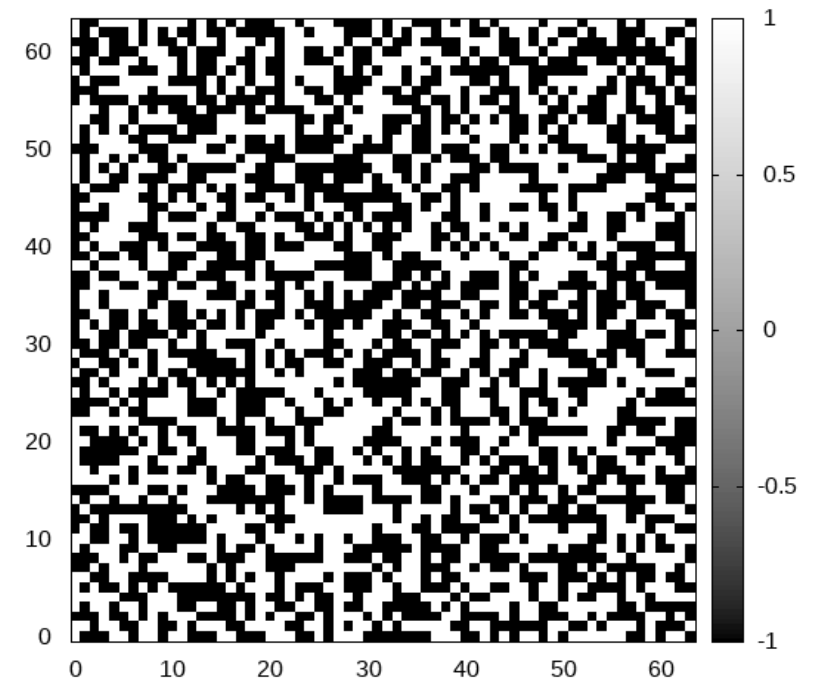
\includegraphics[width=0.425\textwidth]{Imagenes/AleatorioIsingMomento1.png}}
    \subfigure[Distribución anterior con $m \neq 0$.]{
        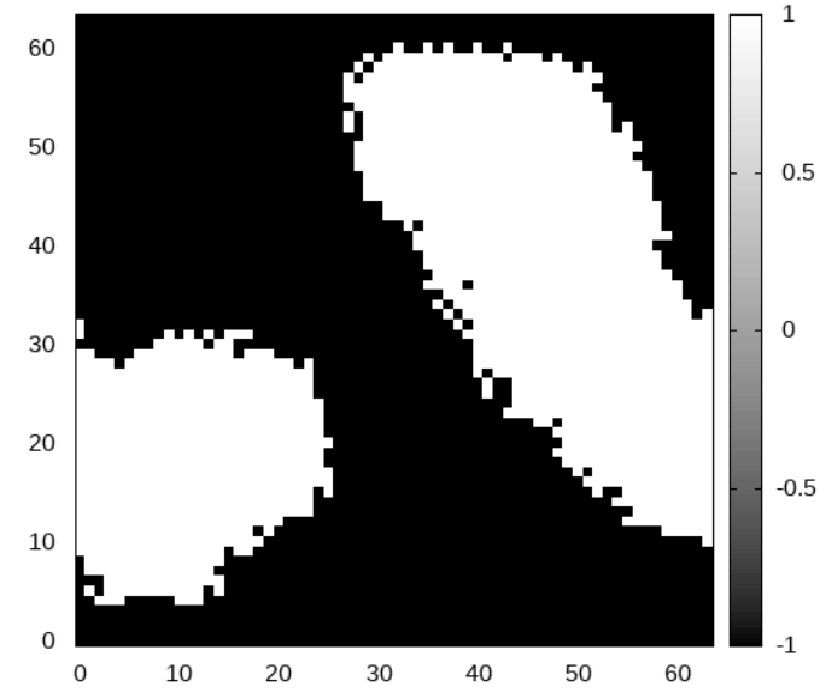
\includegraphics[width=0.425\textwidth]{Imagenes/AleatorioIsingMomento2.png}}
        
    \label{EjemploIsing}
    \\
        
    \caption{Imágenes que representan las variaciones y desarrollo en la distribución de estados $s_{ij}$ de un material tras un determinado tiempo aproximado ($\Delta t$) siguiendo el modelo de Ising-Kawasaki y una temperatura de $0.75K$, con condiciones de contorno periódicas.}
    
    \subfigure[Distribución aleatoria de $s_{ij}$ con $m=0$.]{
        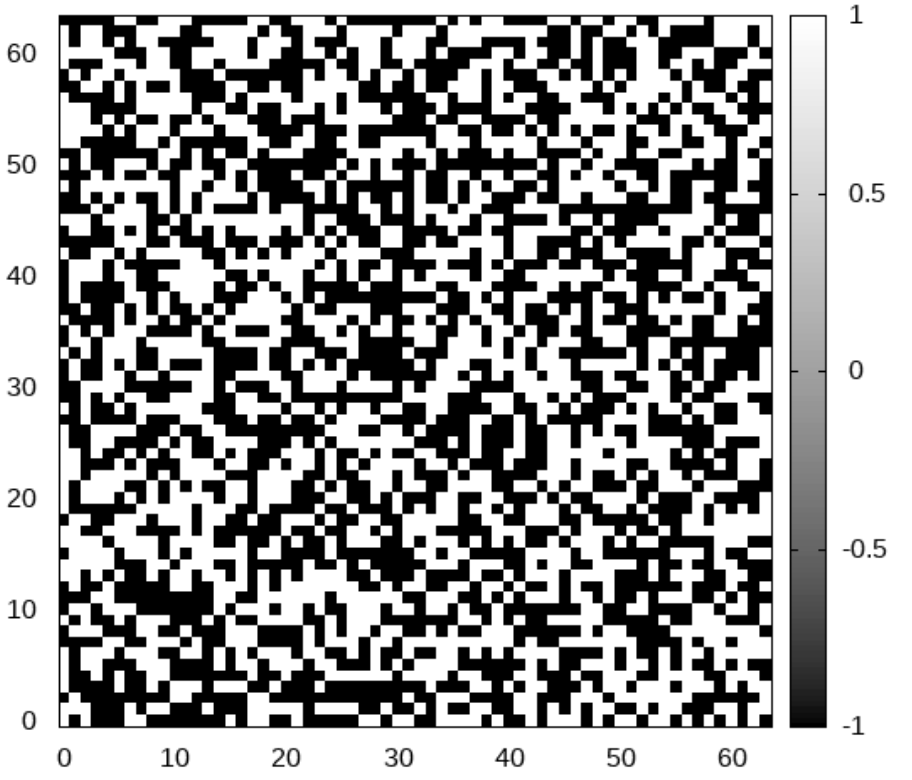
\includegraphics[width=0.425\textwidth]{Imagenes/AleatorioIsingKawasakiMomento1.png}}
    \subfigure[Distribución anterior con $m = 0$.]{
        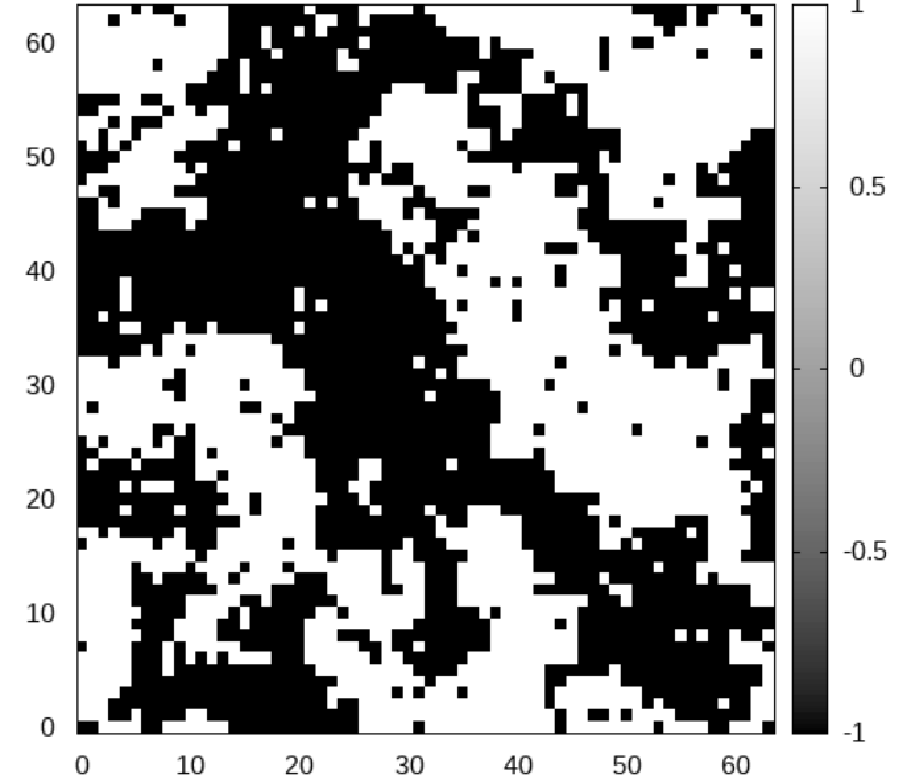
\includegraphics[width=0.425\textwidth]{Imagenes/AleatorioIsingKawasakiMomento2.png}}

    \subfigure[Distribución $s_{ij}$ tras un tiempo $\Delta t$ bastante mayor a los anteriores y para $T=0.65K$.]{
        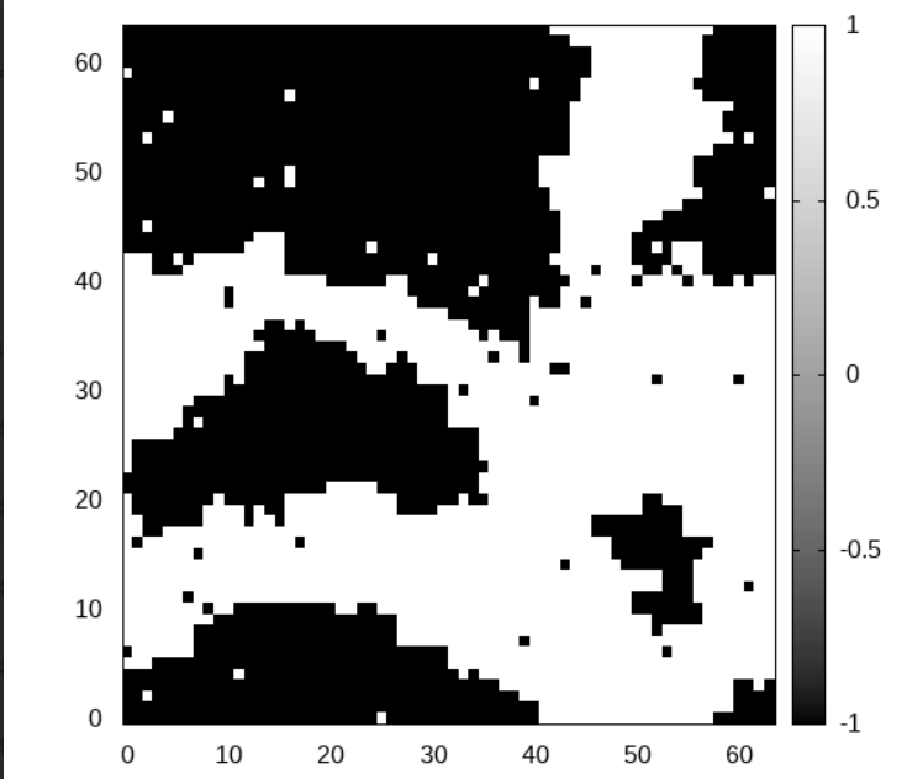
\includegraphics[width=0.425\textwidth]{Imagenes/IKDistparabajaTejemplocomp.png}}
    
    \label{EjemploIsingKawasaki}
    
  \end{center}
\end{figure}\\

\newpage

\begin{figure}[H]
    
  \begin{center}

    \caption{Imágenes que representan las variaciones y desarrollo en la distribución de estados $s_{ij}$ de un material tras un determinado tiempo aproximado ($\Delta t$) siguiendo el modelo de Ising-Kawasaki para diferentes temperaturas, con condiciones de contorno fijas en el eje $y$ y periódicas en el $x$. Y una distribución fraccionaria inicial de $x = 0.5 \rightarrow m = 0$.}
    \label{fig3}
    \subfigure[Distribución inicial $s_{ij}$ para $m=0$.]{
        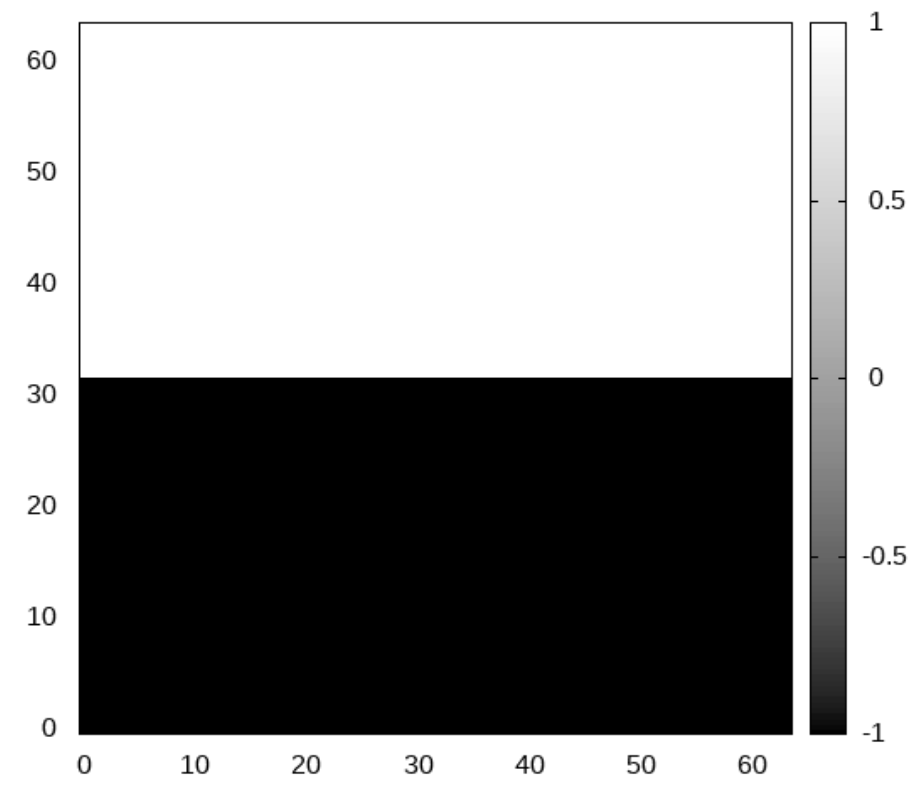
\includegraphics[width=0.45\textwidth]{Imagenes/IsingKawasakiX50.png}}
    \subfigure[Distribución con $T = 0.65K$.]{
        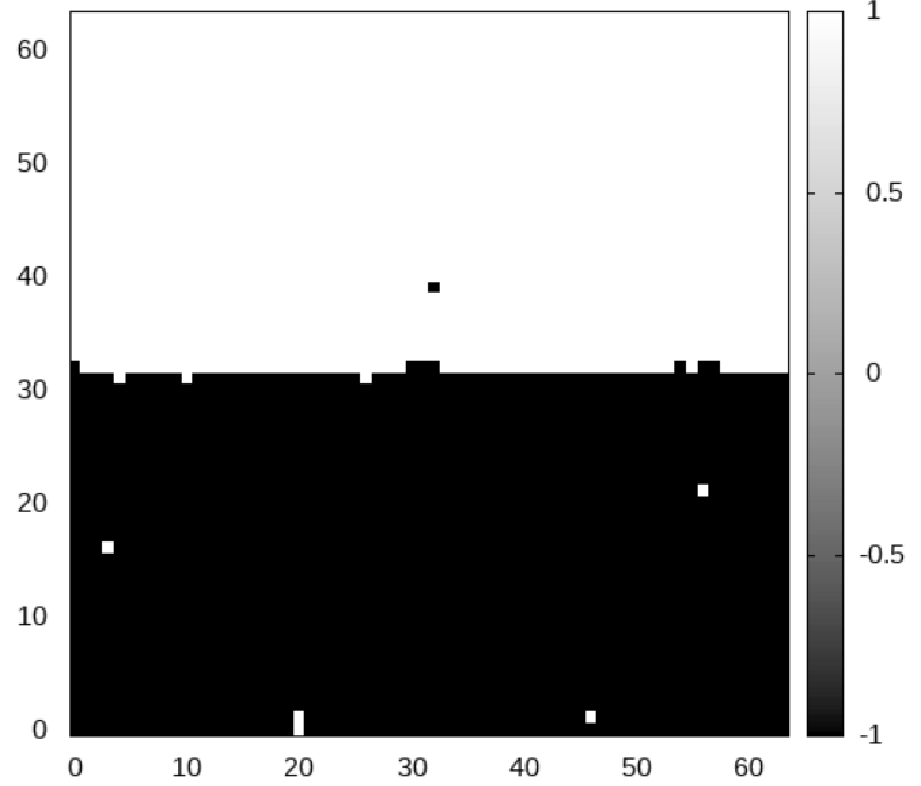
\includegraphics[width=0.45\textwidth]{Imagenes/IsingKawasakiX50T05DT.png}}
    \subfigure[Distribución con $T = 0.8K$.]{
        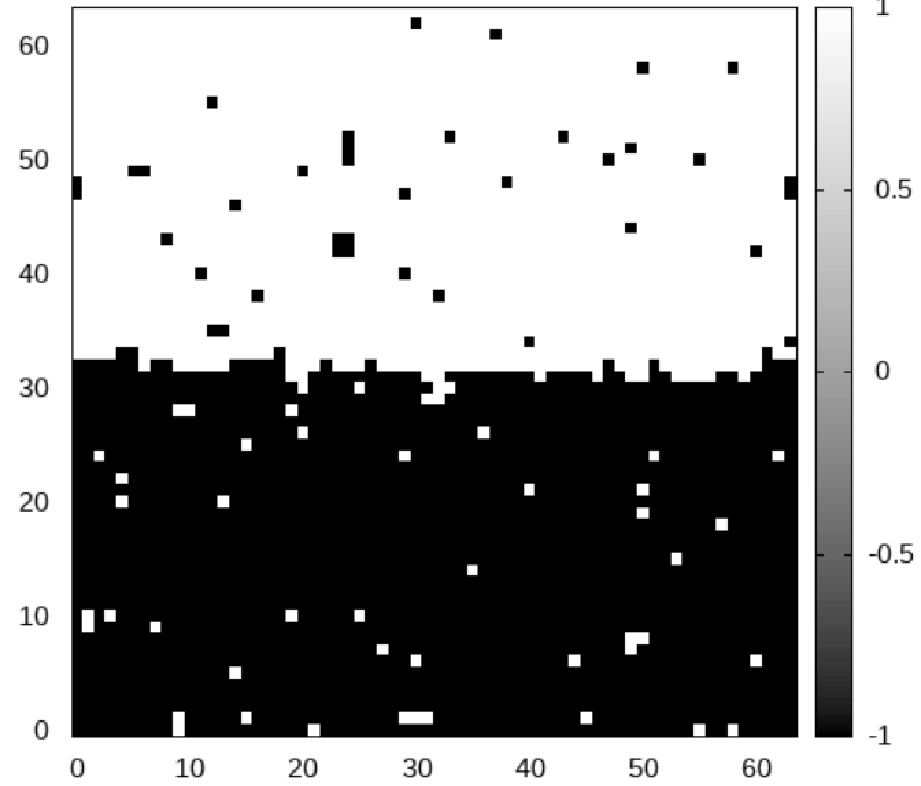
\includegraphics[width=0.45\textwidth]{Imagenes/IsingKawasakiX50T075DT.png}}
    \subfigure[Distribución con $T = 0.85K$.]{
        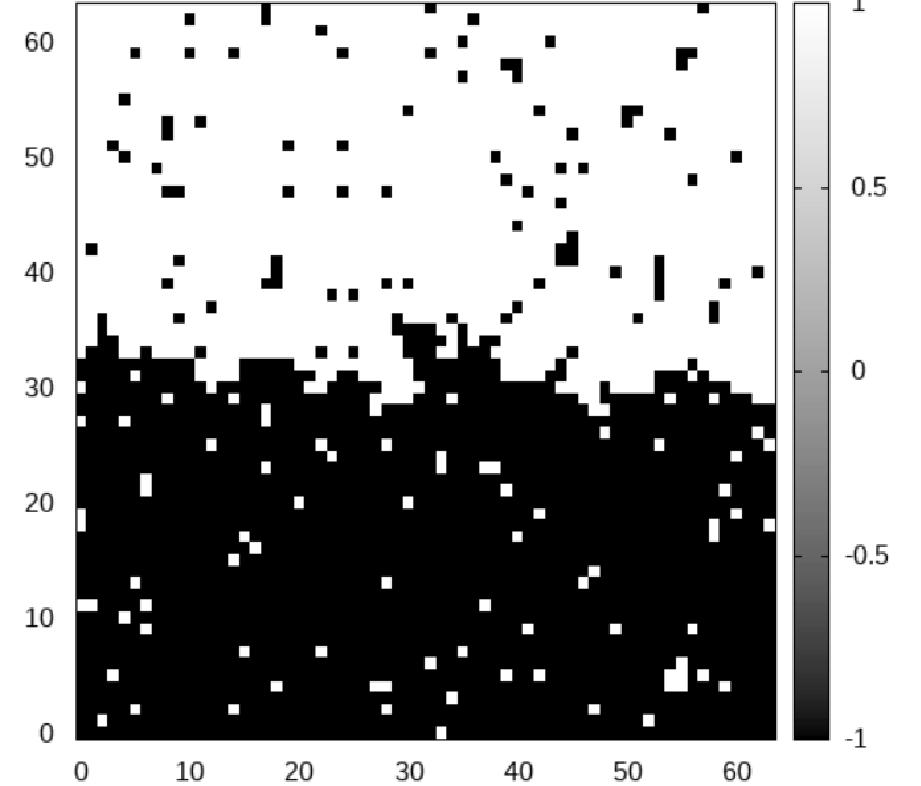
\includegraphics[width=0.45\textwidth]{Imagenes/IsingKawasakiX50T08DT.png}}  
    \subfigure[Distribución con $T = 5K$.]{
        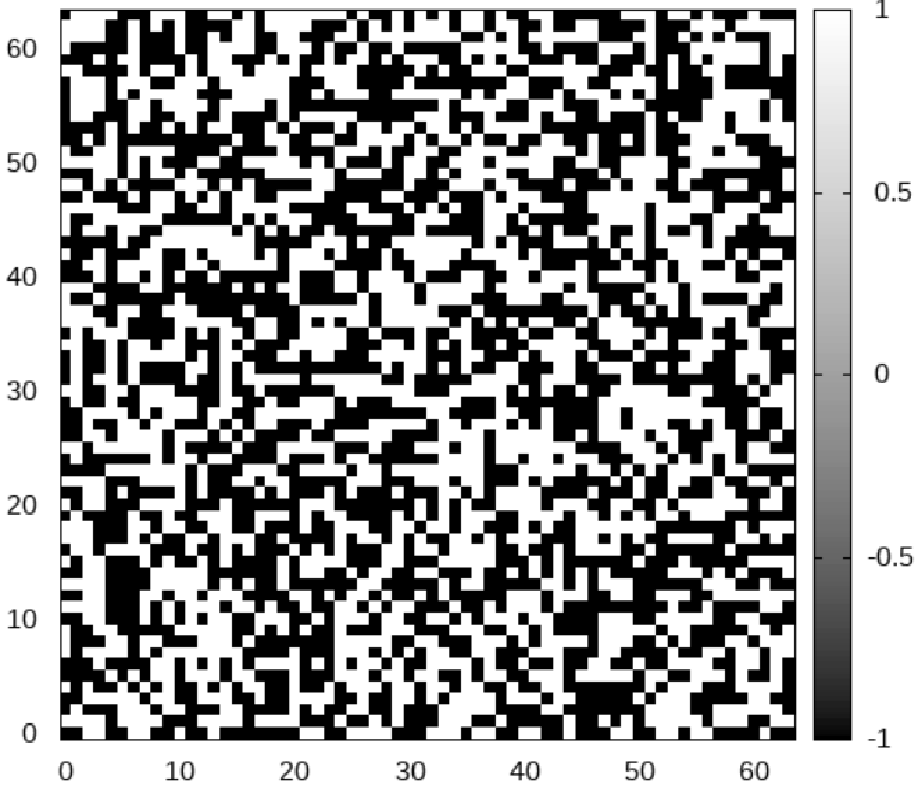
\includegraphics[width=0.45\textwidth]{Imagenes/IsingKawasakiX50T5.png}}      
  \end{center}
\end{figure}\\

\newpage

\begin{figure}[H]
 
  \begin{center}        
    \caption{Imágenes que representan las variaciones y desarrollo en la distribución de estados $s_{ij}$ de un material tras un determinado tiempo aproximado ($\Delta t$) siguiendo el modelo de Ising-Kawasaki para diferentes temperaturas, con condiciones de contorno fijas en el eje $y$ y periódicas en el $x$. Y una distribución fraccionaria inicial de $x = 0.9 \rightarrow m = 0.8$.}
    \label{fig4}
    \subfigure[Distribución inicial de $s_{ij}$ con $m=0.8$.]{
        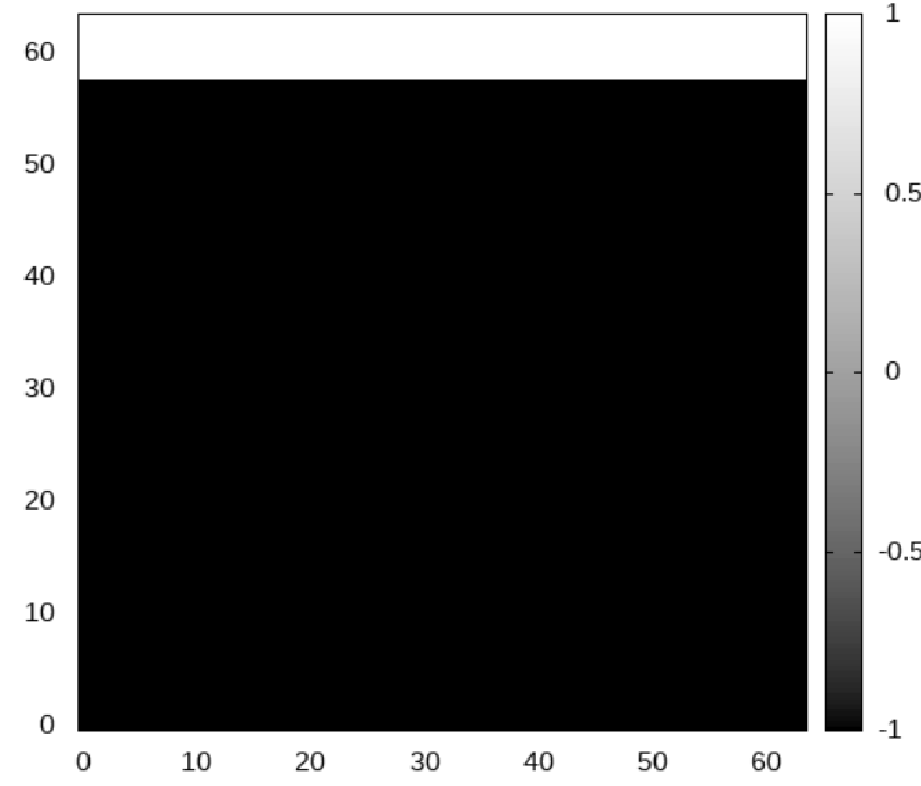
\includegraphics[width=0.45\textwidth]{Imagenes/IsingKawasakiX90.png}}
    \subfigure[Distribución con $T = 0.65K$.]{
        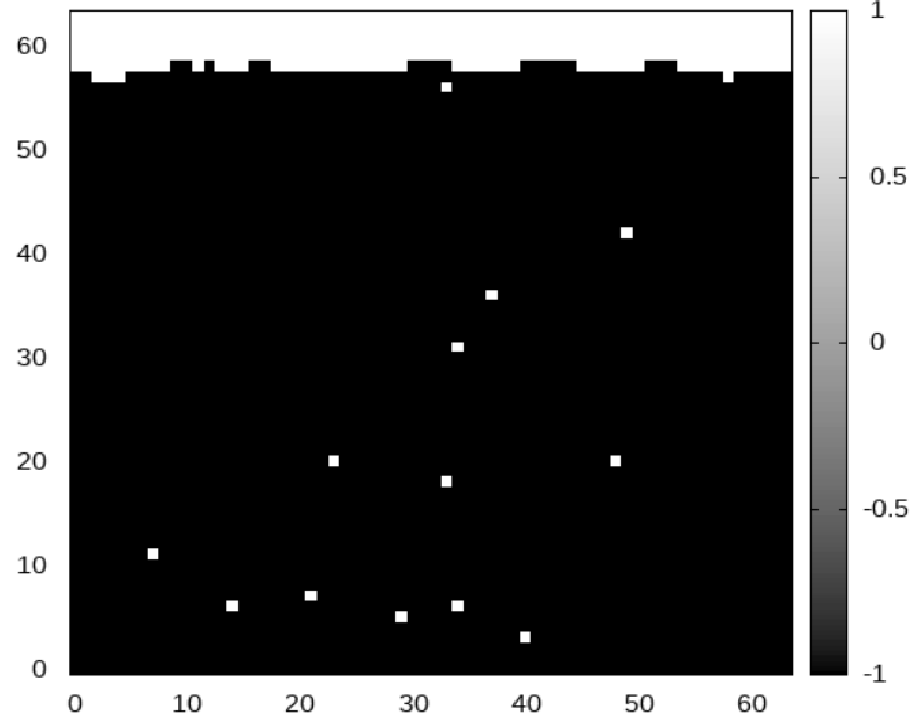
\includegraphics[width=0.475\textwidth]{Imagenes/IsingKawasakiX90T05DT.png}}
    \subfigure[Distribución con $T = 0.8K$.]{
        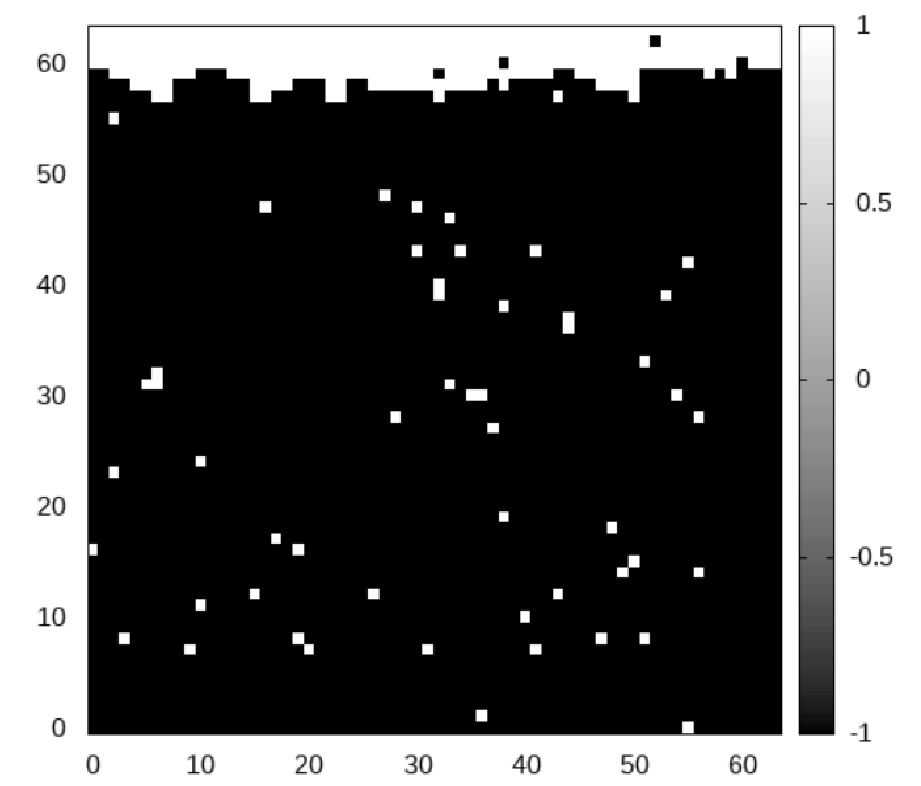
\includegraphics[width=0.45\textwidth]{Imagenes/IsingKawasakiX90T075DT.png}}
    \subfigure[Distribución con $T = 0.85K$.]{
        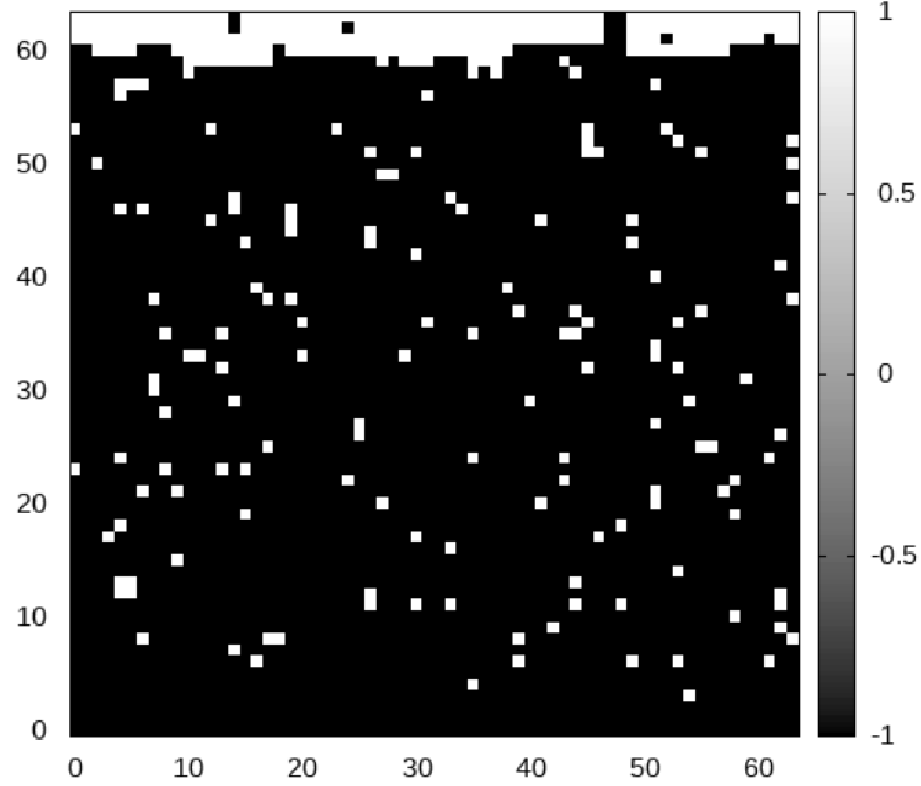
\includegraphics[width=0.45\textwidth]{Imagenes/IsingKawasakiX90T08DT.png}}  
    \subfigure[Distribución con $T = 5K$.]{
        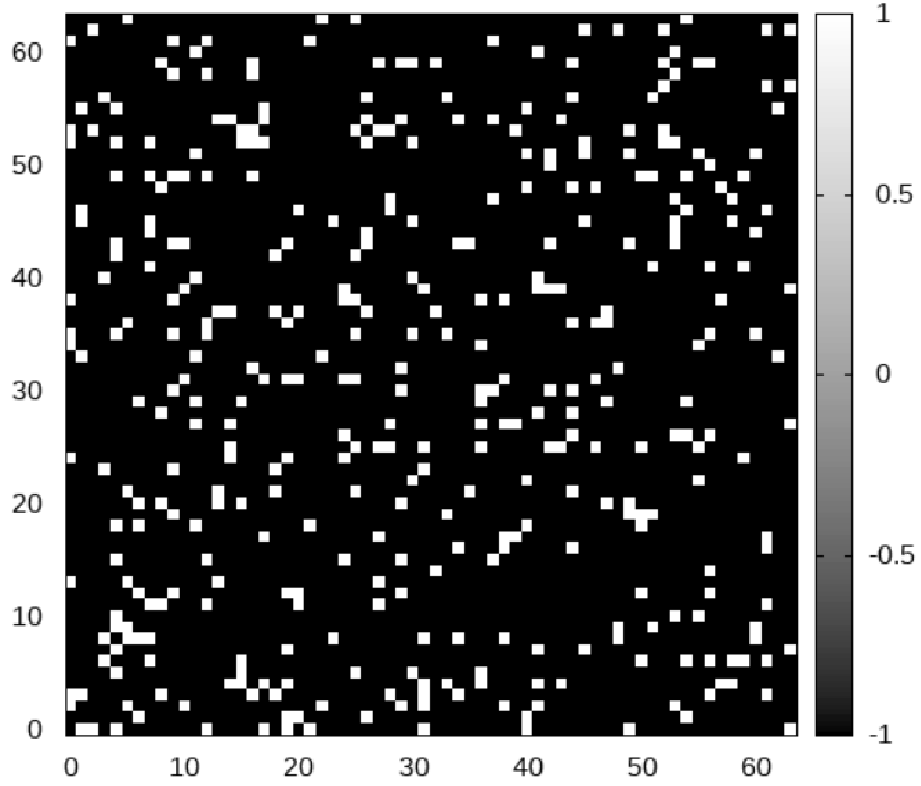
\includegraphics[width=0.45\textwidth]{Imagenes/IsingKawasakiX90T5.png}} 
    
  \end{center}
\end{figure}\\

\subsubsection{Variaciones de $C_N$ y $\chi_N$.}
Primero vamos a ver cómo varían ambas variables para diferentes temperaturas ($T$) y número de partículas ($N$).\\

El objetivo es entender que ocurre para diferentes valores de estás variables en los sistemas descritos, también visualizar con mayor claridad el resto de resultados, en los siguientes apartados, y además, tratar de encontrar la temperatura en torno a la cuál el sistema comienza a tener variaciones considerables ($T_C$). Al estudiar el comportamiento de las mismas con respecto a N, y extrapolando para el valor límite $N \rightarrow \infty$ podemos conocer $T_C$ tanto a través de $C_n$ cómo de $\chi_N$.\\

Para obtener las siguientes gráficas se han calculado dichas variables para 50 temperaturas $T = 0.1 \hspace{1mm} K, \hspace{1mm} 0.2 \hspace{1mm} K, \hspace{1mm} ..., \hspace{1mm} 5 \hspace{1mm}K$, y para $N = 32, \hspace{1mm} 64 \hspace{1mm} y \hspace{1mm} 132 \hspace{1mm}$ partículas.\\

Si tenemos en cuenta la expresión \ref{eq5} y despejamos la ecuación \ref{eq7} obtenemos una expresión tal que $\chi(M,N,T) = \alpha(M,N)/T$, siendo $\alpha(N,T)$ una constante que se mantiene para todo M y T, que ha sido teóricamente calculado para cada uno de los casos, y quedando $\chi$ aproximadamente cómo una función del tipo $y(x) = cte/x$.\\
\begin{equation}
    (\chi_N)_{Teorico} = [\frac{M^2}{N^3} (1- \frac{1}{N})] \frac{1}{T} = \alpha(M,N) \frac{1}{T}
\end{equation}

Cabe recalcar que $\alpha \propto 1/N^3$, lo cuál explica que para mayores N, $T_C$ se acerque mucho más a 0 que en el resto de los casos.\\

El caso de $C_N$ es más complejo, pues la energía no se mantiene constante con respecto a las temperaturas, pero comparando ambas gráficas podemos hacernos a la idea de donde encontramos las temperaturas relevantes y en los que estudiar el modelo con más ainco. Aun así cabe destacar que $C_N \propto \frac{1}{N^3}$ también, por lo que denotaremos claramente cómo para mayores N, la curva más se acercará 0, y por otro lado está claro que $C_N$ se asemejará a una función del tipo $y(x) = cte/x^2$, ya que $C_N \propto \frac{1}{T^2}$. Lo denotamos claramente en las siguientes gráficas donde se han realizado ajuste a dicha funciones tipos para denotar dichas variaciones y semejanza al modelo teórico.\\

Puntualizar, que aunque no tenga sentido físico, para el caso de los valores $\chi$ por dominios, en la partición $x=0.5$, se ha considerado que para el dominio de estado inicial -1, $\chi$ es negativo, y por contrapartida, para +1, es positivo. Viendo la gráfica podemos entenderlo mejor y más visualmente, de forma que la variación de la $\chi_N$ total del sistema es el resultado de la suma de ambas variaciones por dominios de manera aproximada, es decir, realmente la suma de $\chi_N$ por dominios no son aditivos y no dan exactamente el valor real. Esto no se ha tenido en cuenta para el caso de $x=0.9$\\


Debido al gran tamaño de las imágenes, la gran cantidad de datos y a las limitaciones del documento es imposible ver las imágenes con denótale claridad, por esta misma razón haciendo clic en el siguiente enlace se pueden ver todas las imágenes de este trabajo con mucha mayor claridad: {\underline{\href{https://drive.google.com/drive/folders/1ivzNfi-jLKLyxUTFhOSw3gwLT2m2QSXb?usp=sharing}{gráficas con mucha mayor resolución}}}.

\begin{figure}[H]

  \begin{center}  
  
  
    \caption{Variaciones de $\chi_N$ para $m=0$ o $x = 0.5$.}
    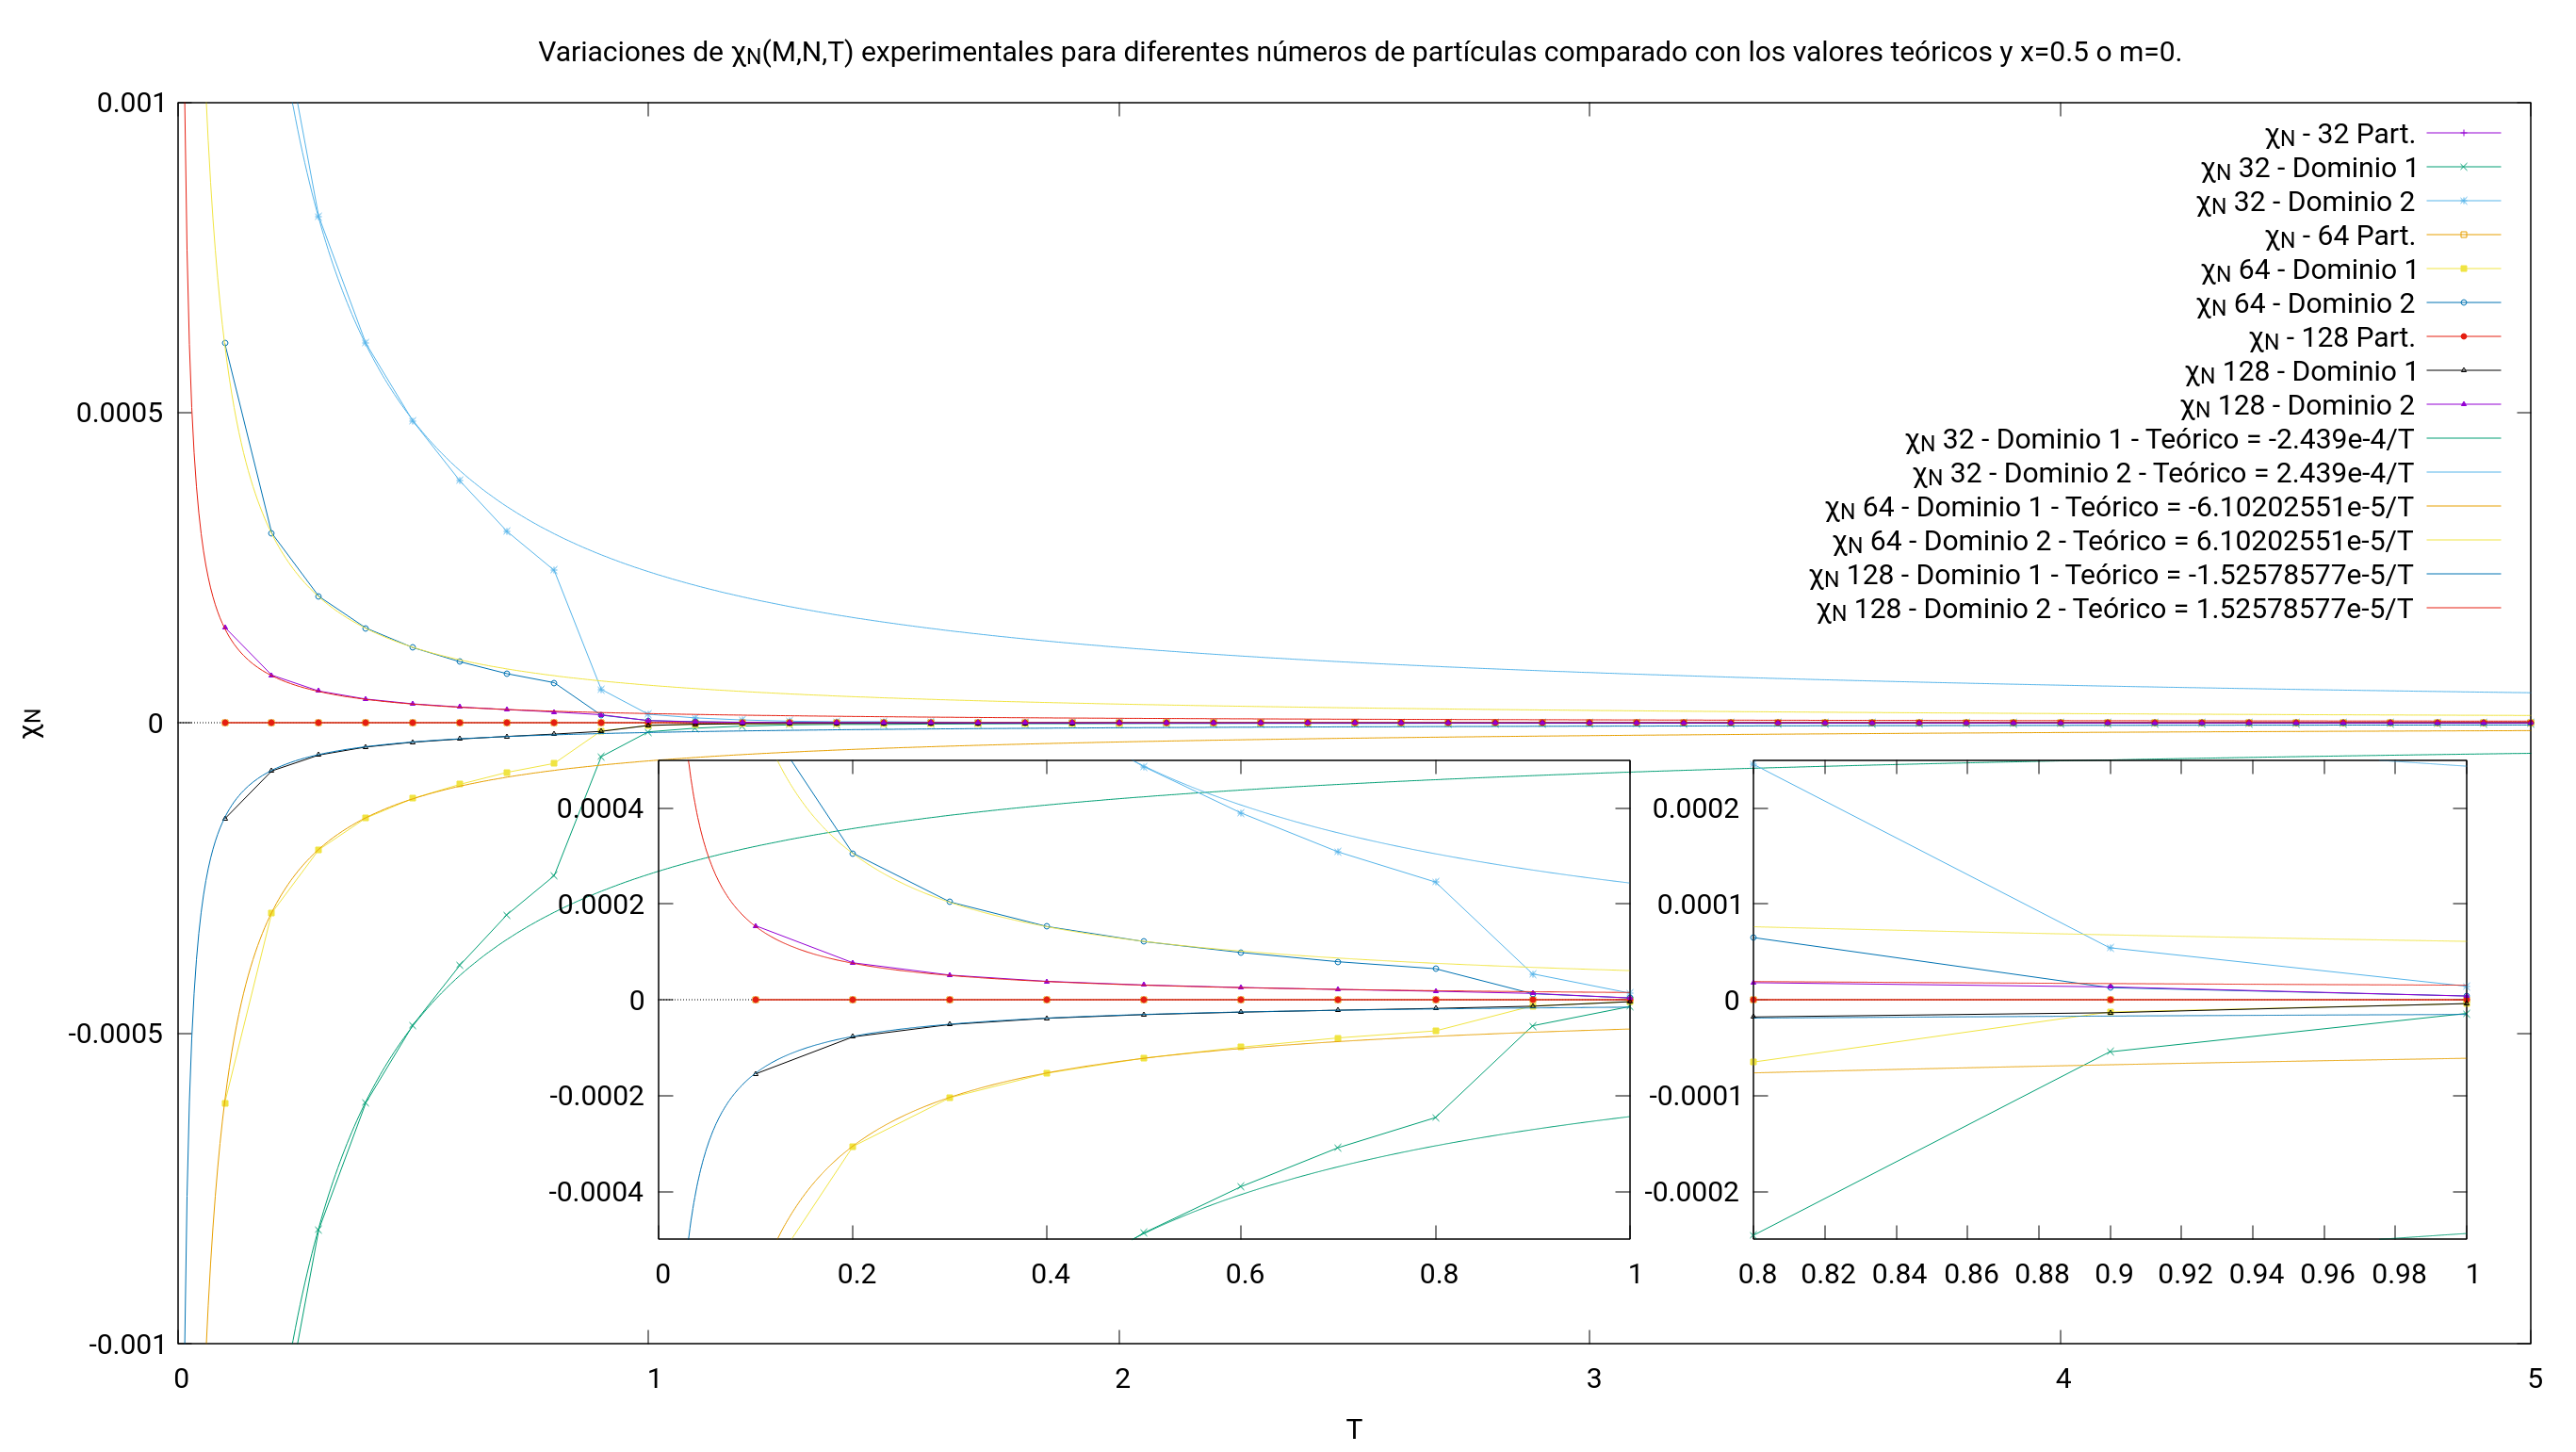
\includegraphics[width=1.1\textwidth]{Imagenes/XN(T)-P50.png}}  
    \label{xn05}
  \end{center}
\end{figure}\\

\begin{figure}[H]

  \begin{center}  
  
  
    \caption{Variaciones de $C_N$ para $m=0$ o $x = 0.5$.}
    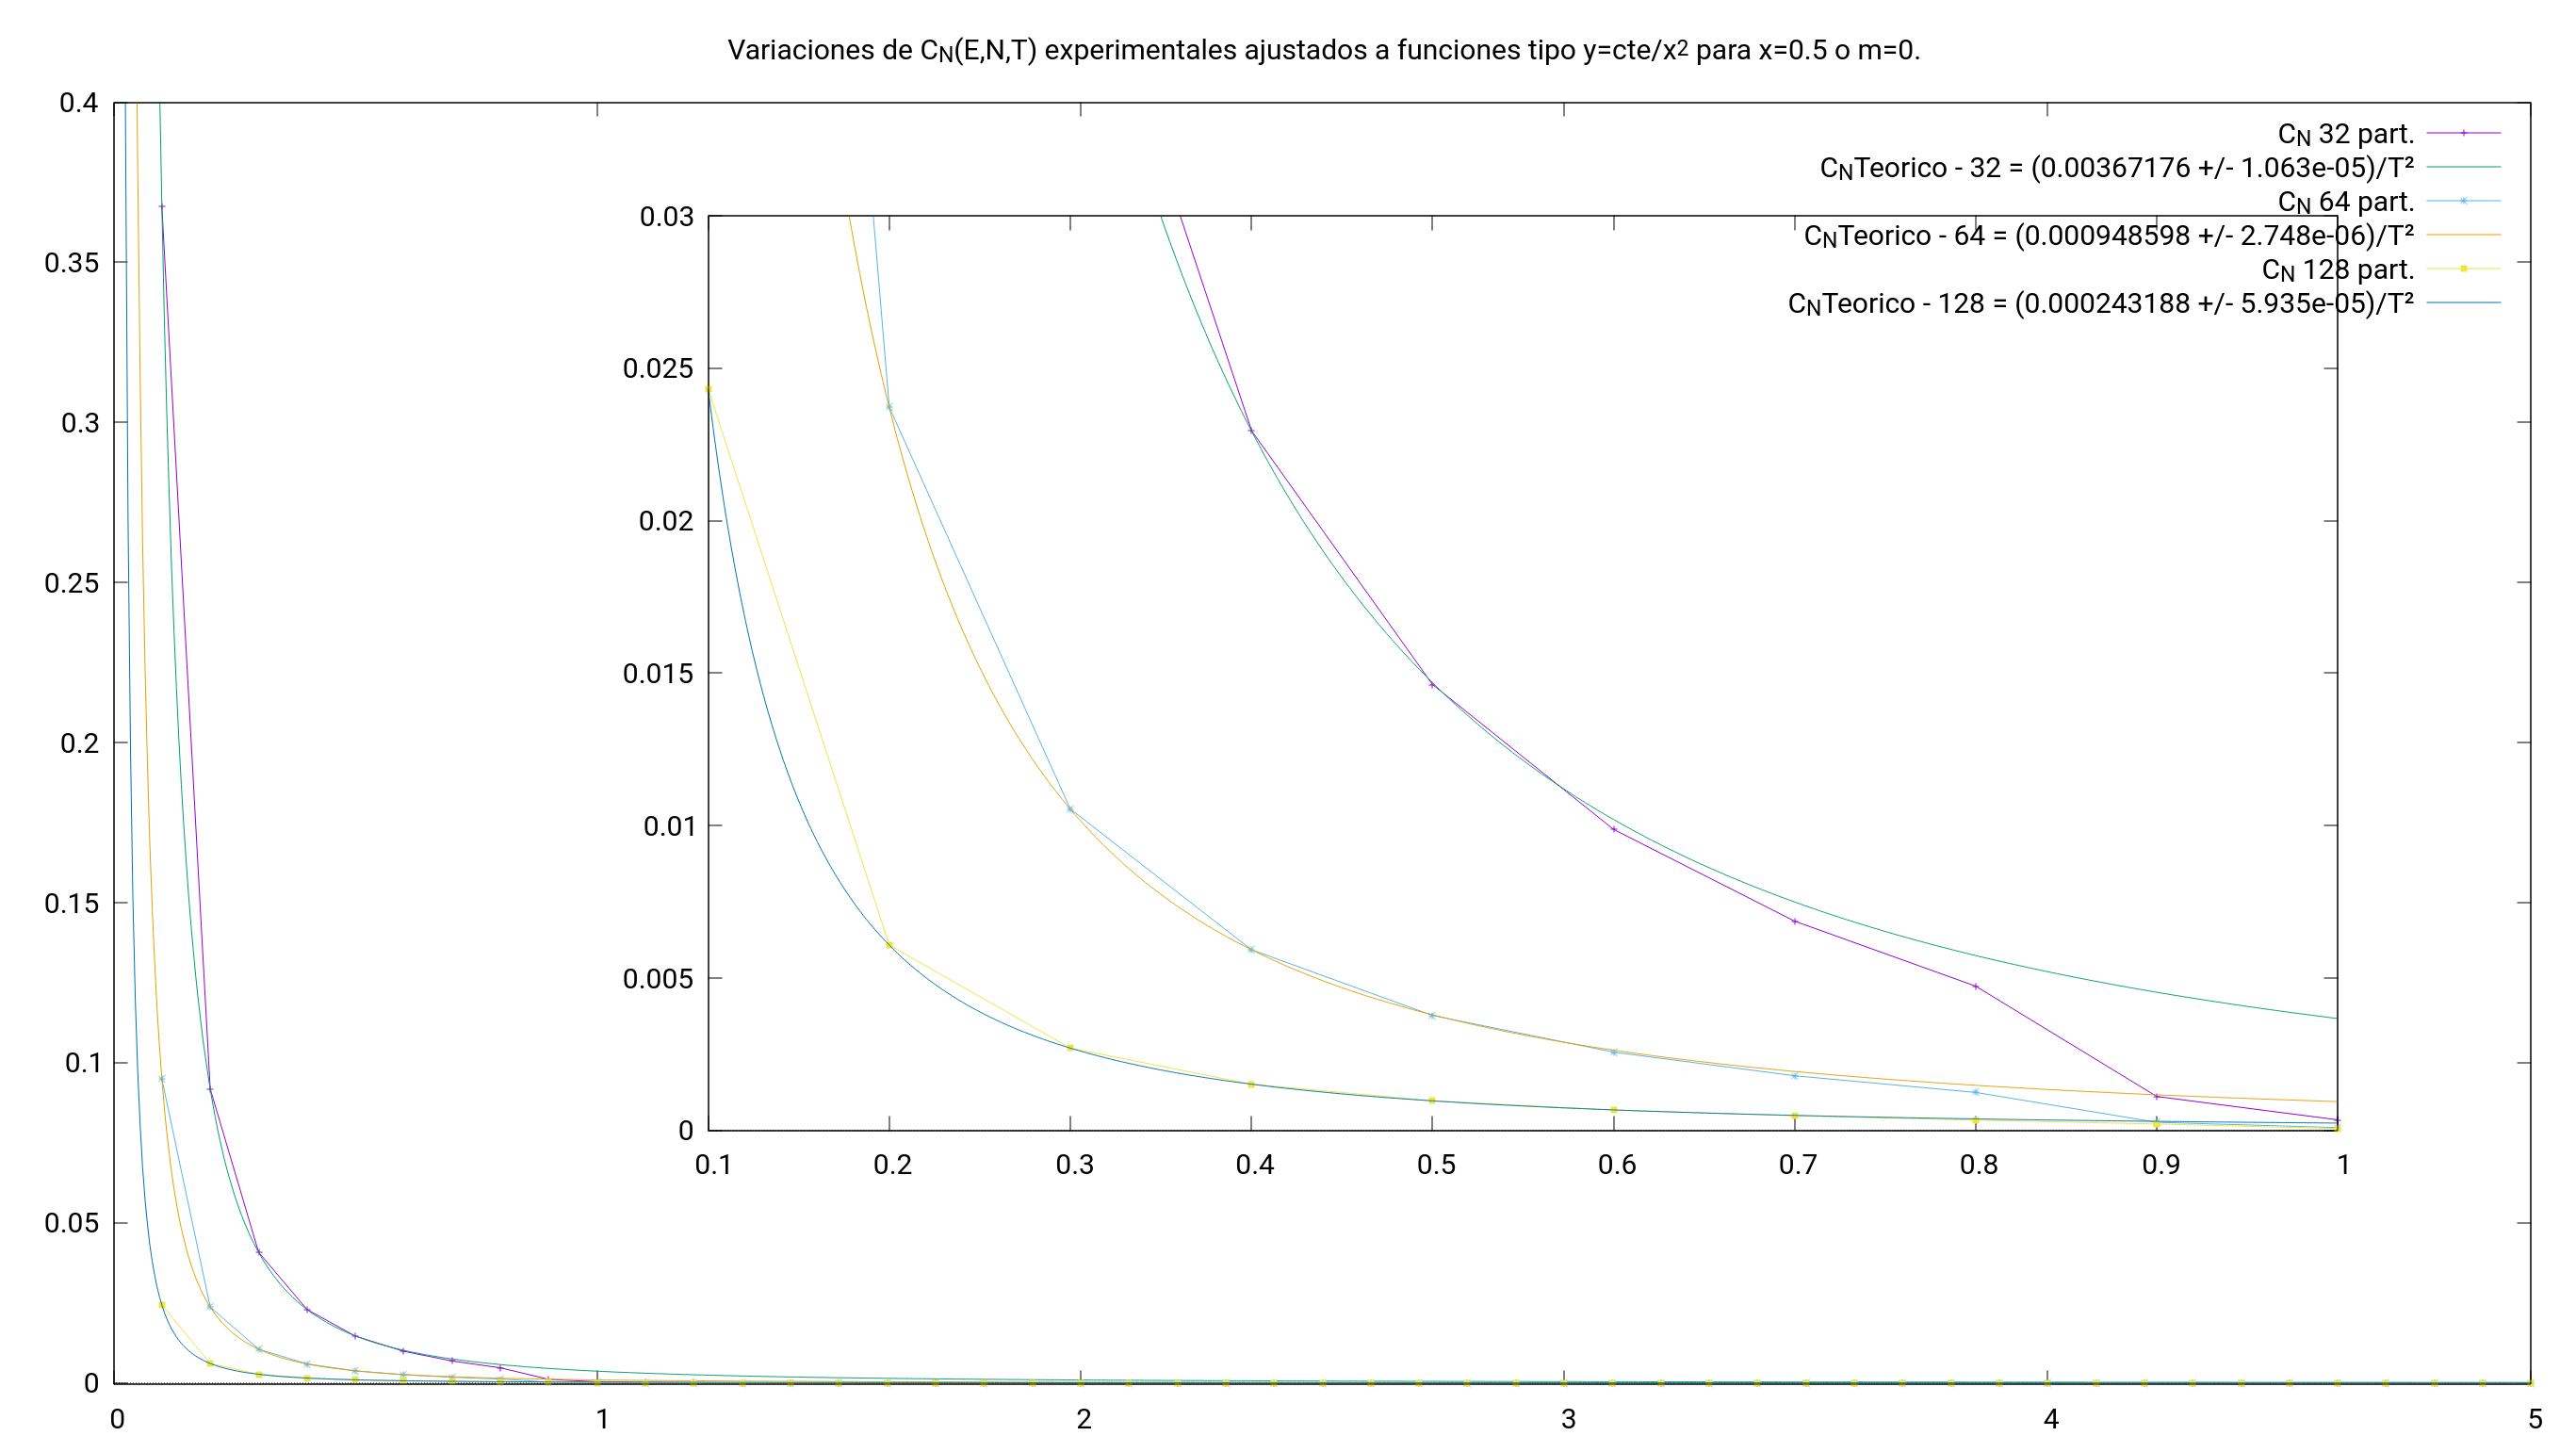
\includegraphics[width=1.1\textwidth]{Imagenes/CN(T)-P50.png}}    
    \label{cn05}
  \end{center}
\end{figure}\\

\begin{figure}[H]

  \begin{center}      
  
    \caption{Variaciones de $\chi_N$ para $m=0.8$ o $x = 0.9$.}
    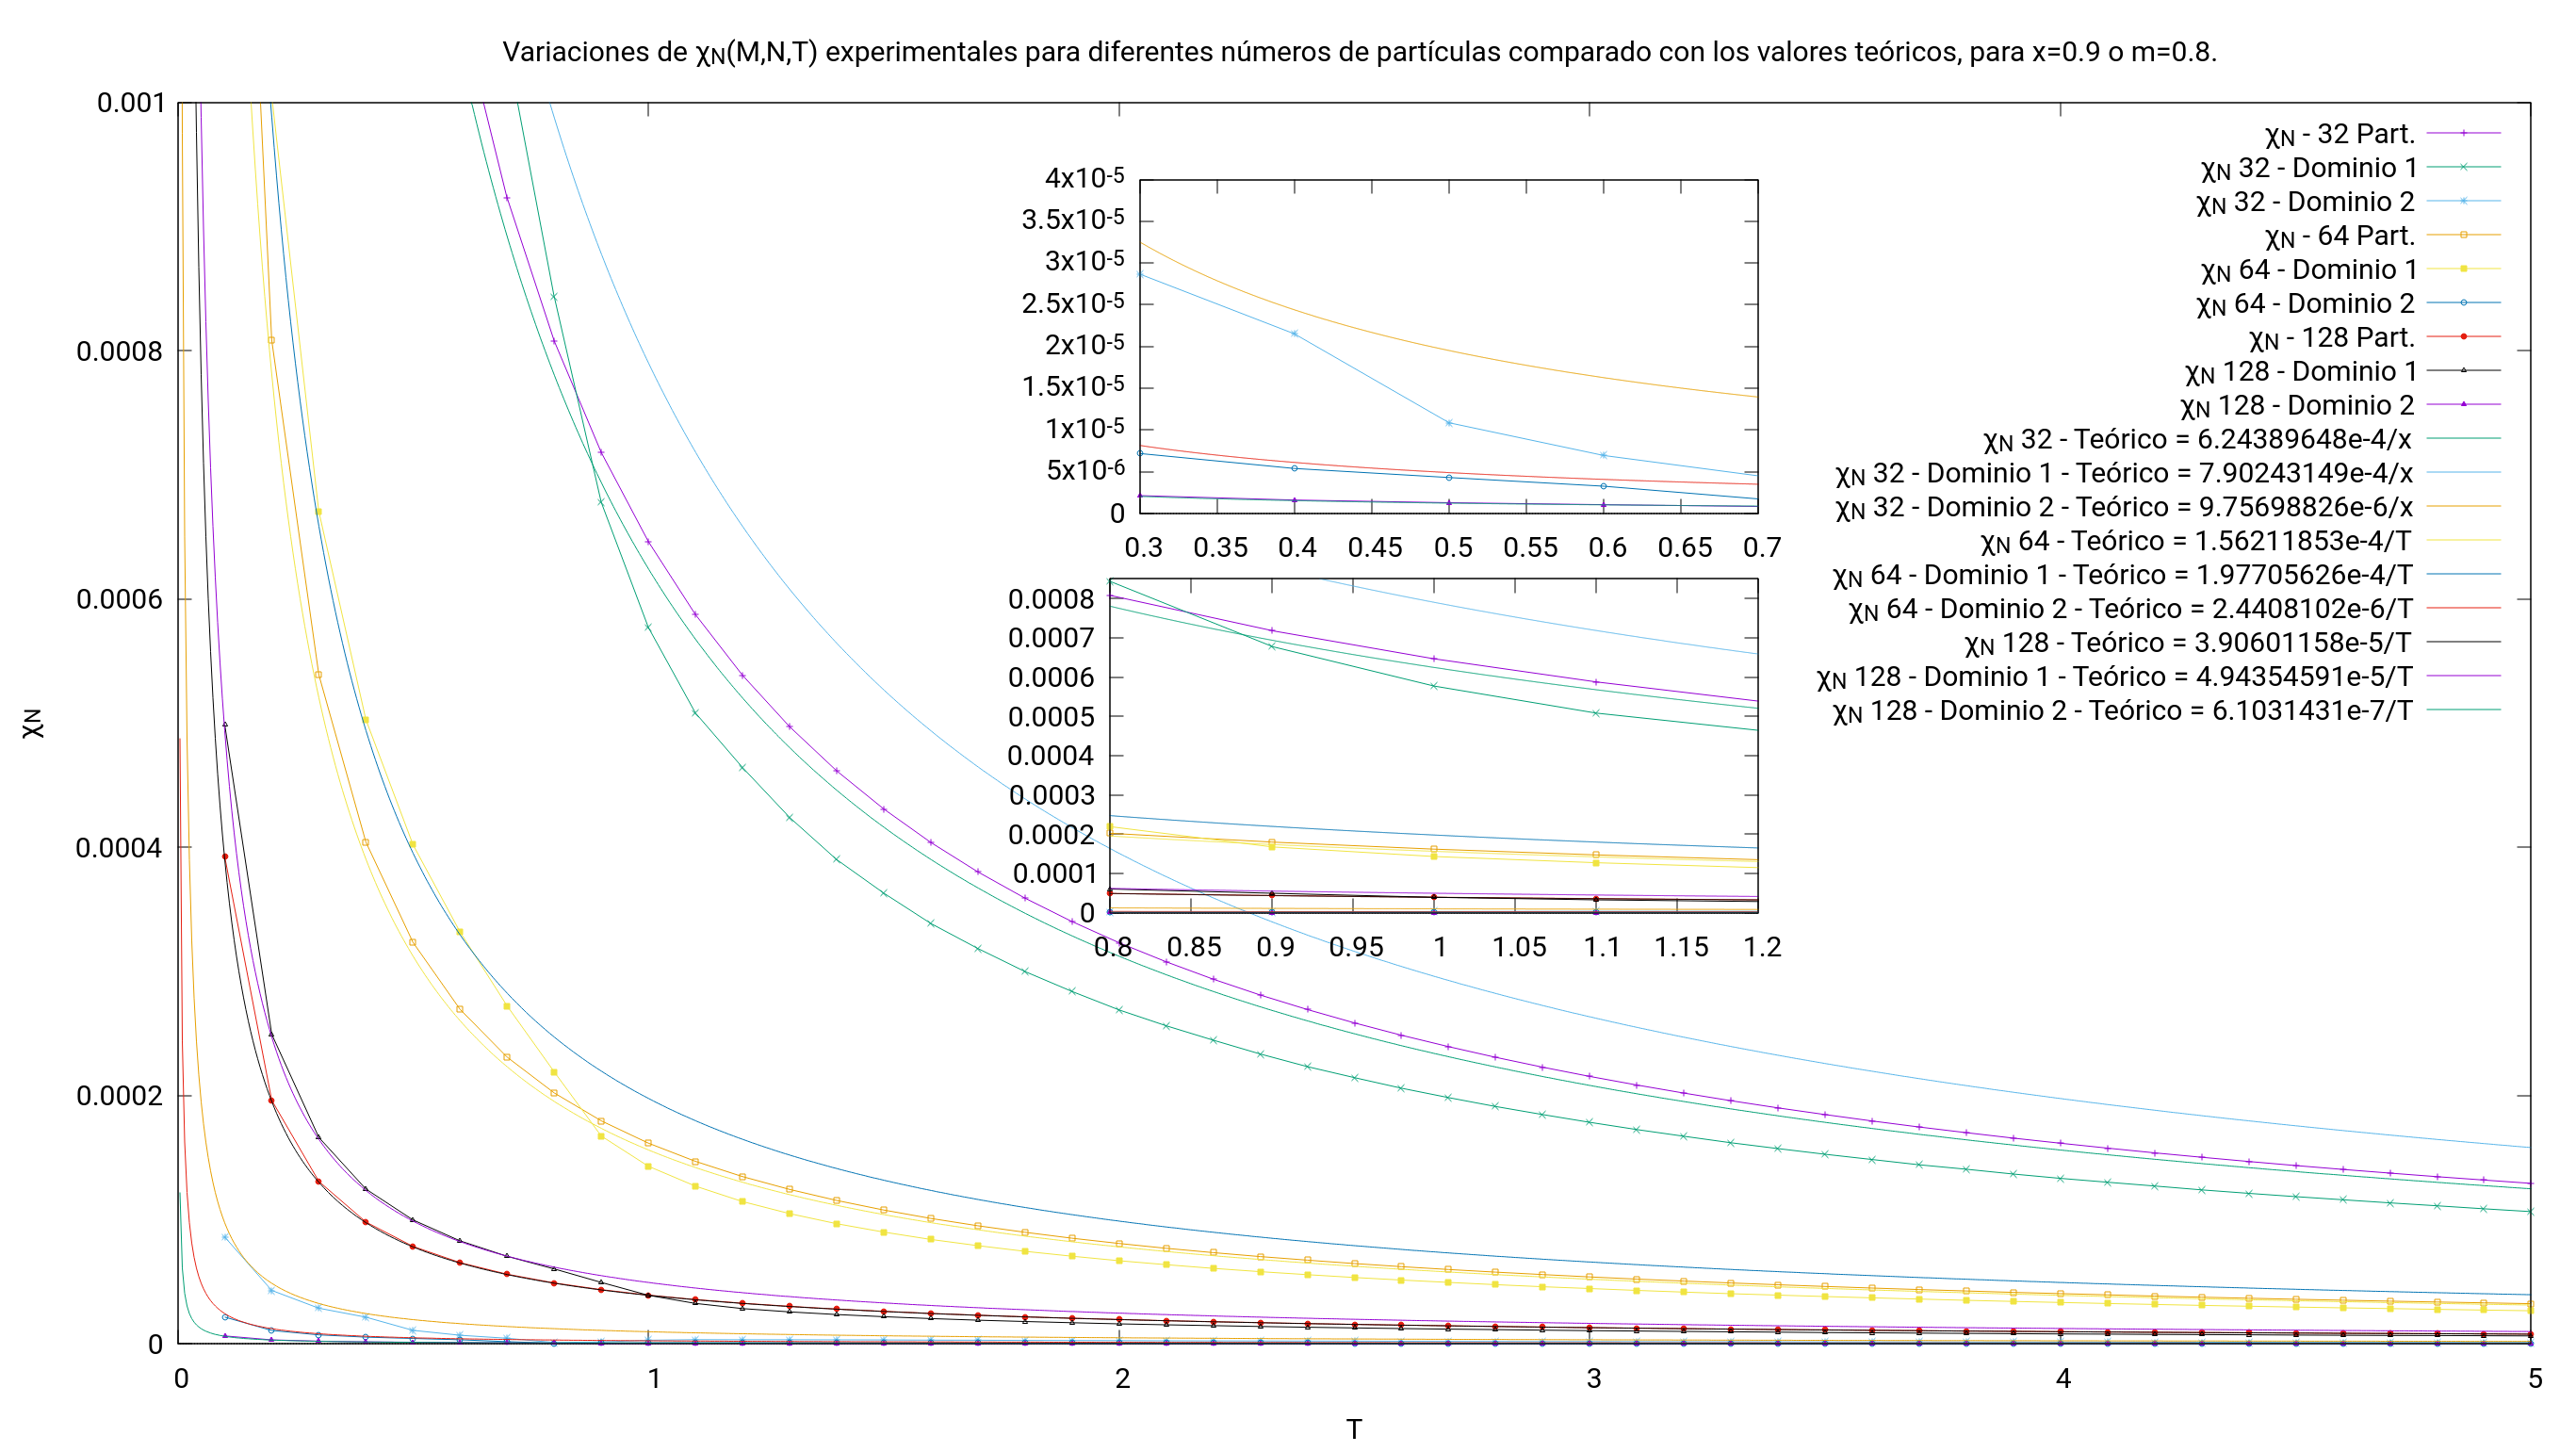
\includegraphics[width=1.1\textwidth]{Imagenes/XN(T)-P90.png}} 
    \label{xn09}
  \end{center}
\end{figure}\\

\begin{figure}[H]
\begin{center}   

   
    \caption{Variaciones de $C_N$ para $m=0.8$ o $x = 0.9$.}
    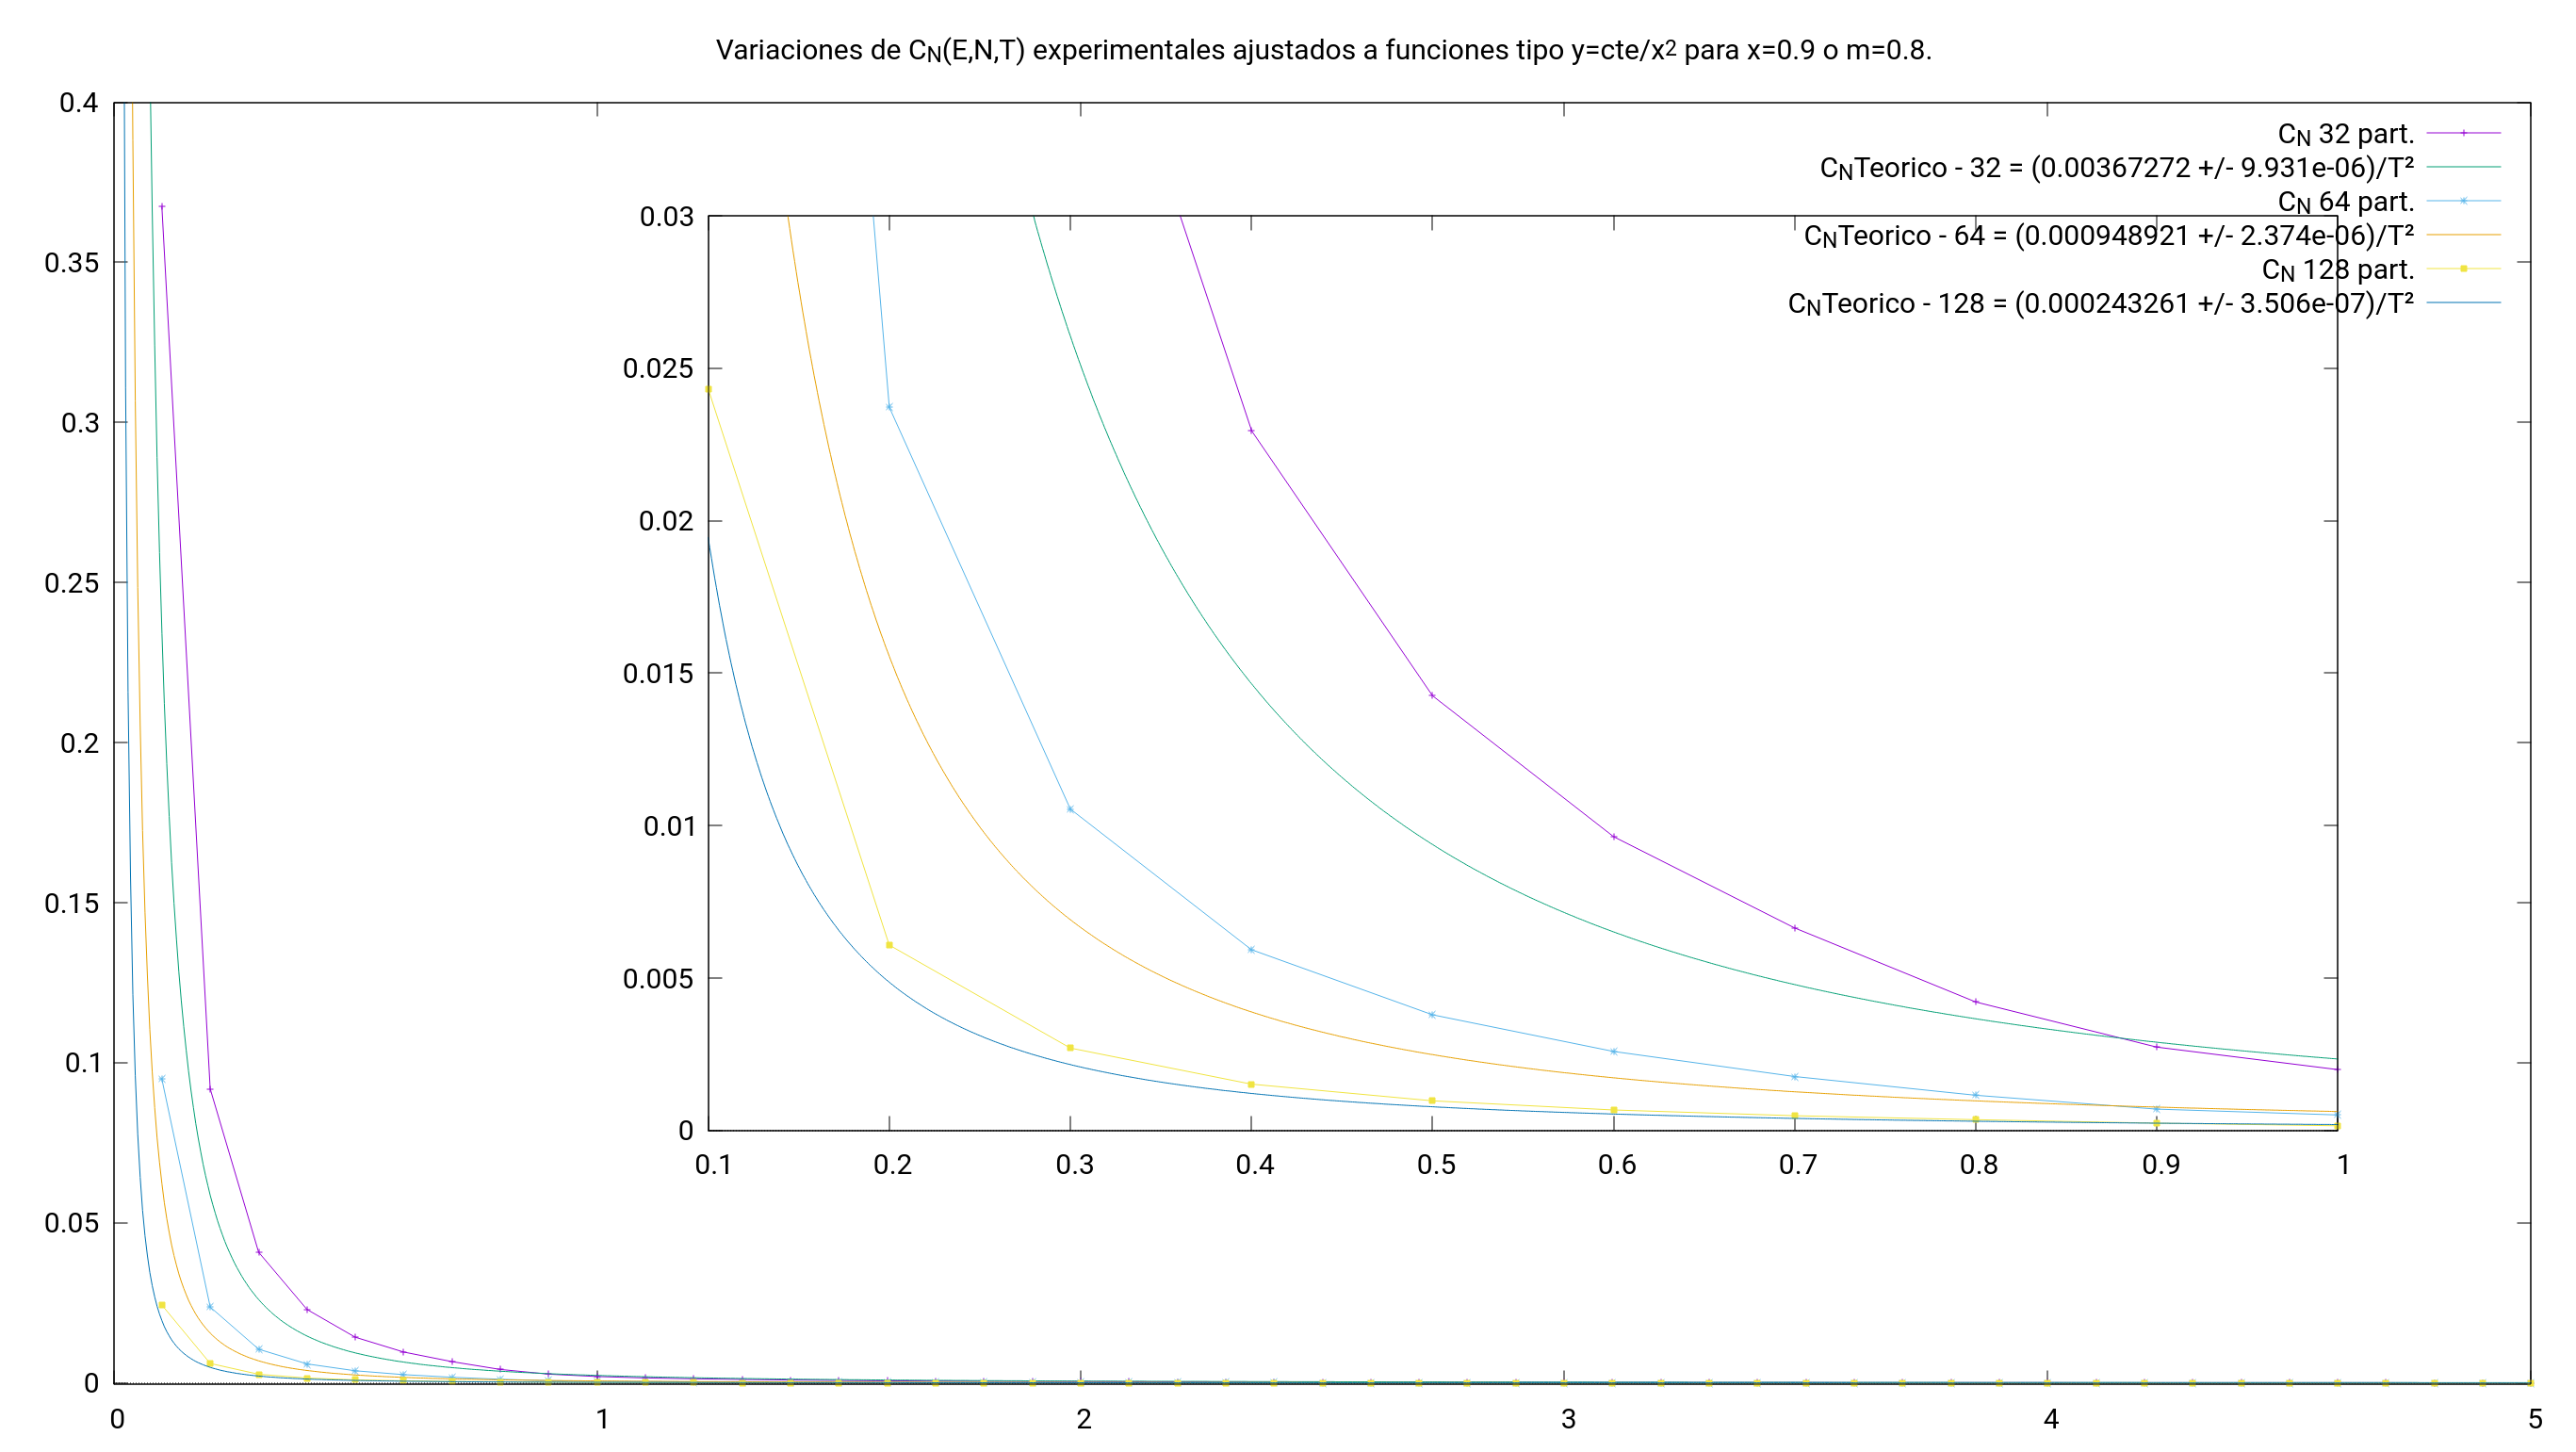
\includegraphics[width=1.1\textwidth]{Imagenes/CN(T)-P90.png}} 
    \label{cn09}
  \end{center}
\end{figure}\\

Claramente vemos que los resultados se ajustan generalmente bastante bien a los modelos considerados.\\

Cabe denotar que ambos valores se hacen máximos cuando $T \rightarrow 0$, por lógica en dicho punto encontraremos que la energía del sistema es máxima y que las variaciones de la magnetización por dominios son completamente nulas pues el sistema es completamente estable y mantiene su estado de magnetización.\\

Si extrapolamos las variancias de ambas variables con respecto a $N$, cuando $N \rightarrow \infty$, denotamos 2 puntos de gran relevancia. Primero que cuanto más nos acercamos a 1 mayor es la tendencia a hacerse los valores 0, siendo un punto de vital importancia el de $T=0.9K$ e incluso alejándose de los valores supuesto teóricos sobretodo para casos de menor número de partículas. Y segundo, a partir del intervalo $T \in [0.4,0.6]K$ hacia menores temperaturas la curva crece extremadamente rápido en comparación al resto de puntos.\\

Si estudiamos que es lo que ocurre para las distribuciones $s_{ij}$ en esos puntos detonamos que por debajo de $T=0.5K$ las variaciones de la misma se hacen mínimas o nulas, y conforme nos vamos acercando a $T=0.9K$ comienzan a aumentar y a formarse dominios magnéticos de diferentes formas, quedando a partir de $T=0.91K$ un estado parecido al \ref{EjemploIsingKawasaki}.c.\\
Para 20000 pasos Montecarlo, y tras estudiar el entorno en $T=0.9K$, la distribución se mantiene relativamente estable para casi todo los puntos de los mismos, por lo que vamos a suponer que $T_C = 0.9K$. Seguramente, al comprobar para mayores lapsos de tiempo podríamos denotar que tal vez $T_C$ no es el supuesto, pero dado que en este caso necesitamos una gran cantidad de pasos Montecarlo para descubrirlo, y el dispositivo utilizado no es capaz de calcular para mayor cantidad de los mismos, vamos a suponer que es el propuesto. En cualquier caso debe ser un punto cercano y por debajo de $0.9K$.\\

Para terminar y para entender la importancia de este modelo, un material es magnetizable o paramagnético cuando $\chi>0$, es decir, con este modelo podemos visualizar como a priori el material tratado generalmente es magnetizables para casi todas sus temperaturas. Y, por otro lado, se sabe que un material es ferromagnético cuando $\chi \rightarrow \infty$. Recordemos que este modelo trata de explicar el ferromagnetismo de ciertos materiales cuando alcanza temperaturas cercanas a 0, lo cuál cuadra perfectamente con los resultados obtenidos y con todo lo explicado con anterioridad.\\
El calor especifico por otra parte, y termodinámicamente hablando, mide aproximadamente la pendiente entre las variaciones de energía con respecto a las variaciones de temperatura $(C \propto \frac{\Delta E}{\Delta T})$. Es decir, que si sabemos que el sistema en este caso tiene energía máxima y es prácticamente invariable para temperaturas cercanas al 0, el calor especifico debe crecer infinitamente para que para pequeñas variaciones de temperatura se den variaciones considerables de energía. Cosa que vemos adecuadamente en sus correspondientes gráficas también.\\


Haciendo referencia al capítulo 5 de Newman podemos ver cómo conforme nos acercamos a $T_C$ quedan unas distribuciones tales cómo las que podemos ver en las siguientes imágenes:
\begin{figure}[H]
  \begin{center}        
    \caption{Representaciones de las variaciones y desarrollo en la distribución de estados $s_{ij}$ de un material tras un determinado tiempo aproximado ($\Delta t$) siguiendo el modelo de Ising-Kawasaki para diferentes temperaturas con respecto a $T_C$, con condiciones de contorno fijas en el eje $y$ y periódicas en el $x$. Y una distribución fraccionaria inicial de $x = 0.5 \rightarrow m = 0$.}

    \label{fig9}
    \subfigure[Distribución inicial de $s_{ij}$ con $m=0$.]{
        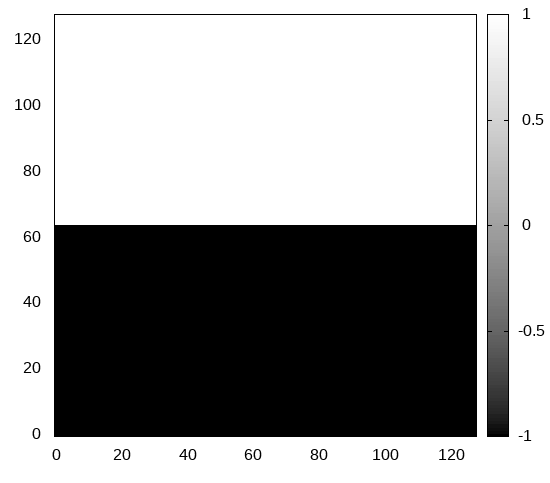
\includegraphics[width=0.45\textwidth]{Imagenes/T-TC05-09.png}}
    \subfigure[Distribución con $T = 0.8K$, $T/T_C \approx 0.89$.]{
        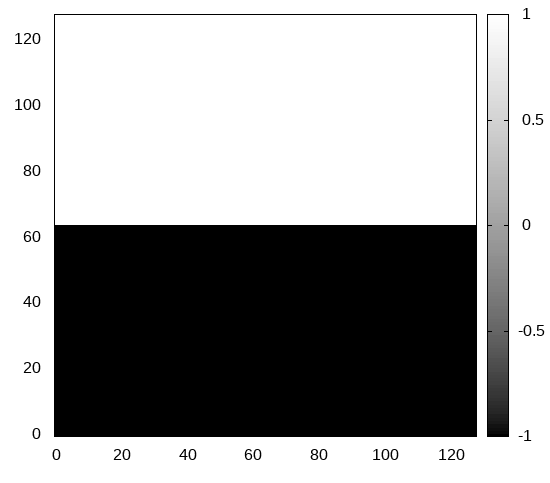
\includegraphics[width=0.45\textwidth]{Imagenes/T-TC05-09.png}}
    \subfigure[Distribución con $T = 0.9K$, $T/T_C = 1$.]{
        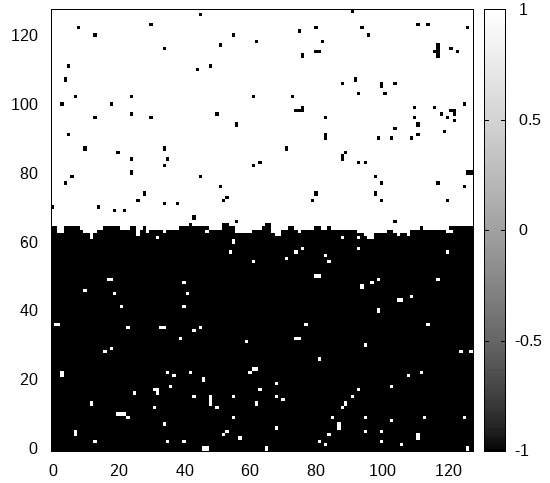
\includegraphics[width=0.45\textwidth]{Imagenes/T-TC08-09.png}}
    \subfigure[Distribución con $T = 0.95K$, $T/T_C \approx 1.06$.]{
        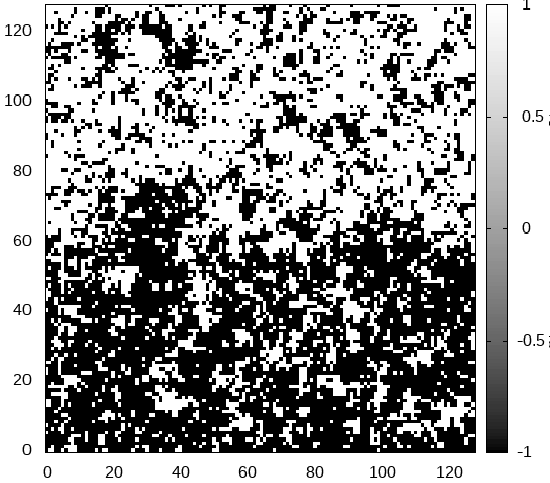
\includegraphics[width=0.45\textwidth]{Imagenes/T-TC095-09.png}}  
    \subfigure[Distribución con $T = 1K$, $T/T_C \approx 1.11$.]{
        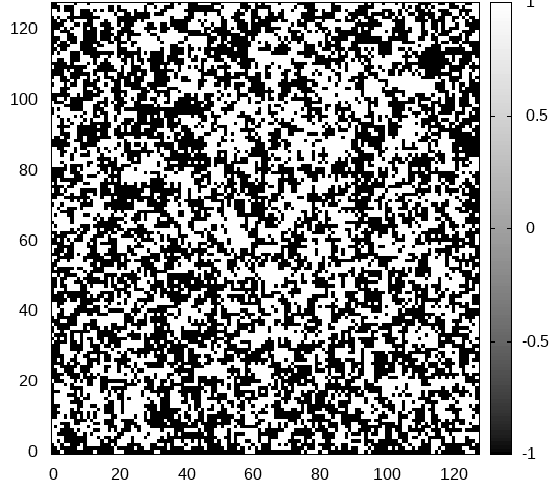
\includegraphics[width=0.45\textwidth]{Imagenes/T-TC1-09.png}} 
    \subfigure[Prueba distribución con $T = 0.9K$, tras aproximadamente 10000 pasos Montecarlo.]{
        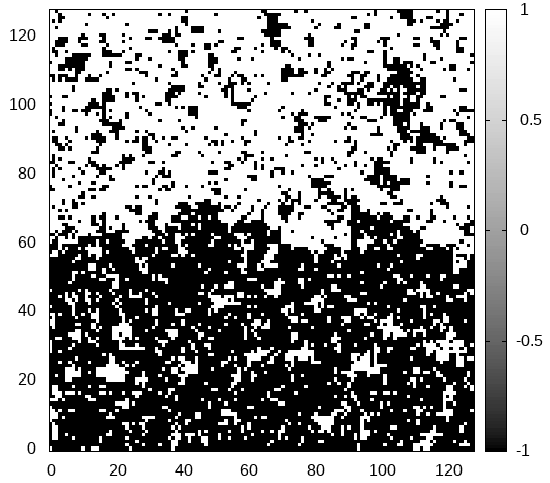
\includegraphics[width=0.45\textwidth]{Imagenes/TC10k.png}}     
    
  \end{center}
\end{figure}\\
Por esta misma razón vamos a concluir que $T_C \approx 0.9K$ y el resto de apartados los ejemplos van a tratar sobre $T = 0.5K, \hspace{1mm} 0.8K \hspace{1mm}, T_C, \hspace{1mm} y \hspace{1mm} 1K$.

\subsubsection{Magnetización y Energía.}
Para este caso, se han realizado la obtención de datos para las temperaturas previamente descritas y para un mayor número de pasos Montecarlo: 2500 para todos los casos. En este caso para $x=0.9$ se han realizado las gráficas de tal forma que la suma total de magnetizaciones por dominios sea el $<M>$ real, es decir, se ha considerado que $<M>$ en el dominio de -1 es positivo y al revés en el +1. Podemos denotar todos lo explicado con anterioridad expresado con diferentes magnitudes así cómo los diferentes matices explicados en diferentes secciones anteriores.\\

Se ha realizado un estudio de $<E(T)>$, y de $<M(T)>$. Este último por dominios y por cortes en el eje y.\\

Igual que en el anterior apartado. Debido al gran tamaño de las imágenes, la gran cantidad de datos y a las limitaciones del documento es imposible ver las imágenes con denótale claridad, por esta misma razón haciendo clic en el siguiente enlace se pueden ver todas las imágenes de este trabajo con mucha mayor claridad: {\underline{\href{https://drive.google.com/drive/folders/1ivzNfi-jLKLyxUTFhOSw3gwLT2m2QSXb?usp=sharing}{gráficas con mucha mayor resolución}}}.

\begin{figure}[H]
  \begin{center}        
    \caption{Variaciones de la energía ($<E(T)>$) para diferentes temperaturas $(T)$, diferentes magnetizaciones ($m$) y diferentes número de partículas ($N$).}
    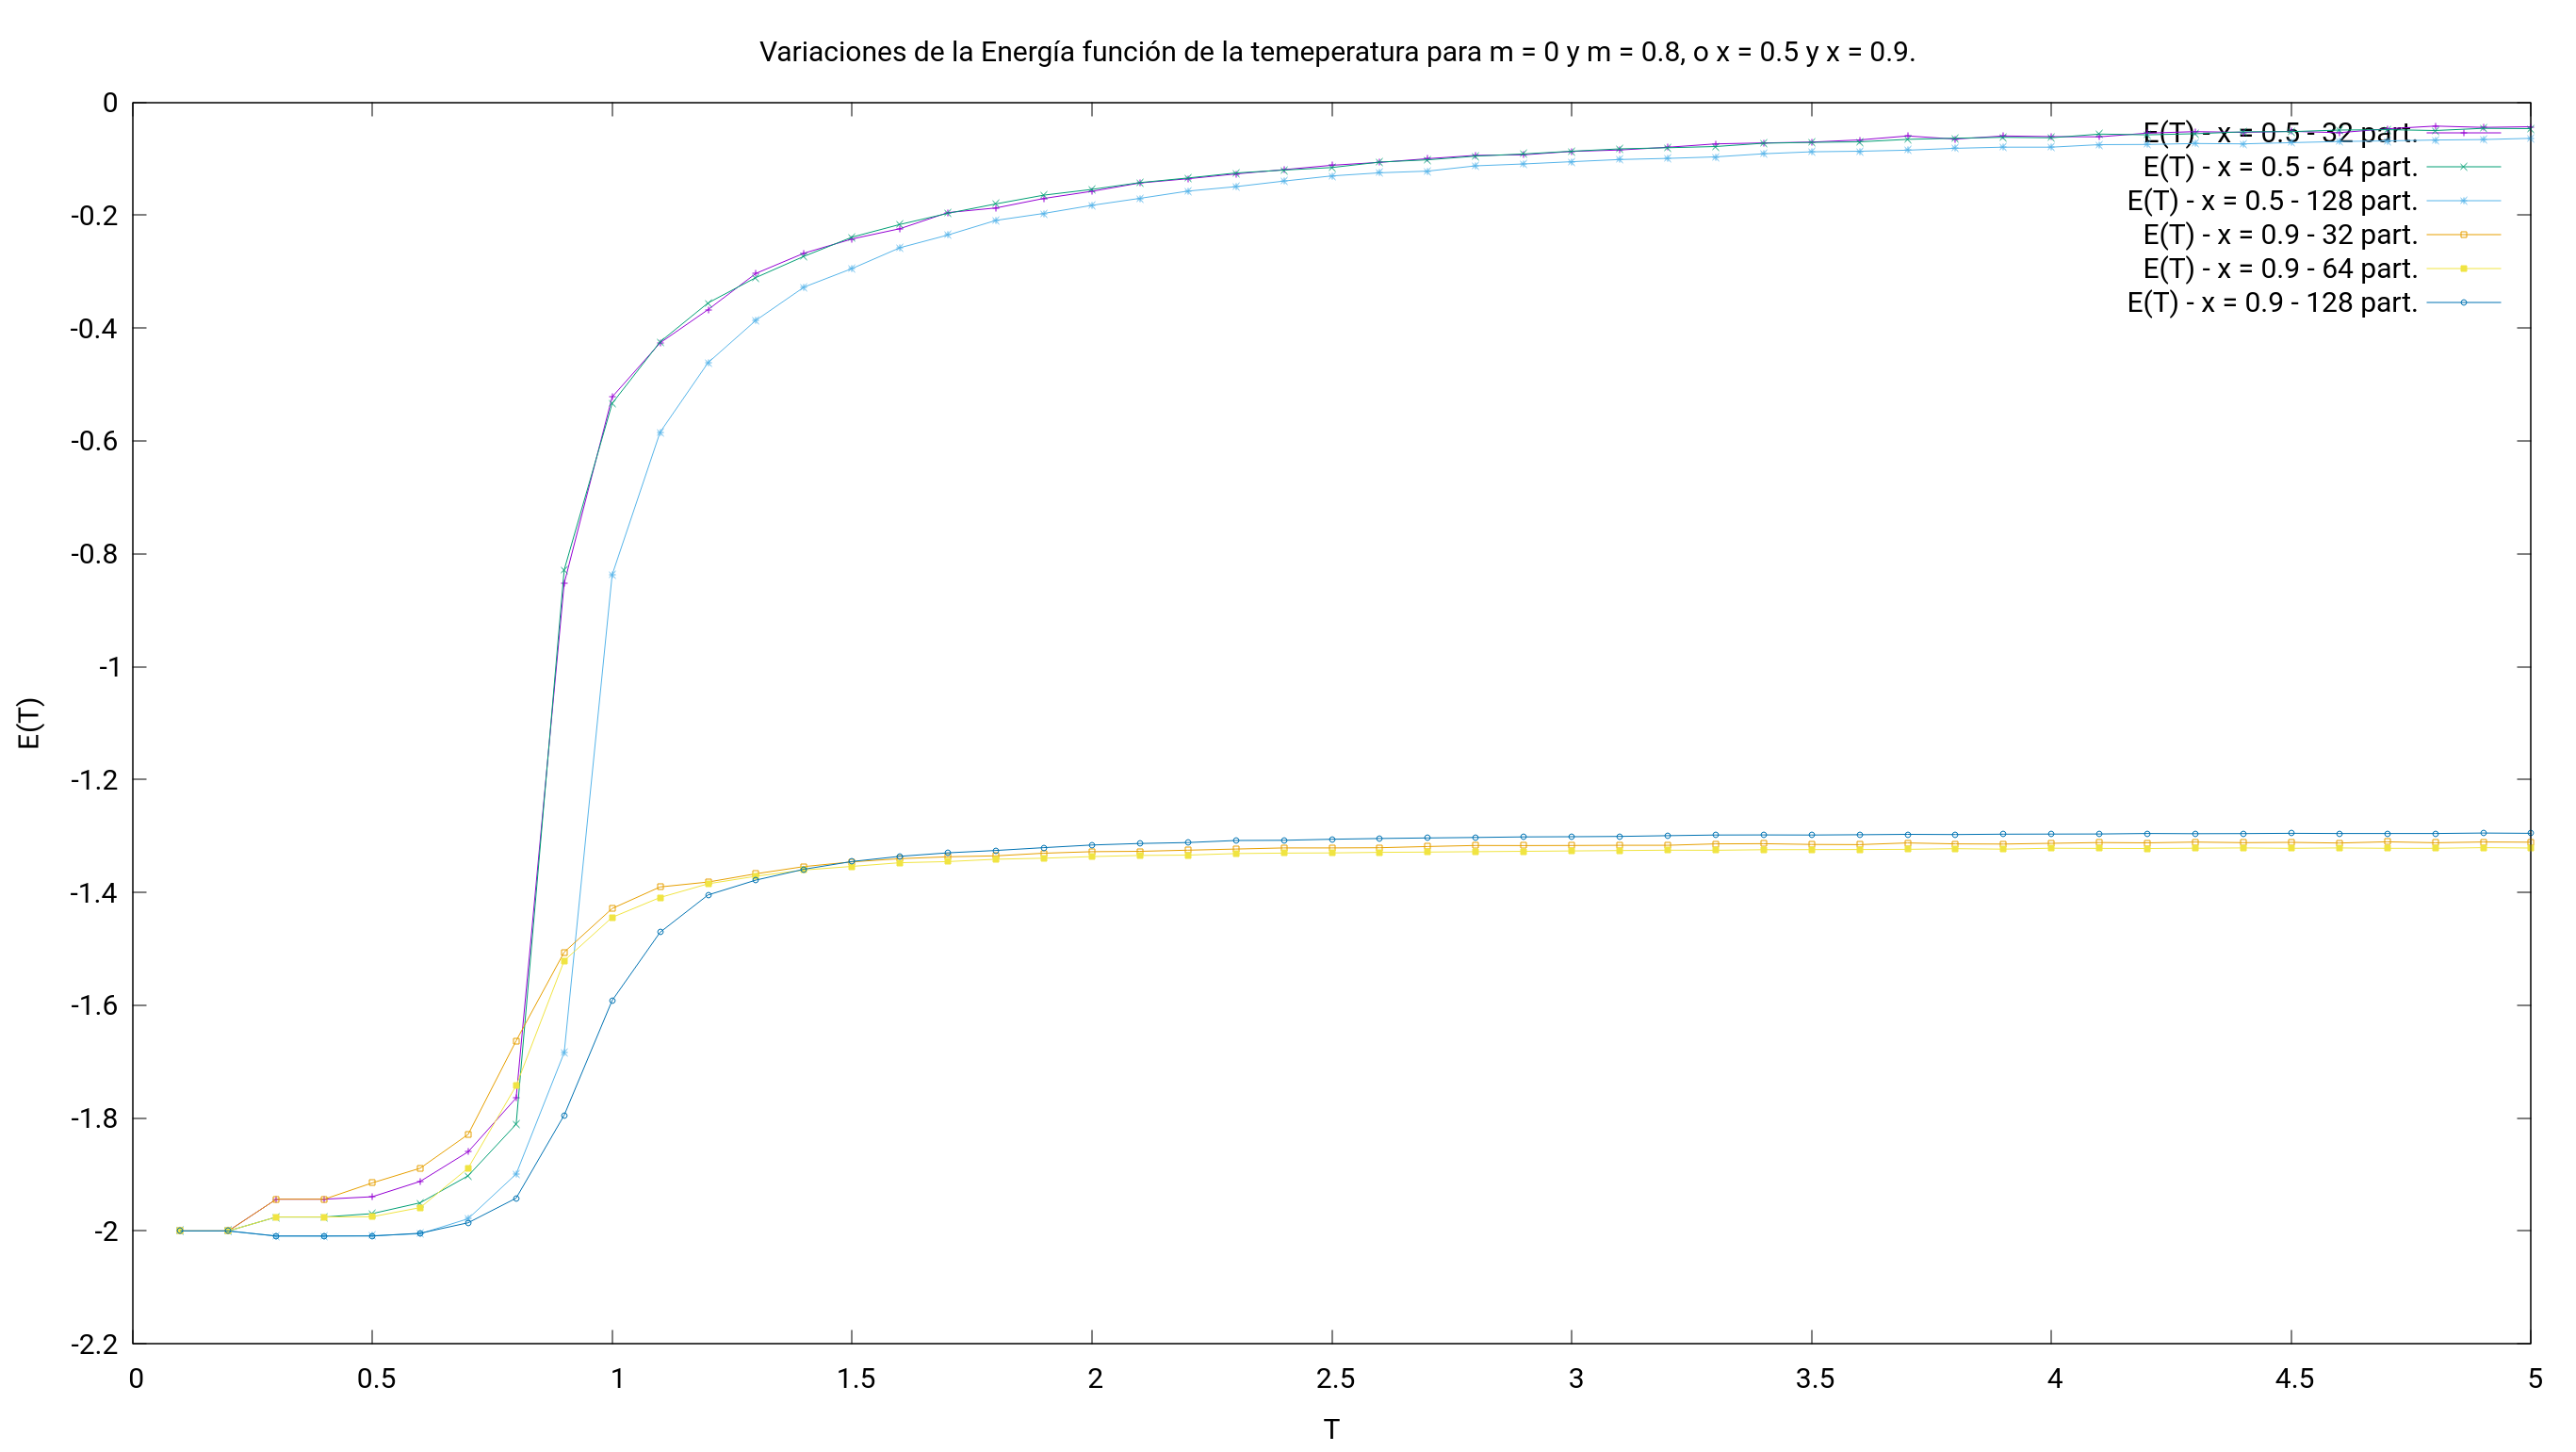
\includegraphics[width=1.1\textwidth]{Imagenes/E(T).png}}     
  \end{center}
\end{figure}\\

\begin{figure}[H]
  \begin{center}        
    \caption{Variaciones de la magnetización ($<M(T)>$) en cortes del eje y para diferentes temperaturas $(T)$, $x=0.5$ y $N=128$x$128$.}
    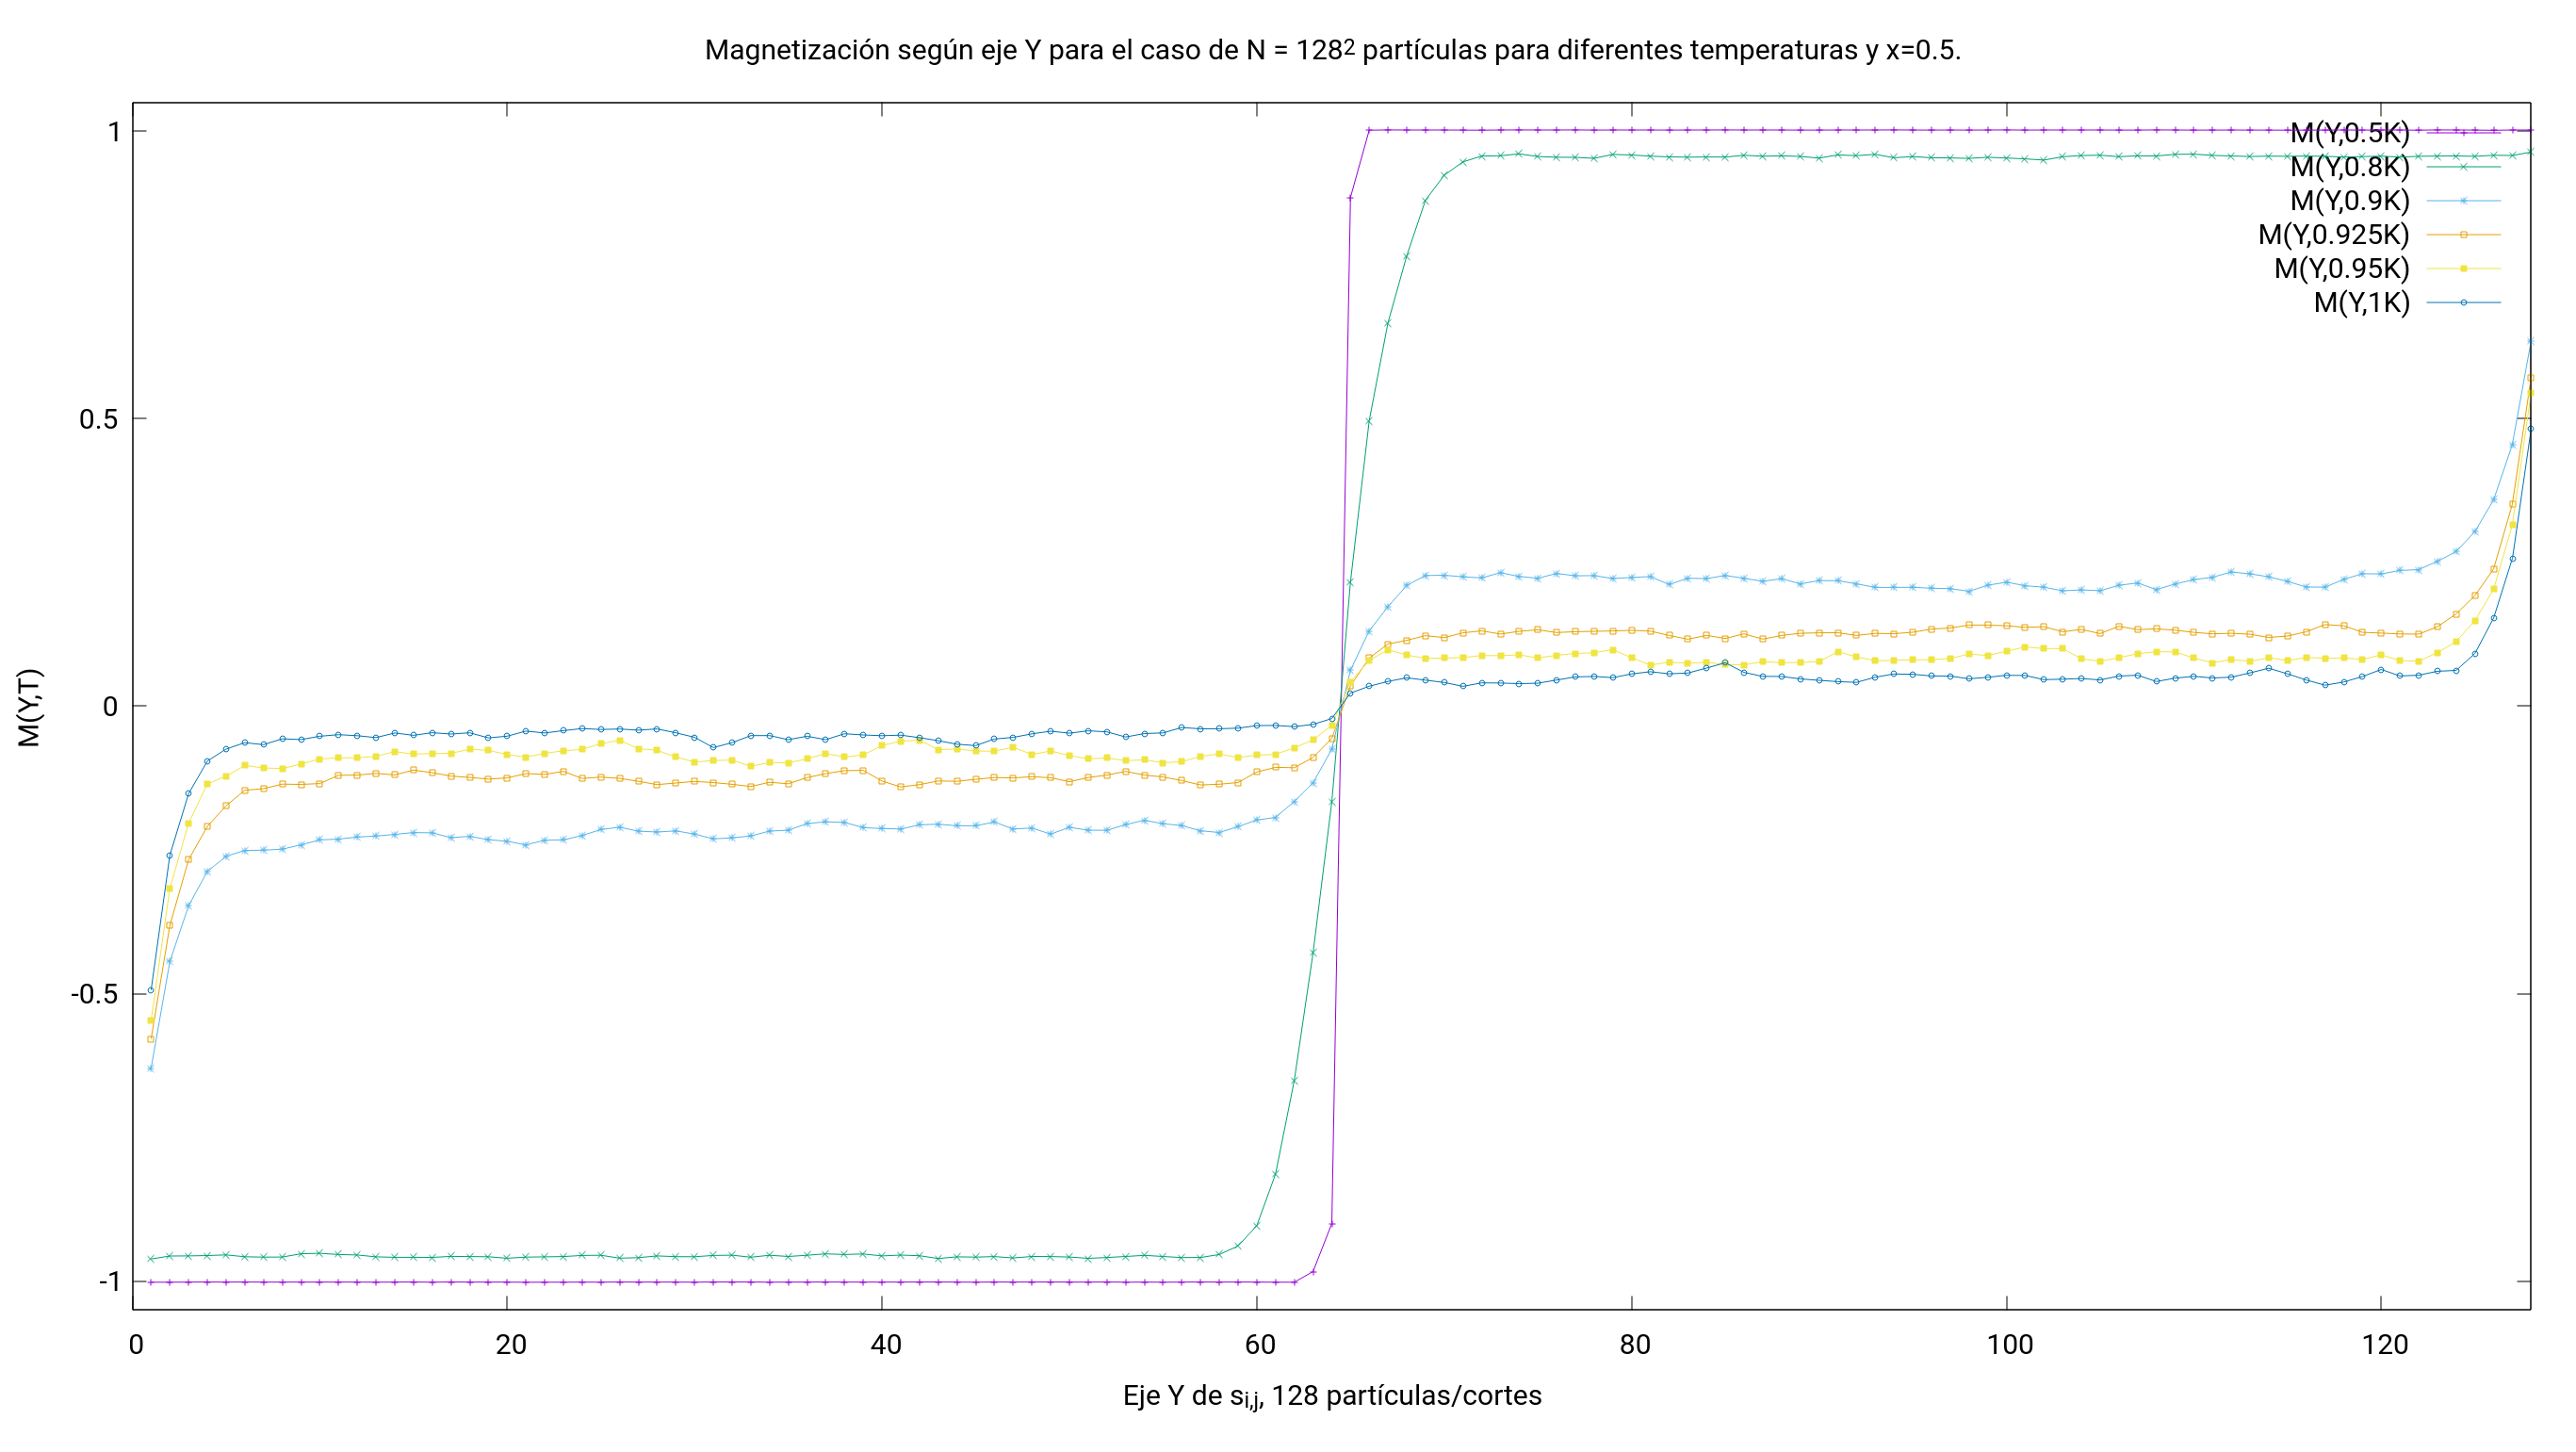
\includegraphics[width=1.1\textwidth]{Imagenes/MagY128X50.png}}     
  \end{center}
\end{figure}\\

\begin{figure}[H]
  \begin{center}        
    \caption{Variaciones de la magnetización ($<M(T)>$) en cortes del eje y para diferentes temperaturas $(T)$, $x=0.9$ y $N=128$x$128$.}
    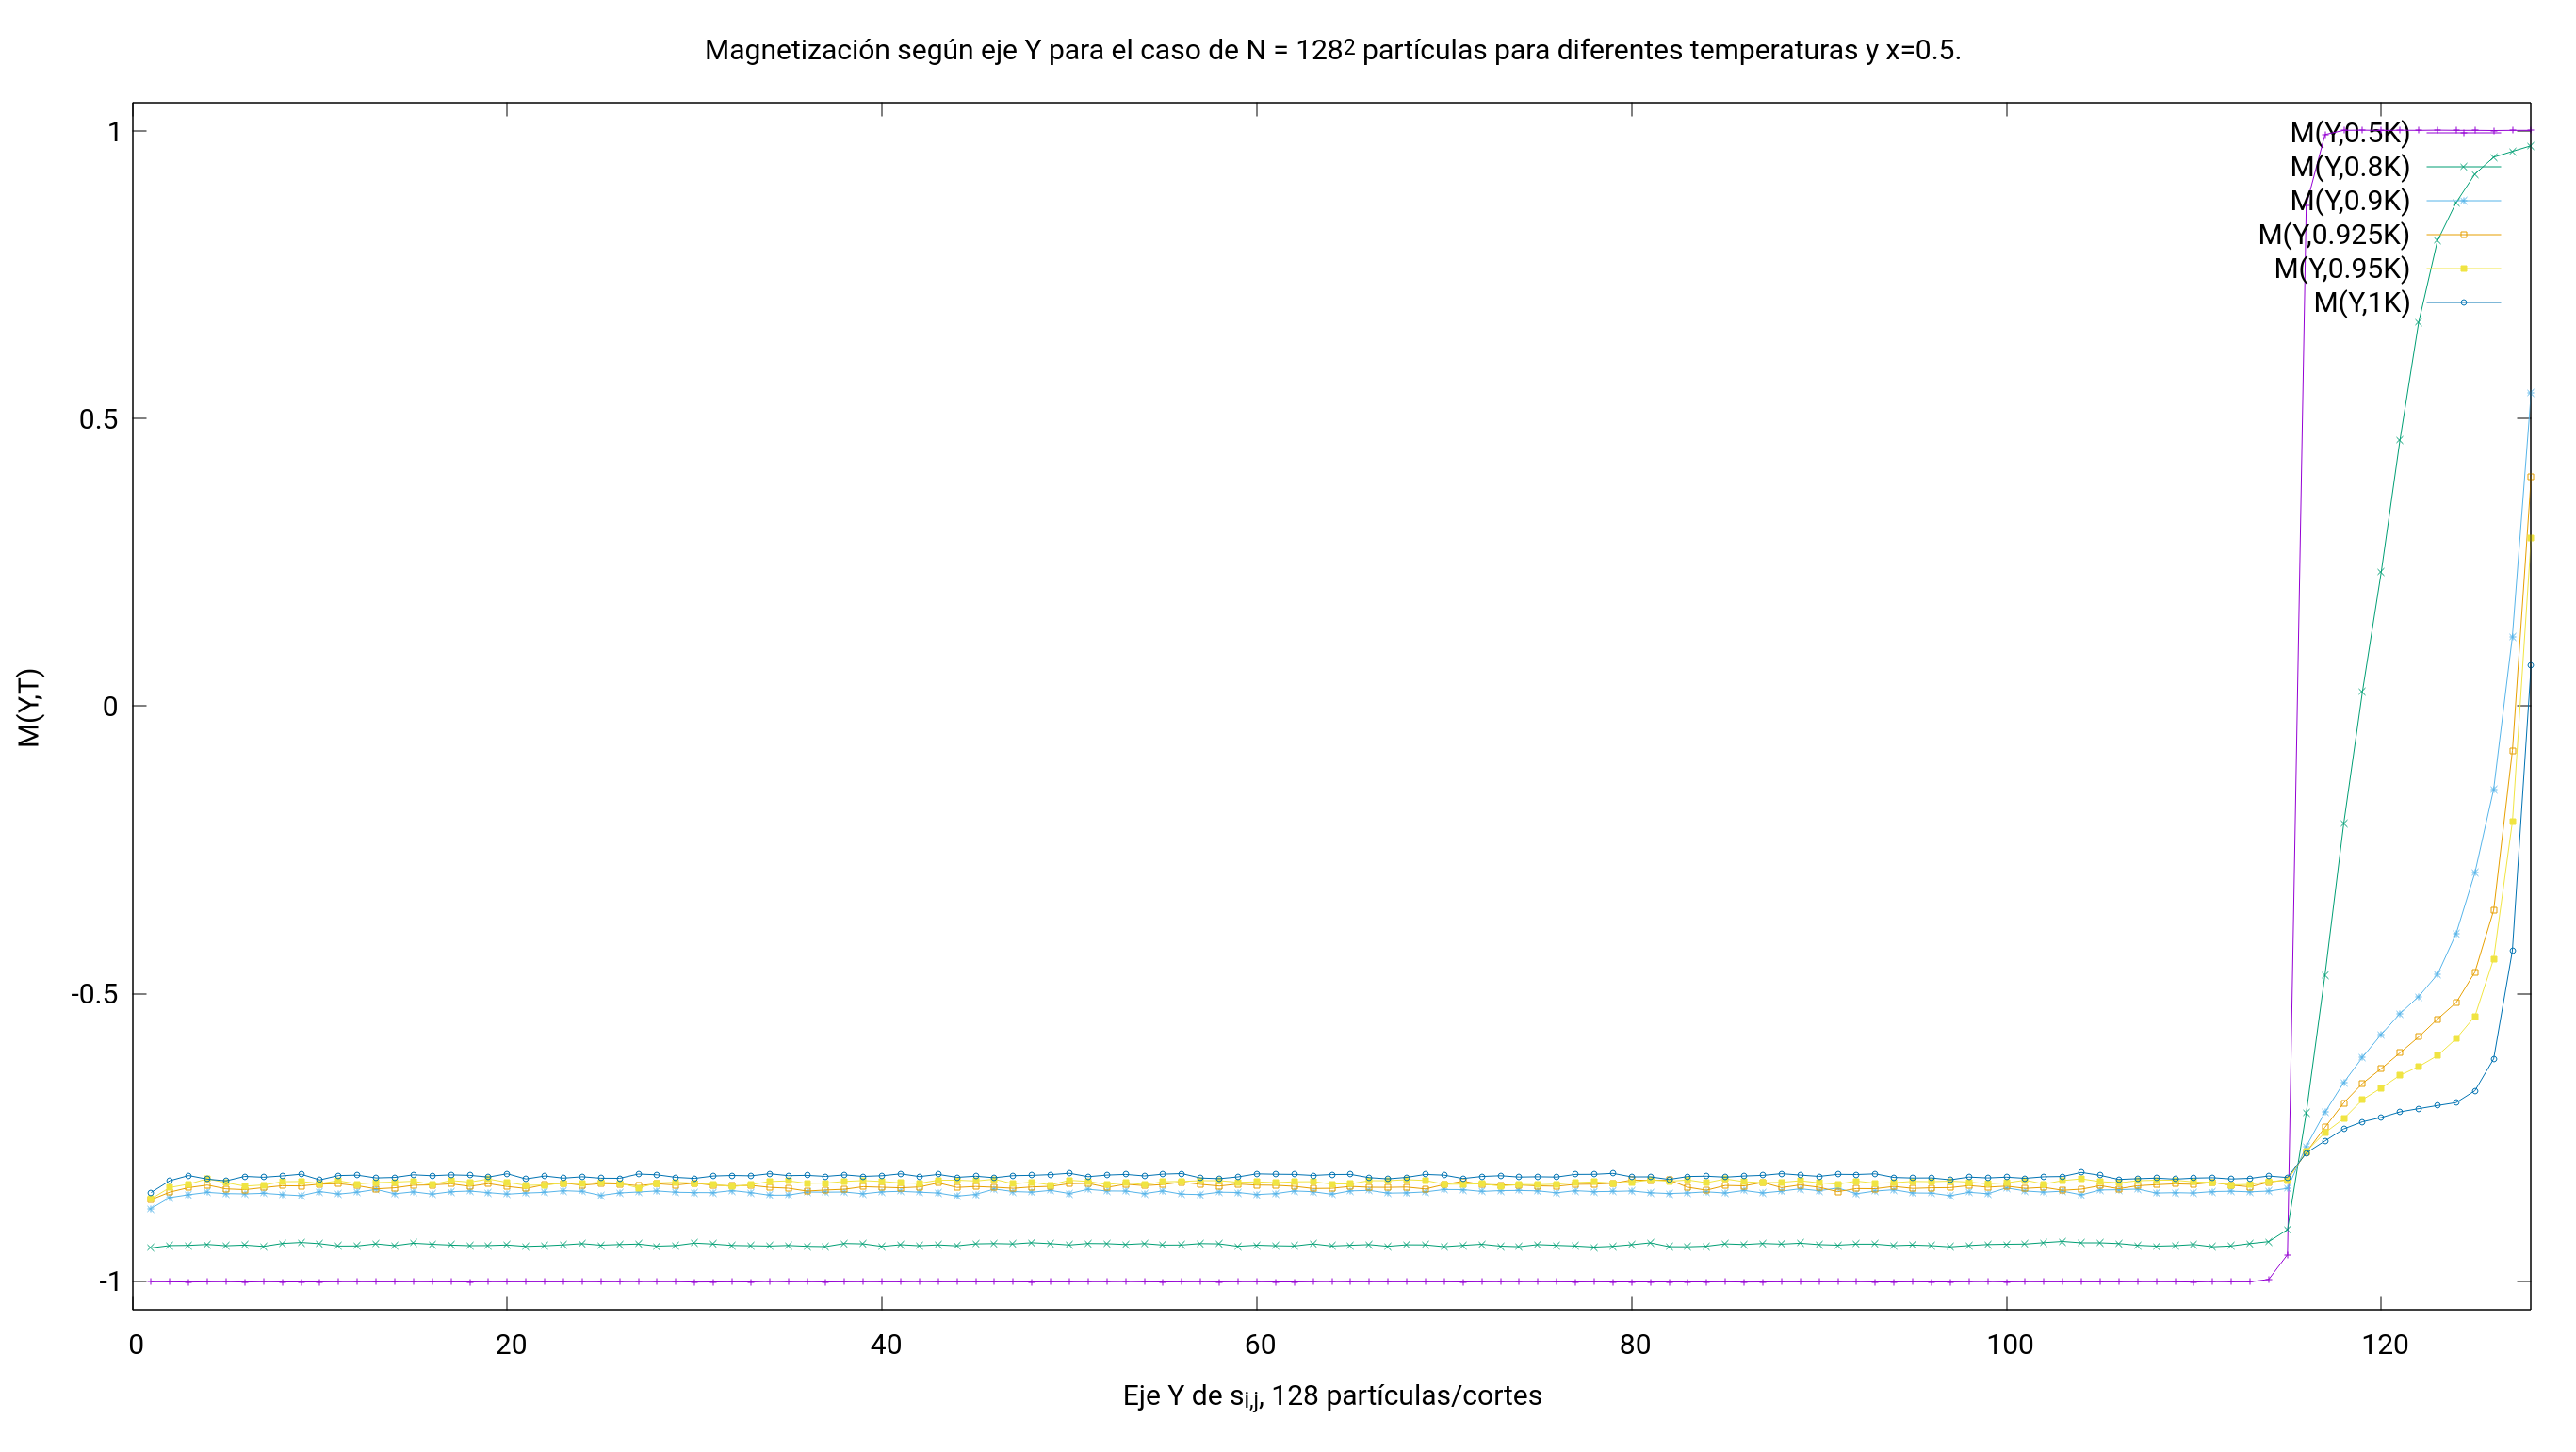
\includegraphics[width=1.1\textwidth]{Imagenes/MagY128X90.png}}     
  \end{center}
\end{figure}\\

\begin{figure}[H]
  \begin{center}        
    \caption{Variaciones de la magnetización ($<M(T)>$) por dominios para diferentes temperaturas $(T)$, $X=0.5$ y $32$x$32$ partículas.}
    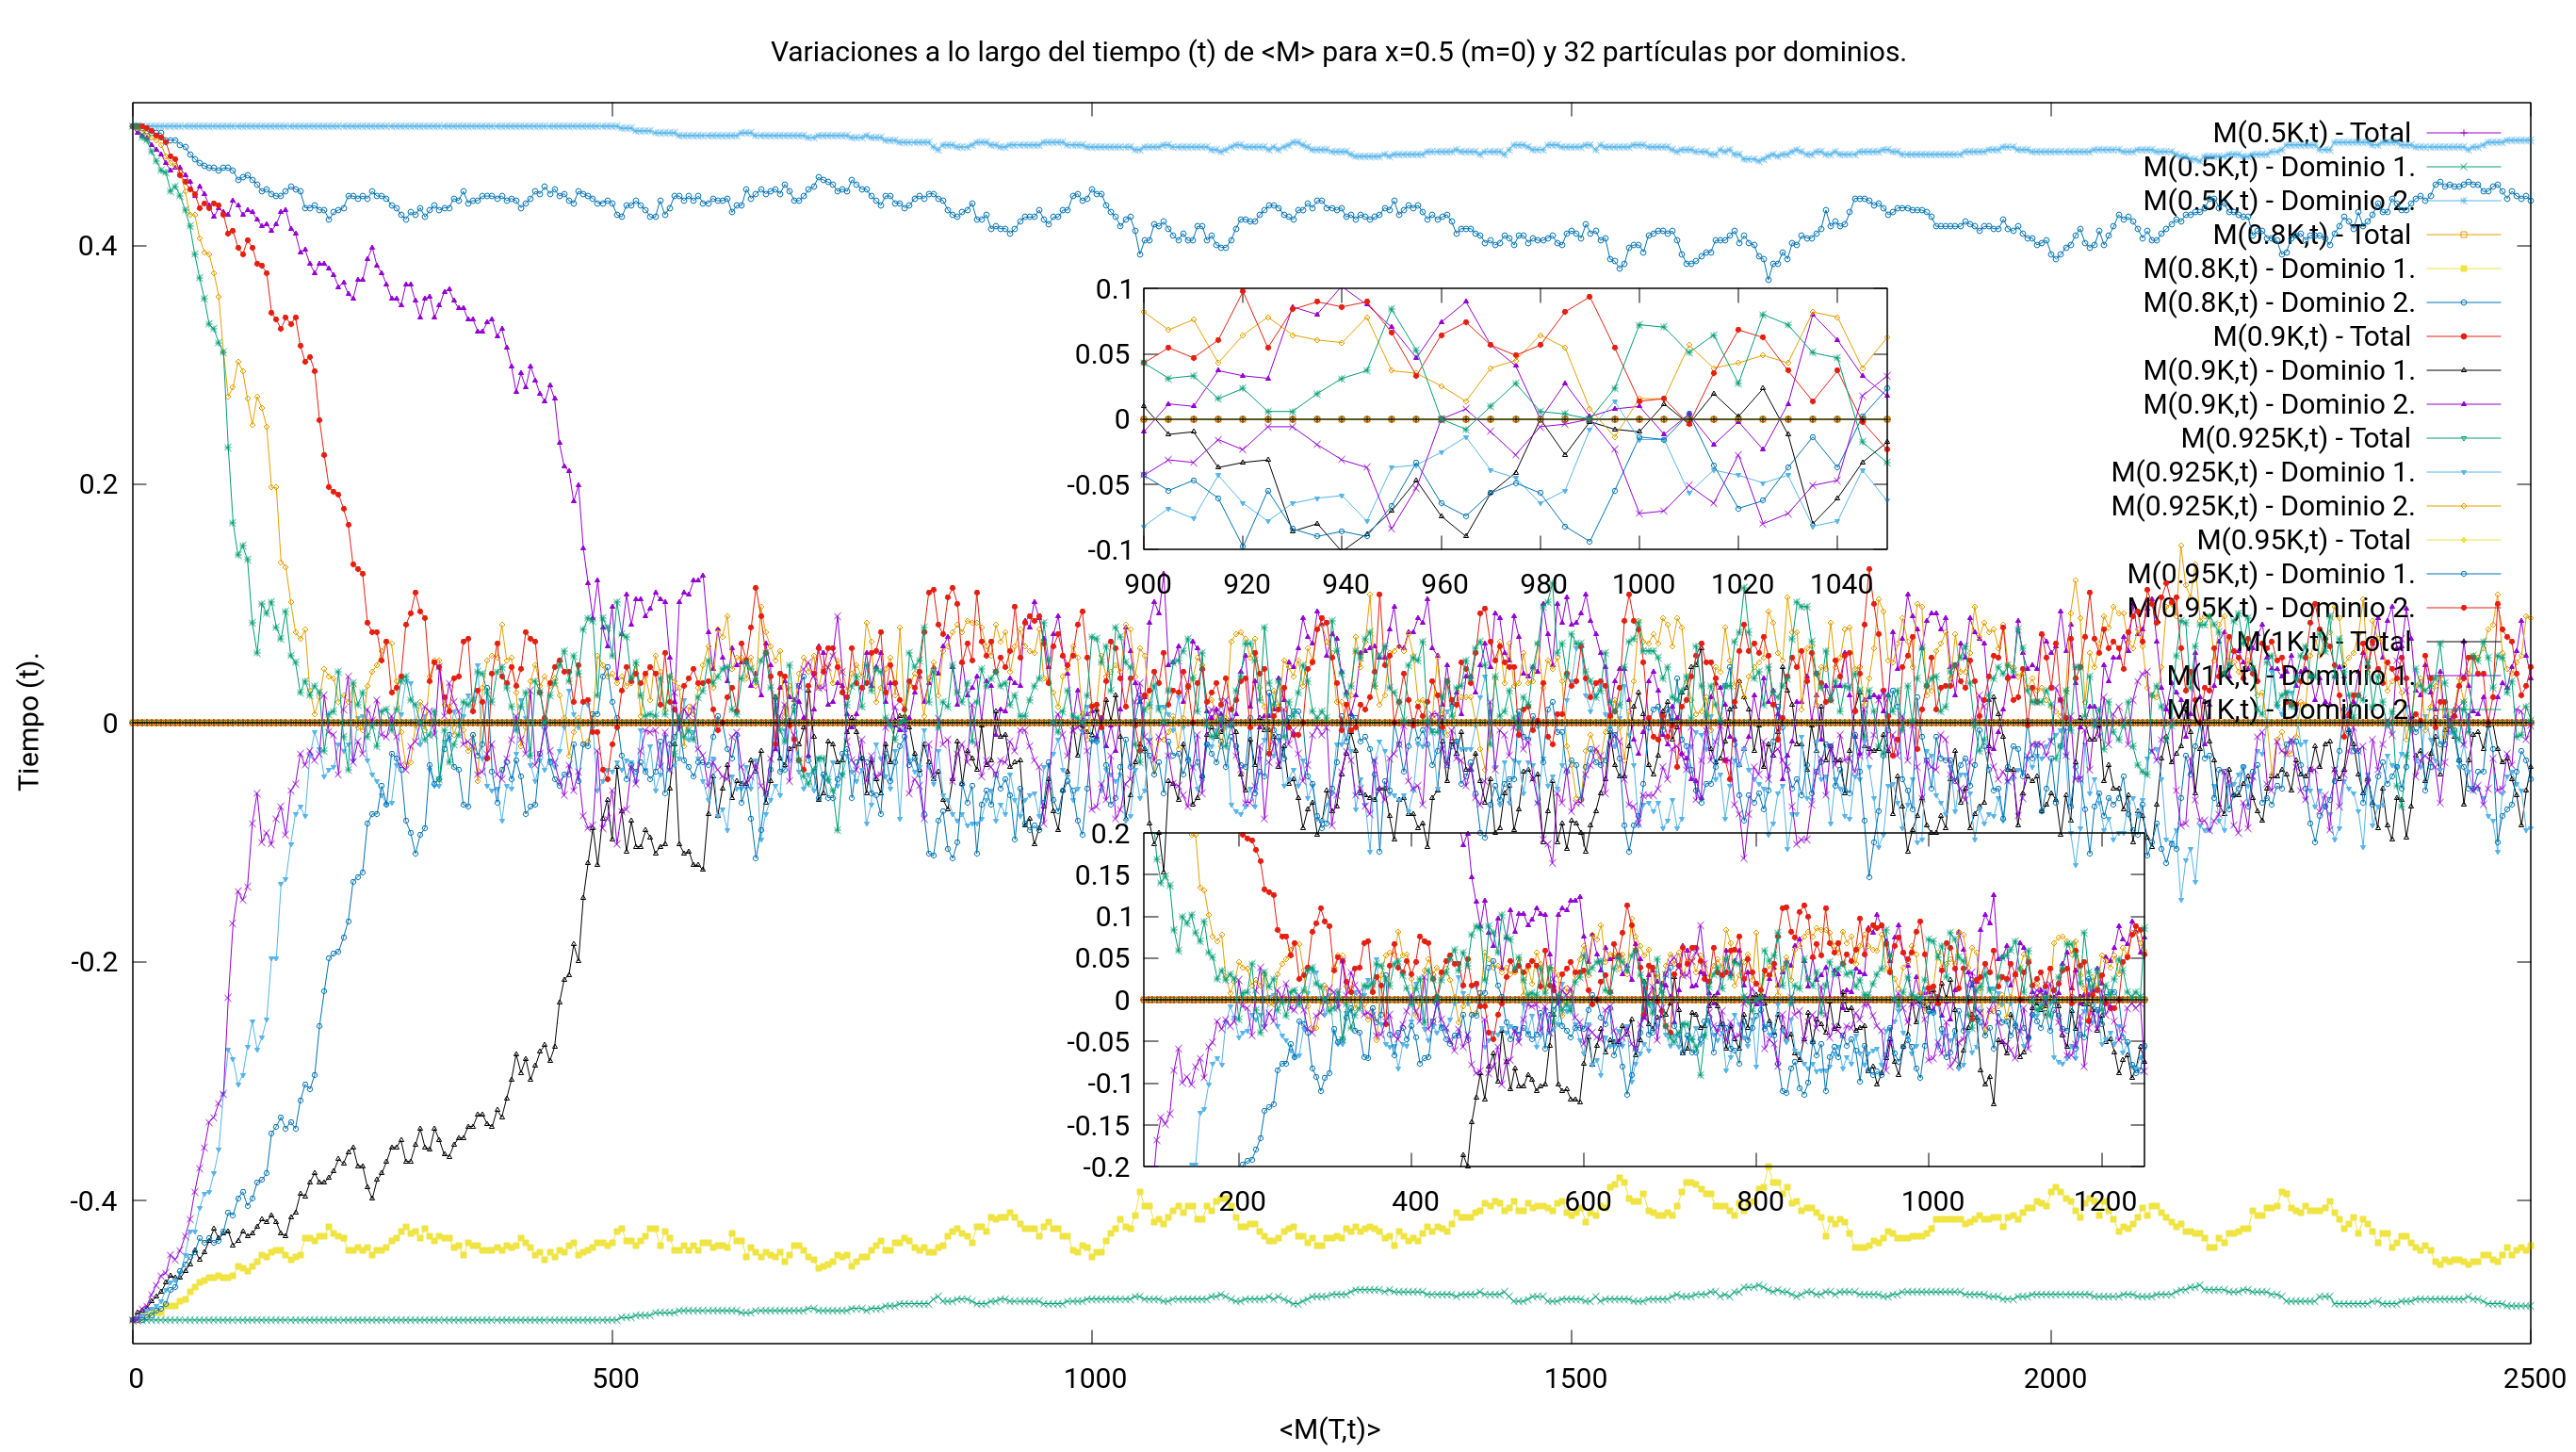
\includegraphics[width=1.1\textwidth]{Imagenes/MagPDom32X50.png}}     
  \end{center}
\end{figure}\\

\begin{figure}[H]
  \begin{center}        
    \caption{Variaciones de la magnetización ($<M(T)>$) por dominios para diferentes temperaturas $(T)$, $X=0.9$ y $32$x$32$ partículas.}
    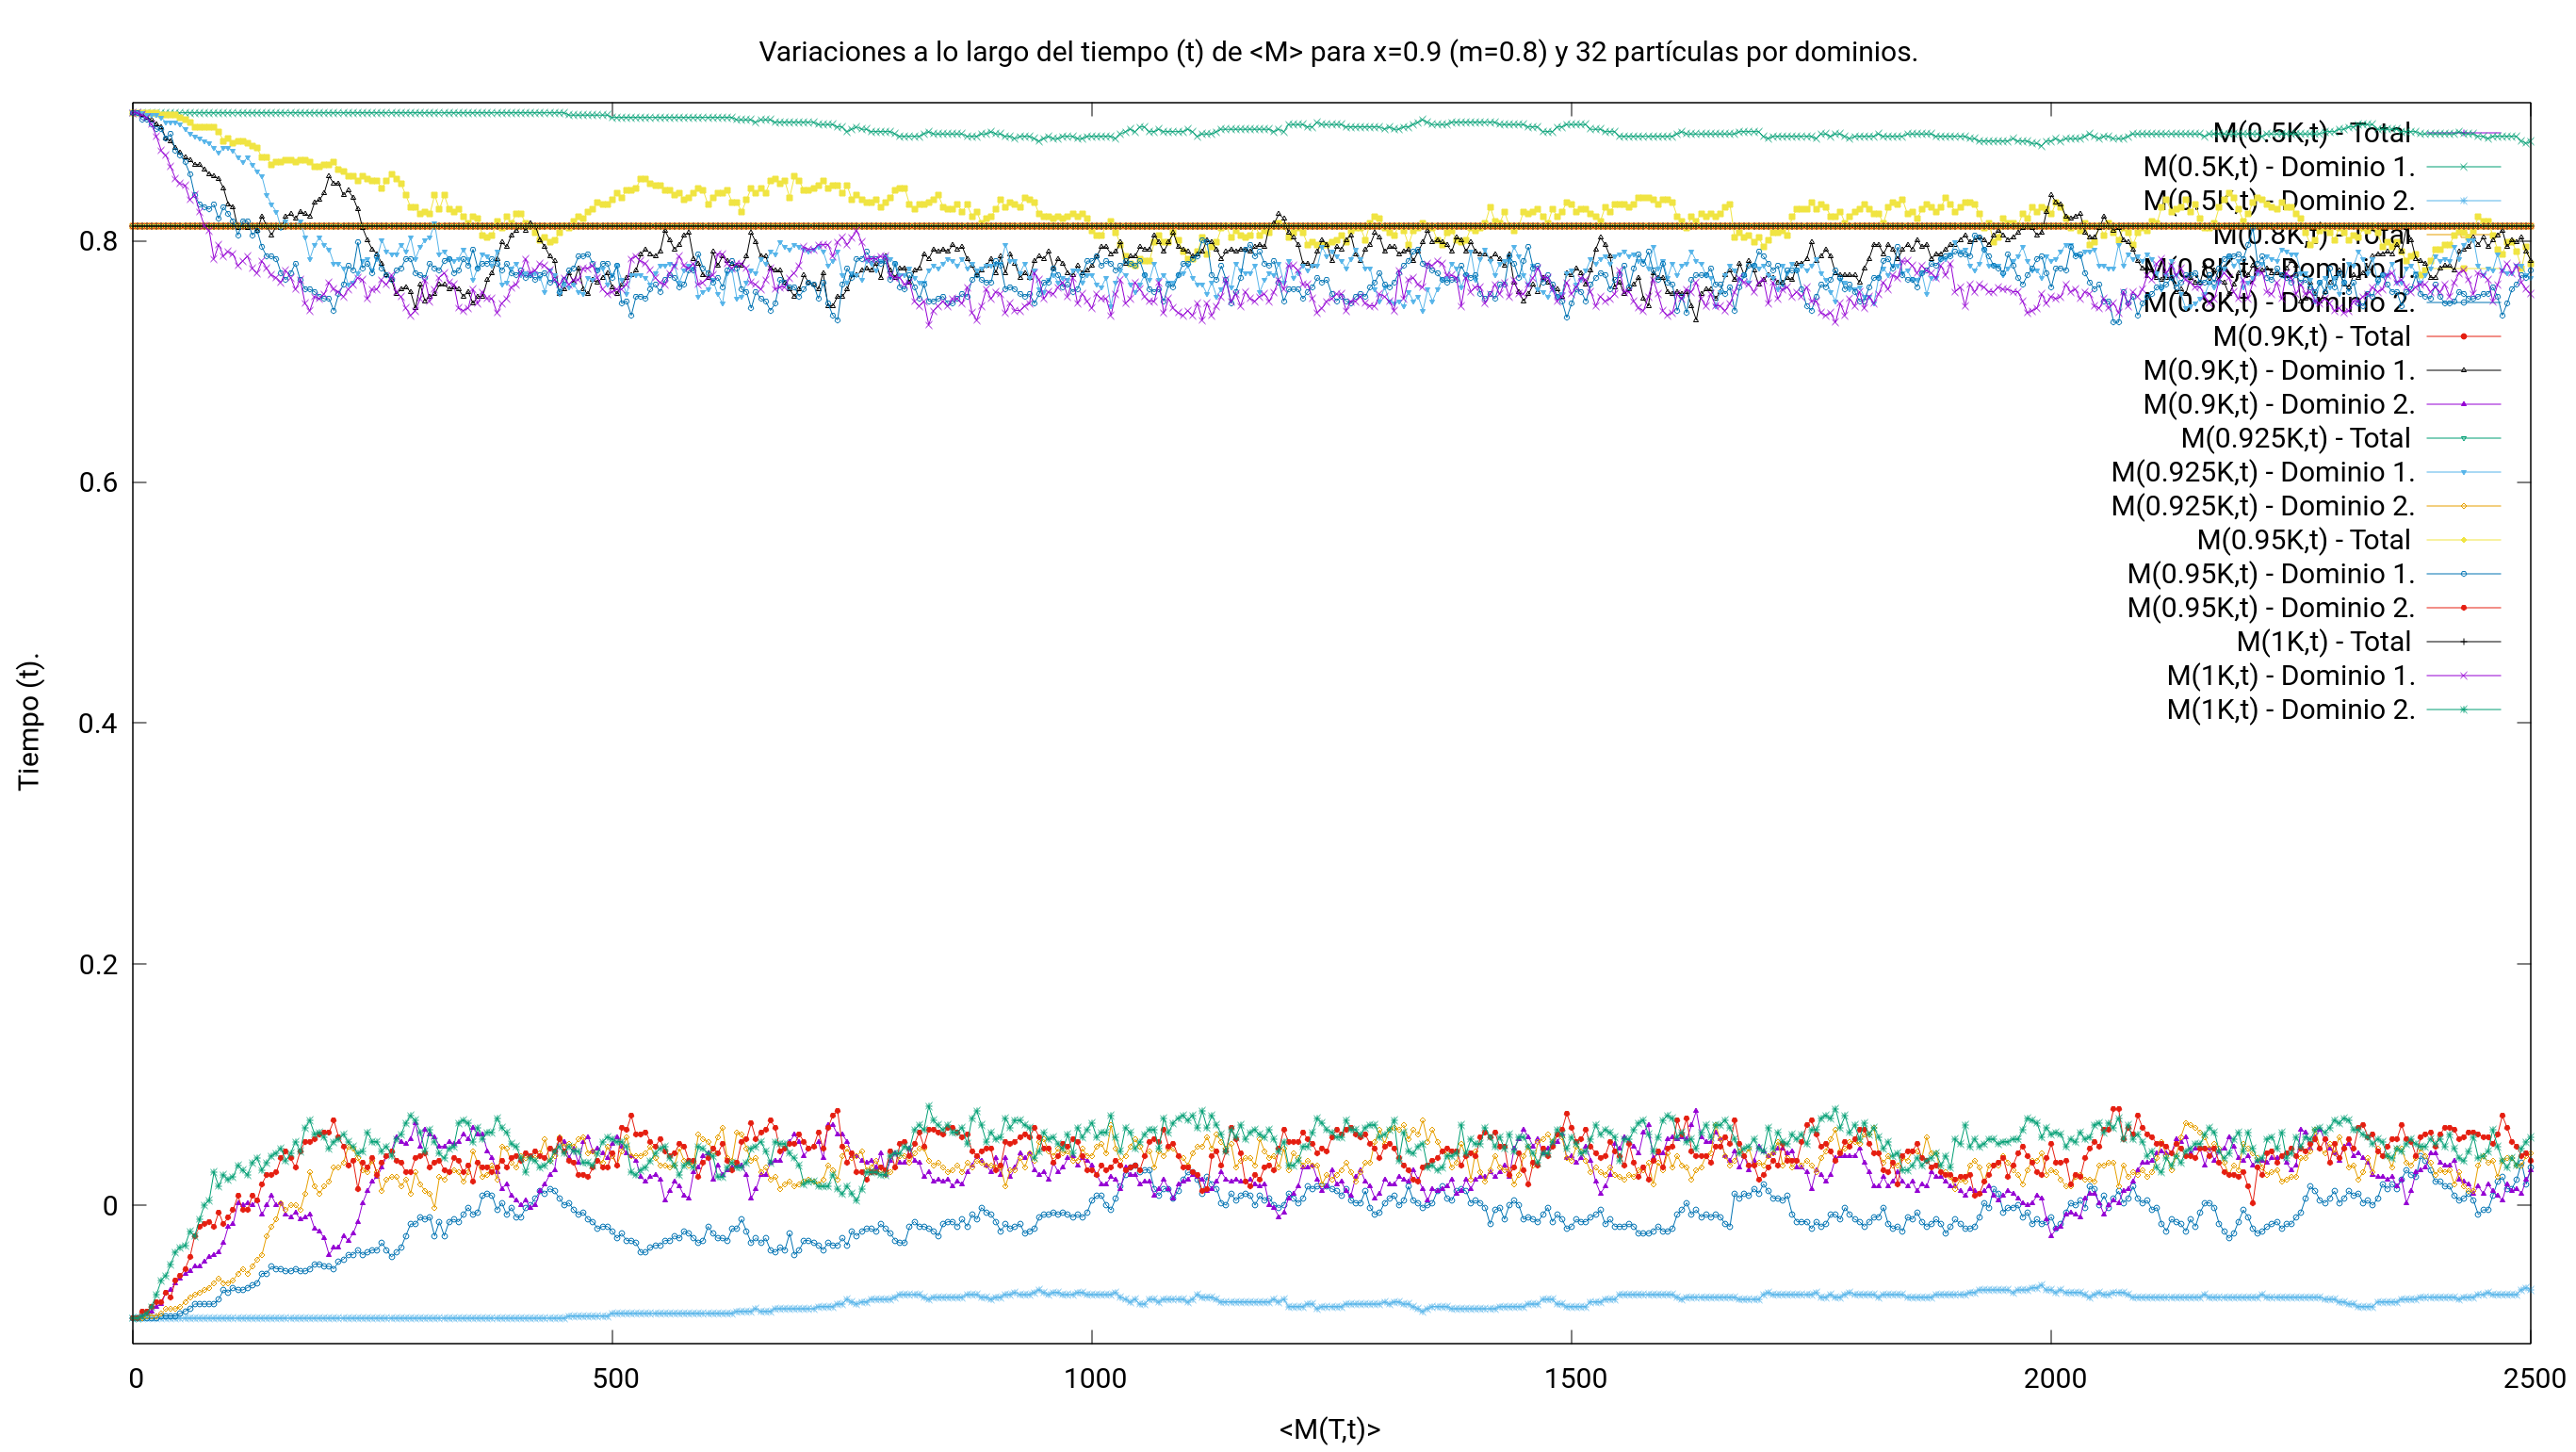
\includegraphics[width=1.1\textwidth]{Imagenes/MagPDom32X90.png}}     
  \end{center}
\end{figure}\\

\begin{figure}[H]
  \begin{center}        
    \caption{Variaciones de la magnetización ($<M(T)>$) por dominios para diferentes temperaturas $(T)$, $X=0.5$ y $64$x$64$ partículas.}
    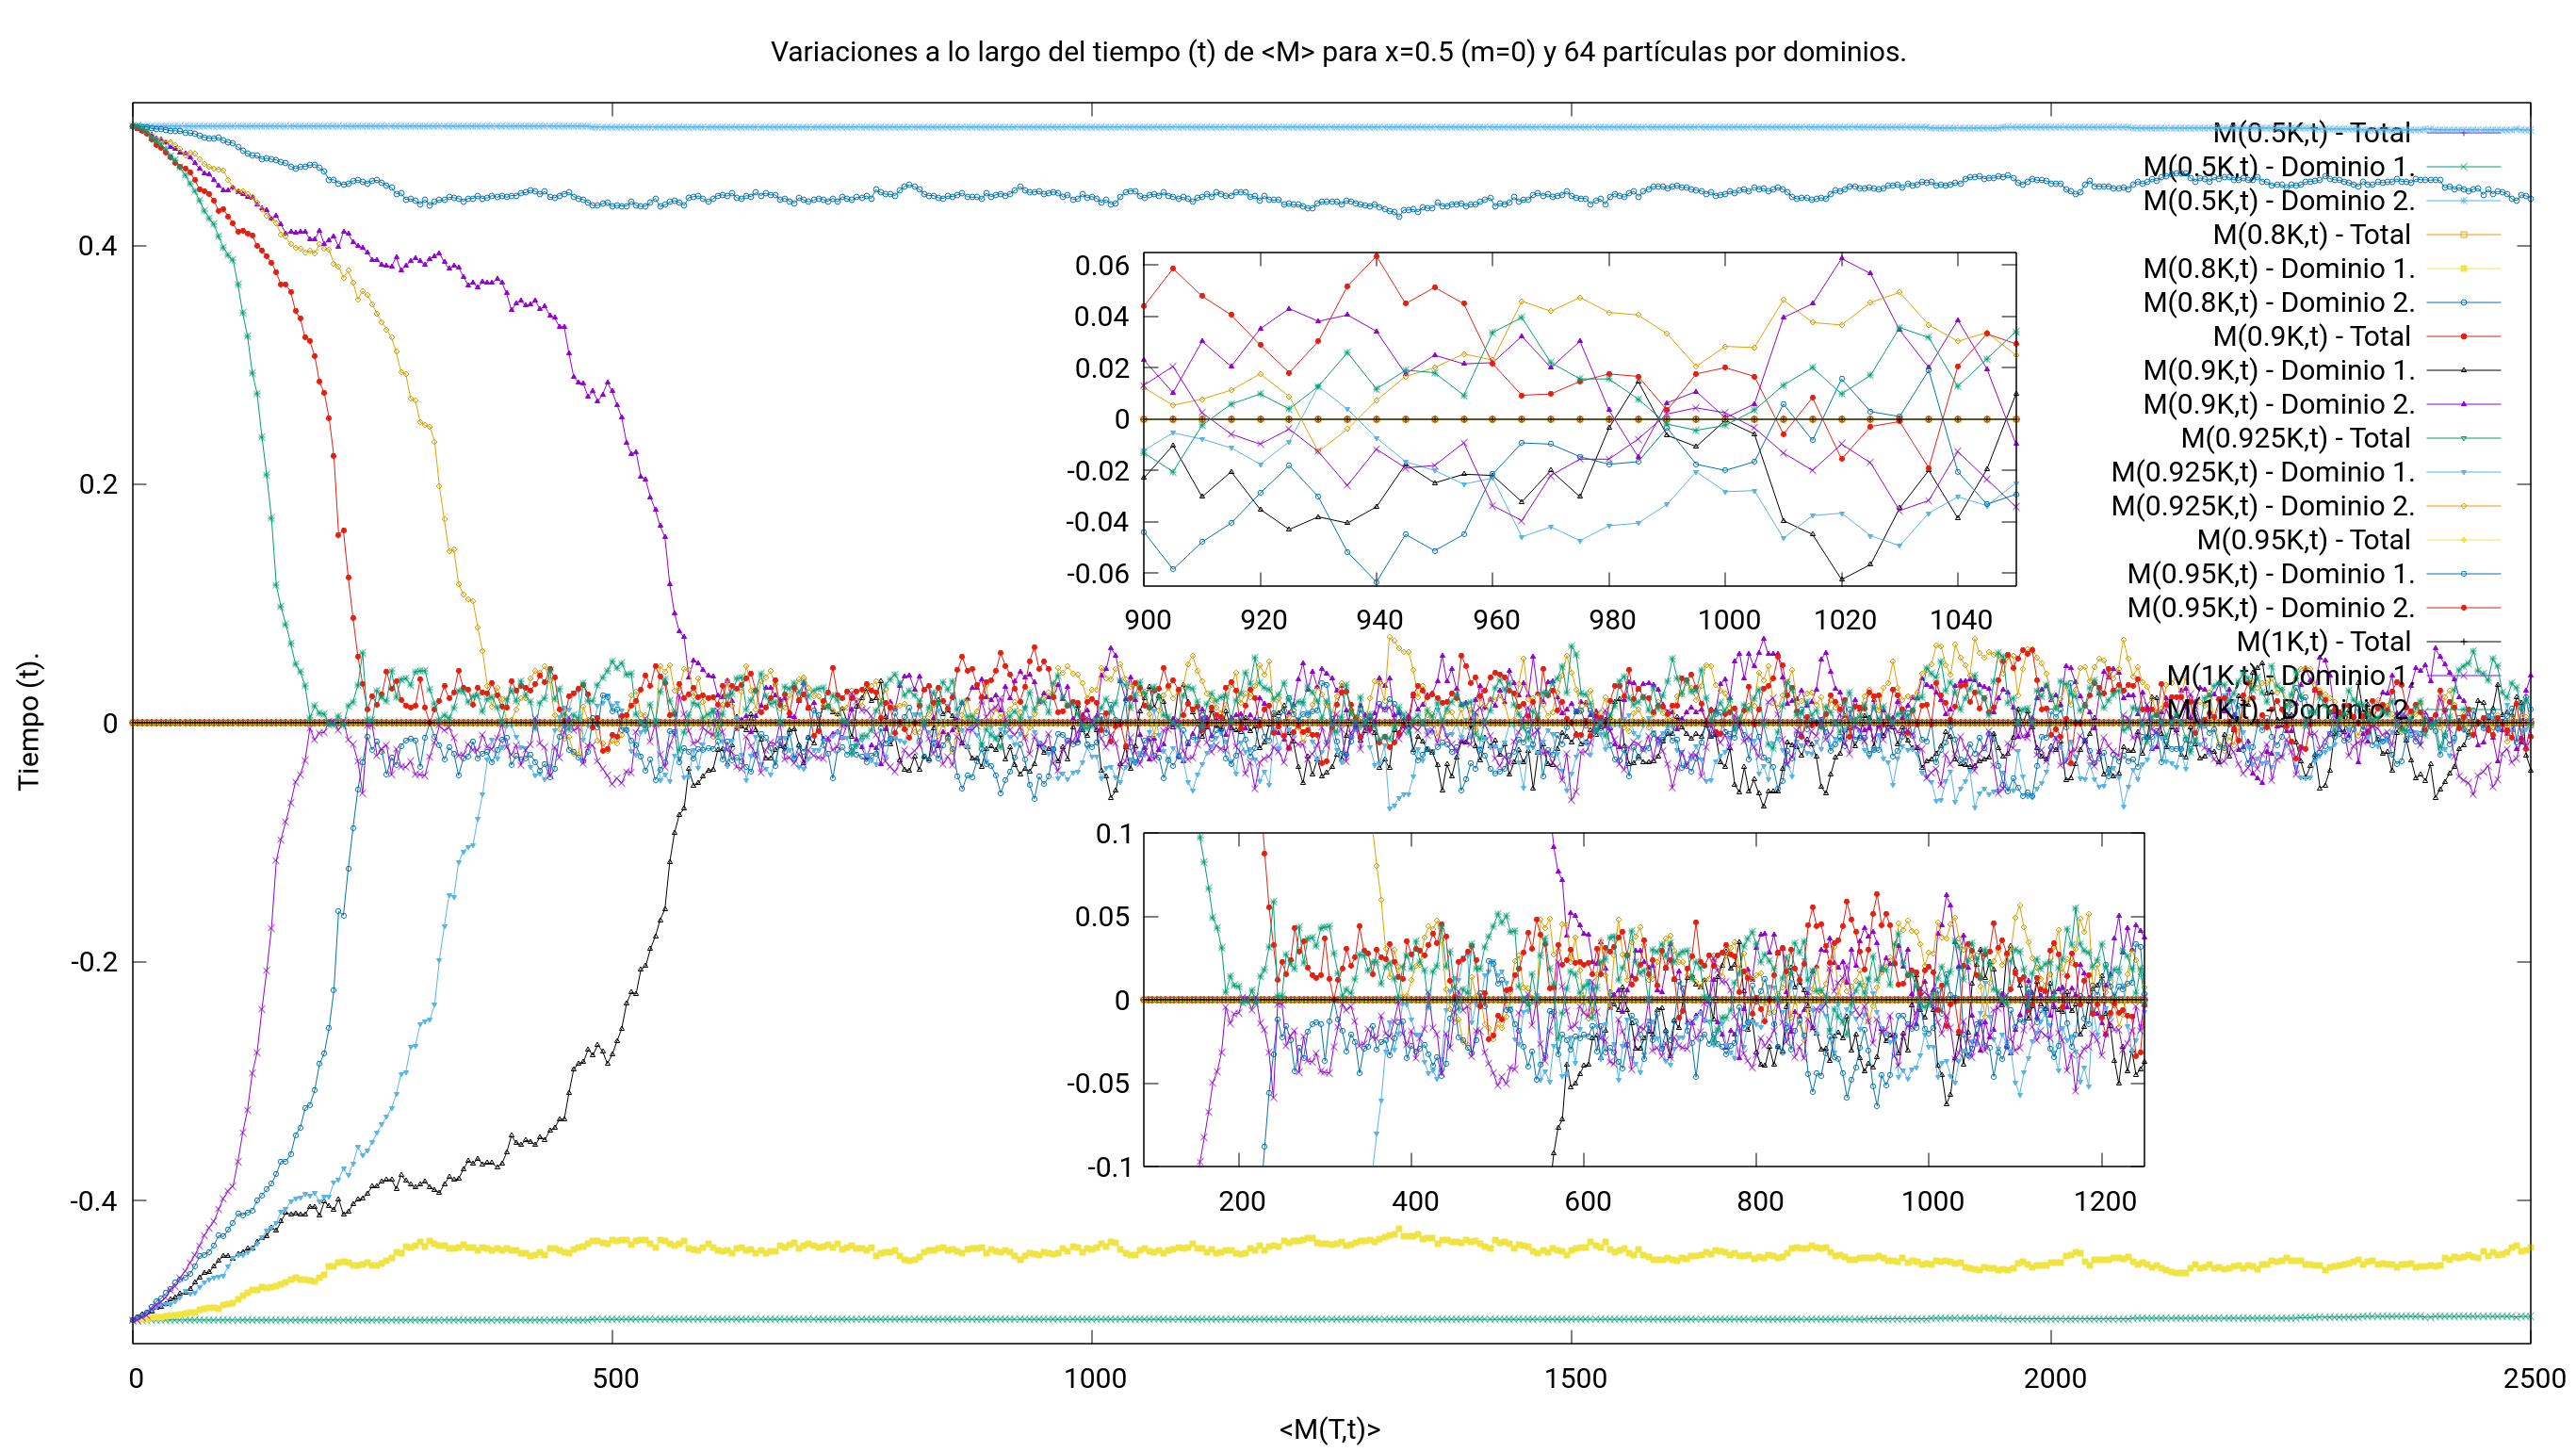
\includegraphics[width=1.1\textwidth]{Imagenes/MagPDom64X50.png}}     
  \end{center}
\end{figure}\\

\begin{figure}[H]
  \begin{center}        
    \caption{Variaciones de la magnetización ($<M(T)>$) por dominios para diferentes temperaturas $(T)$, $X=0.9$ y $64$x$64$ partículas.}
    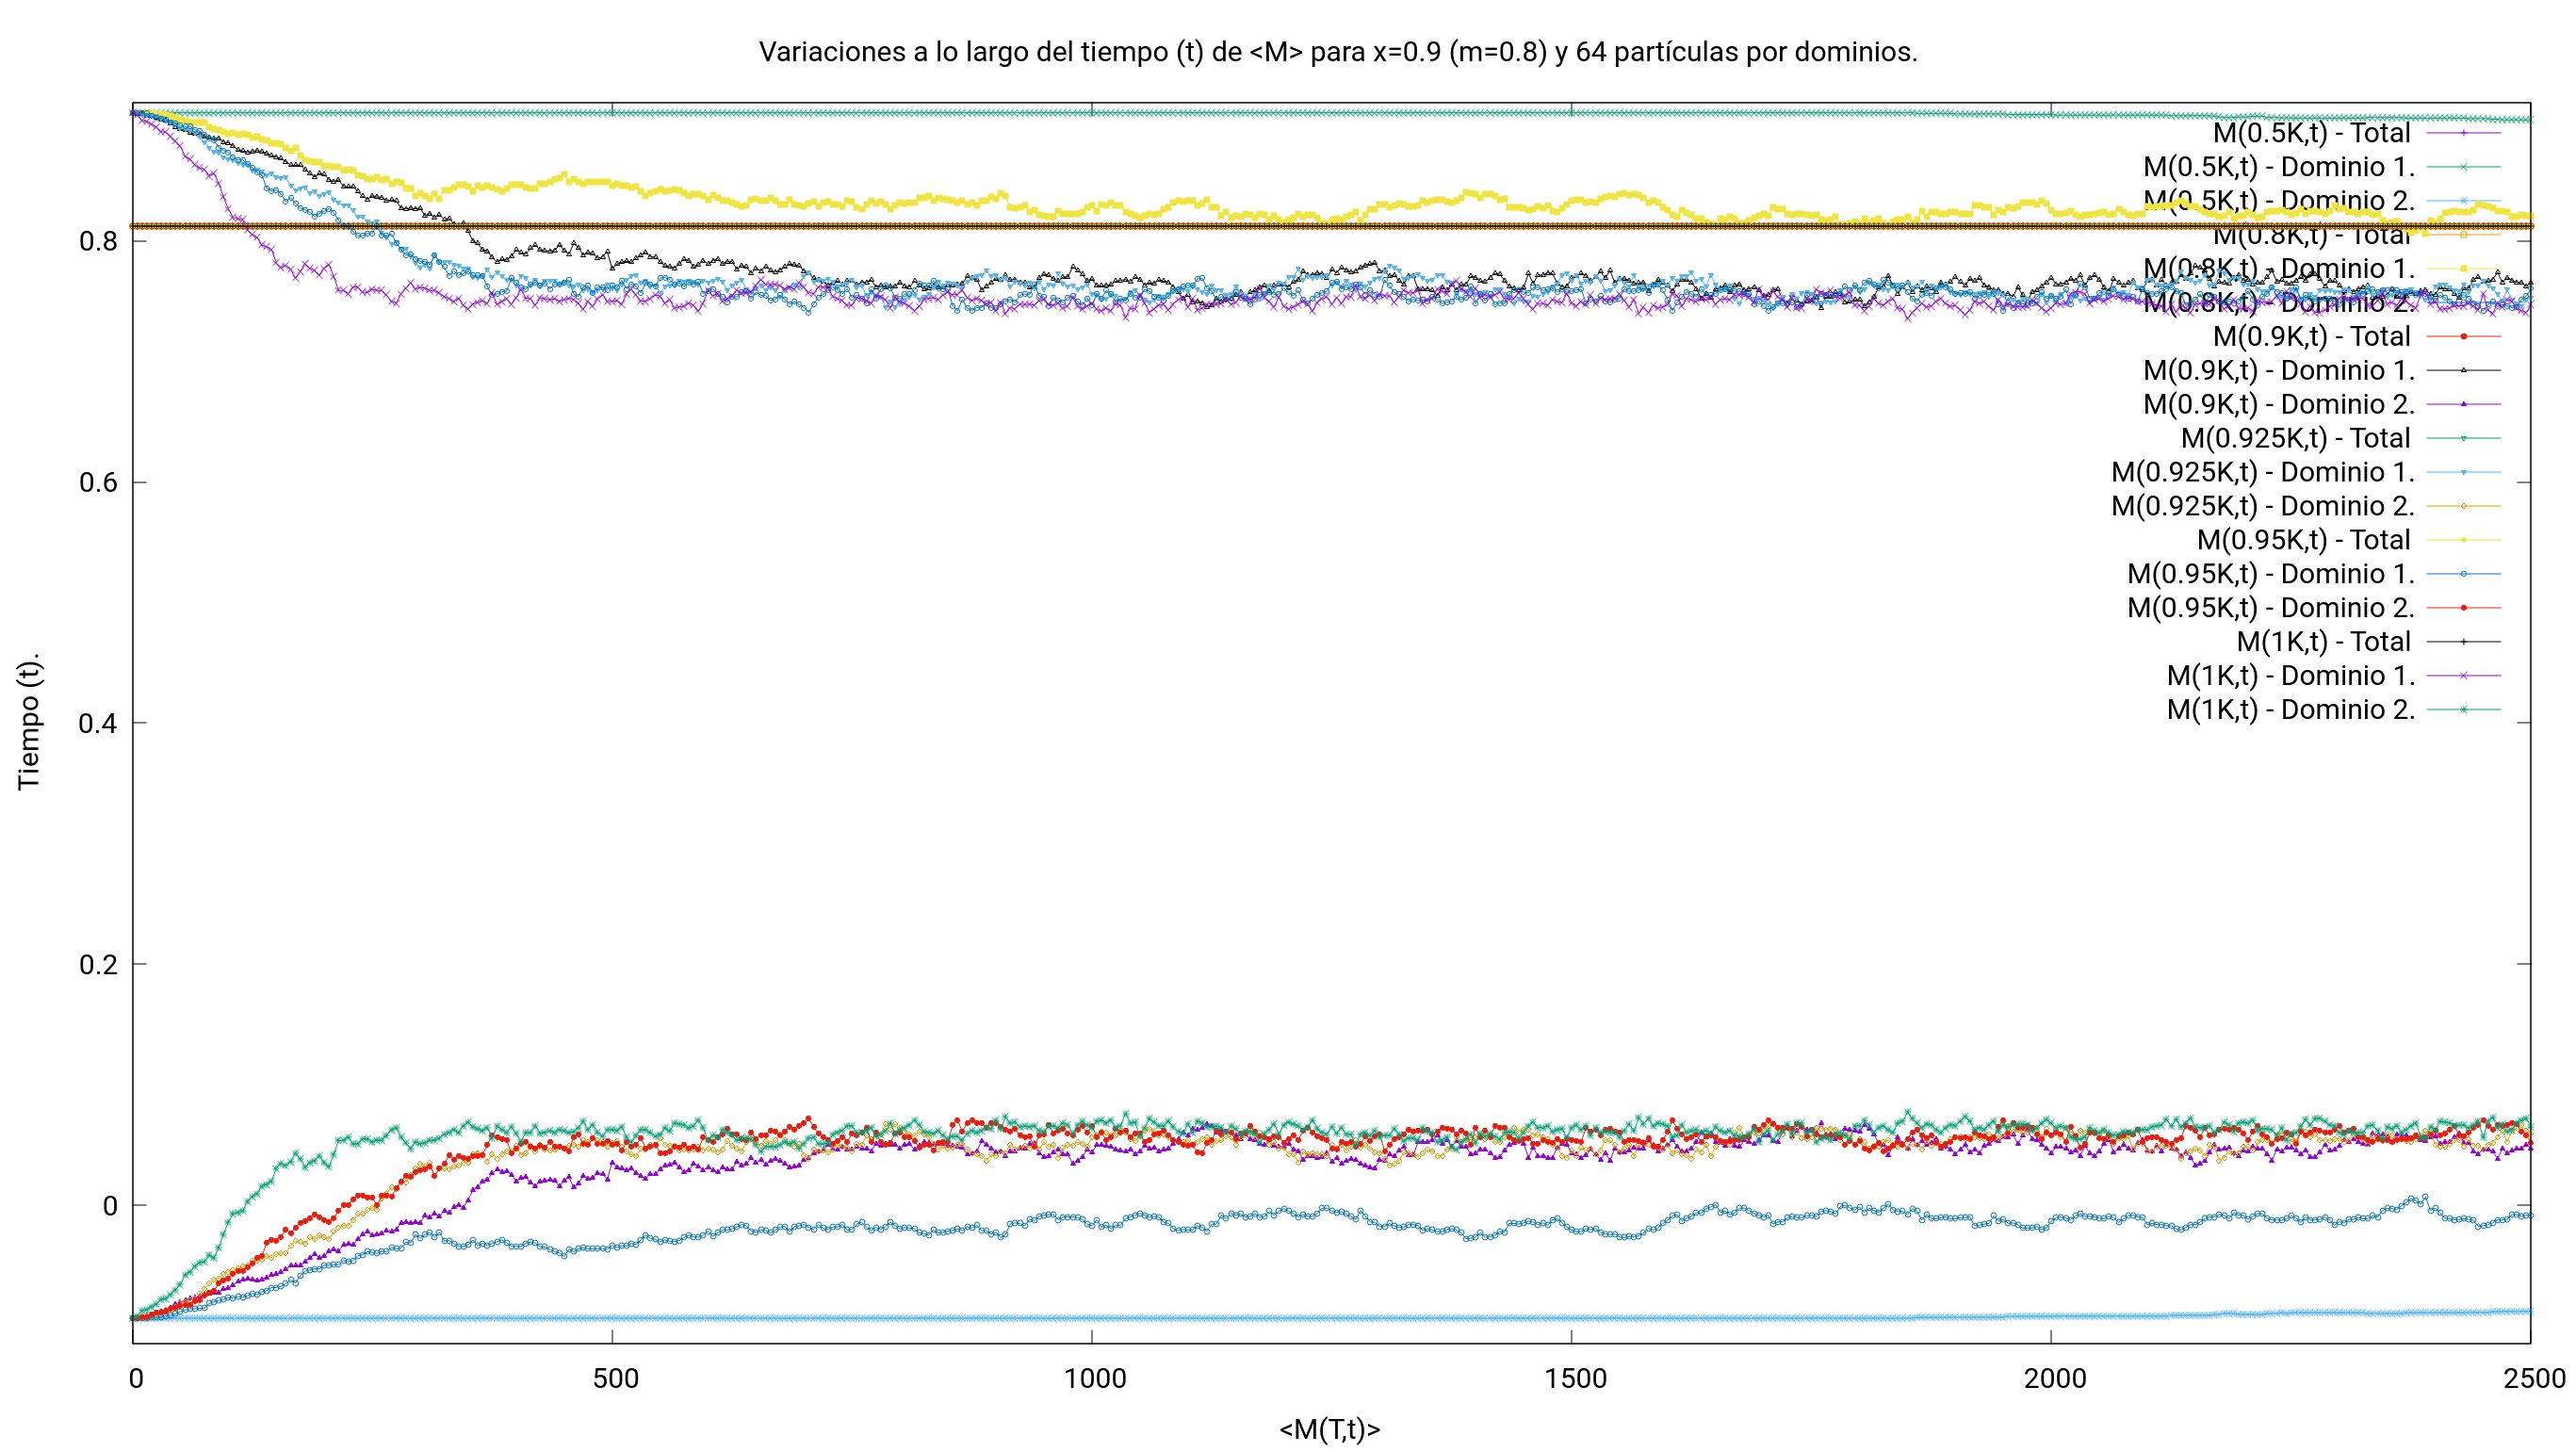
\includegraphics[width=1.1\textwidth]{Imagenes/MagPDom64X90.png}}     
  \end{center}
\end{figure}\\

\begin{figure}[H]
  \begin{center}        
    \caption{Variaciones de la magnetización ($<M(T)>$) por dominios para diferentes temperaturas $(T)$, $X=0.5$ y $128$x$128$ partículas.}
    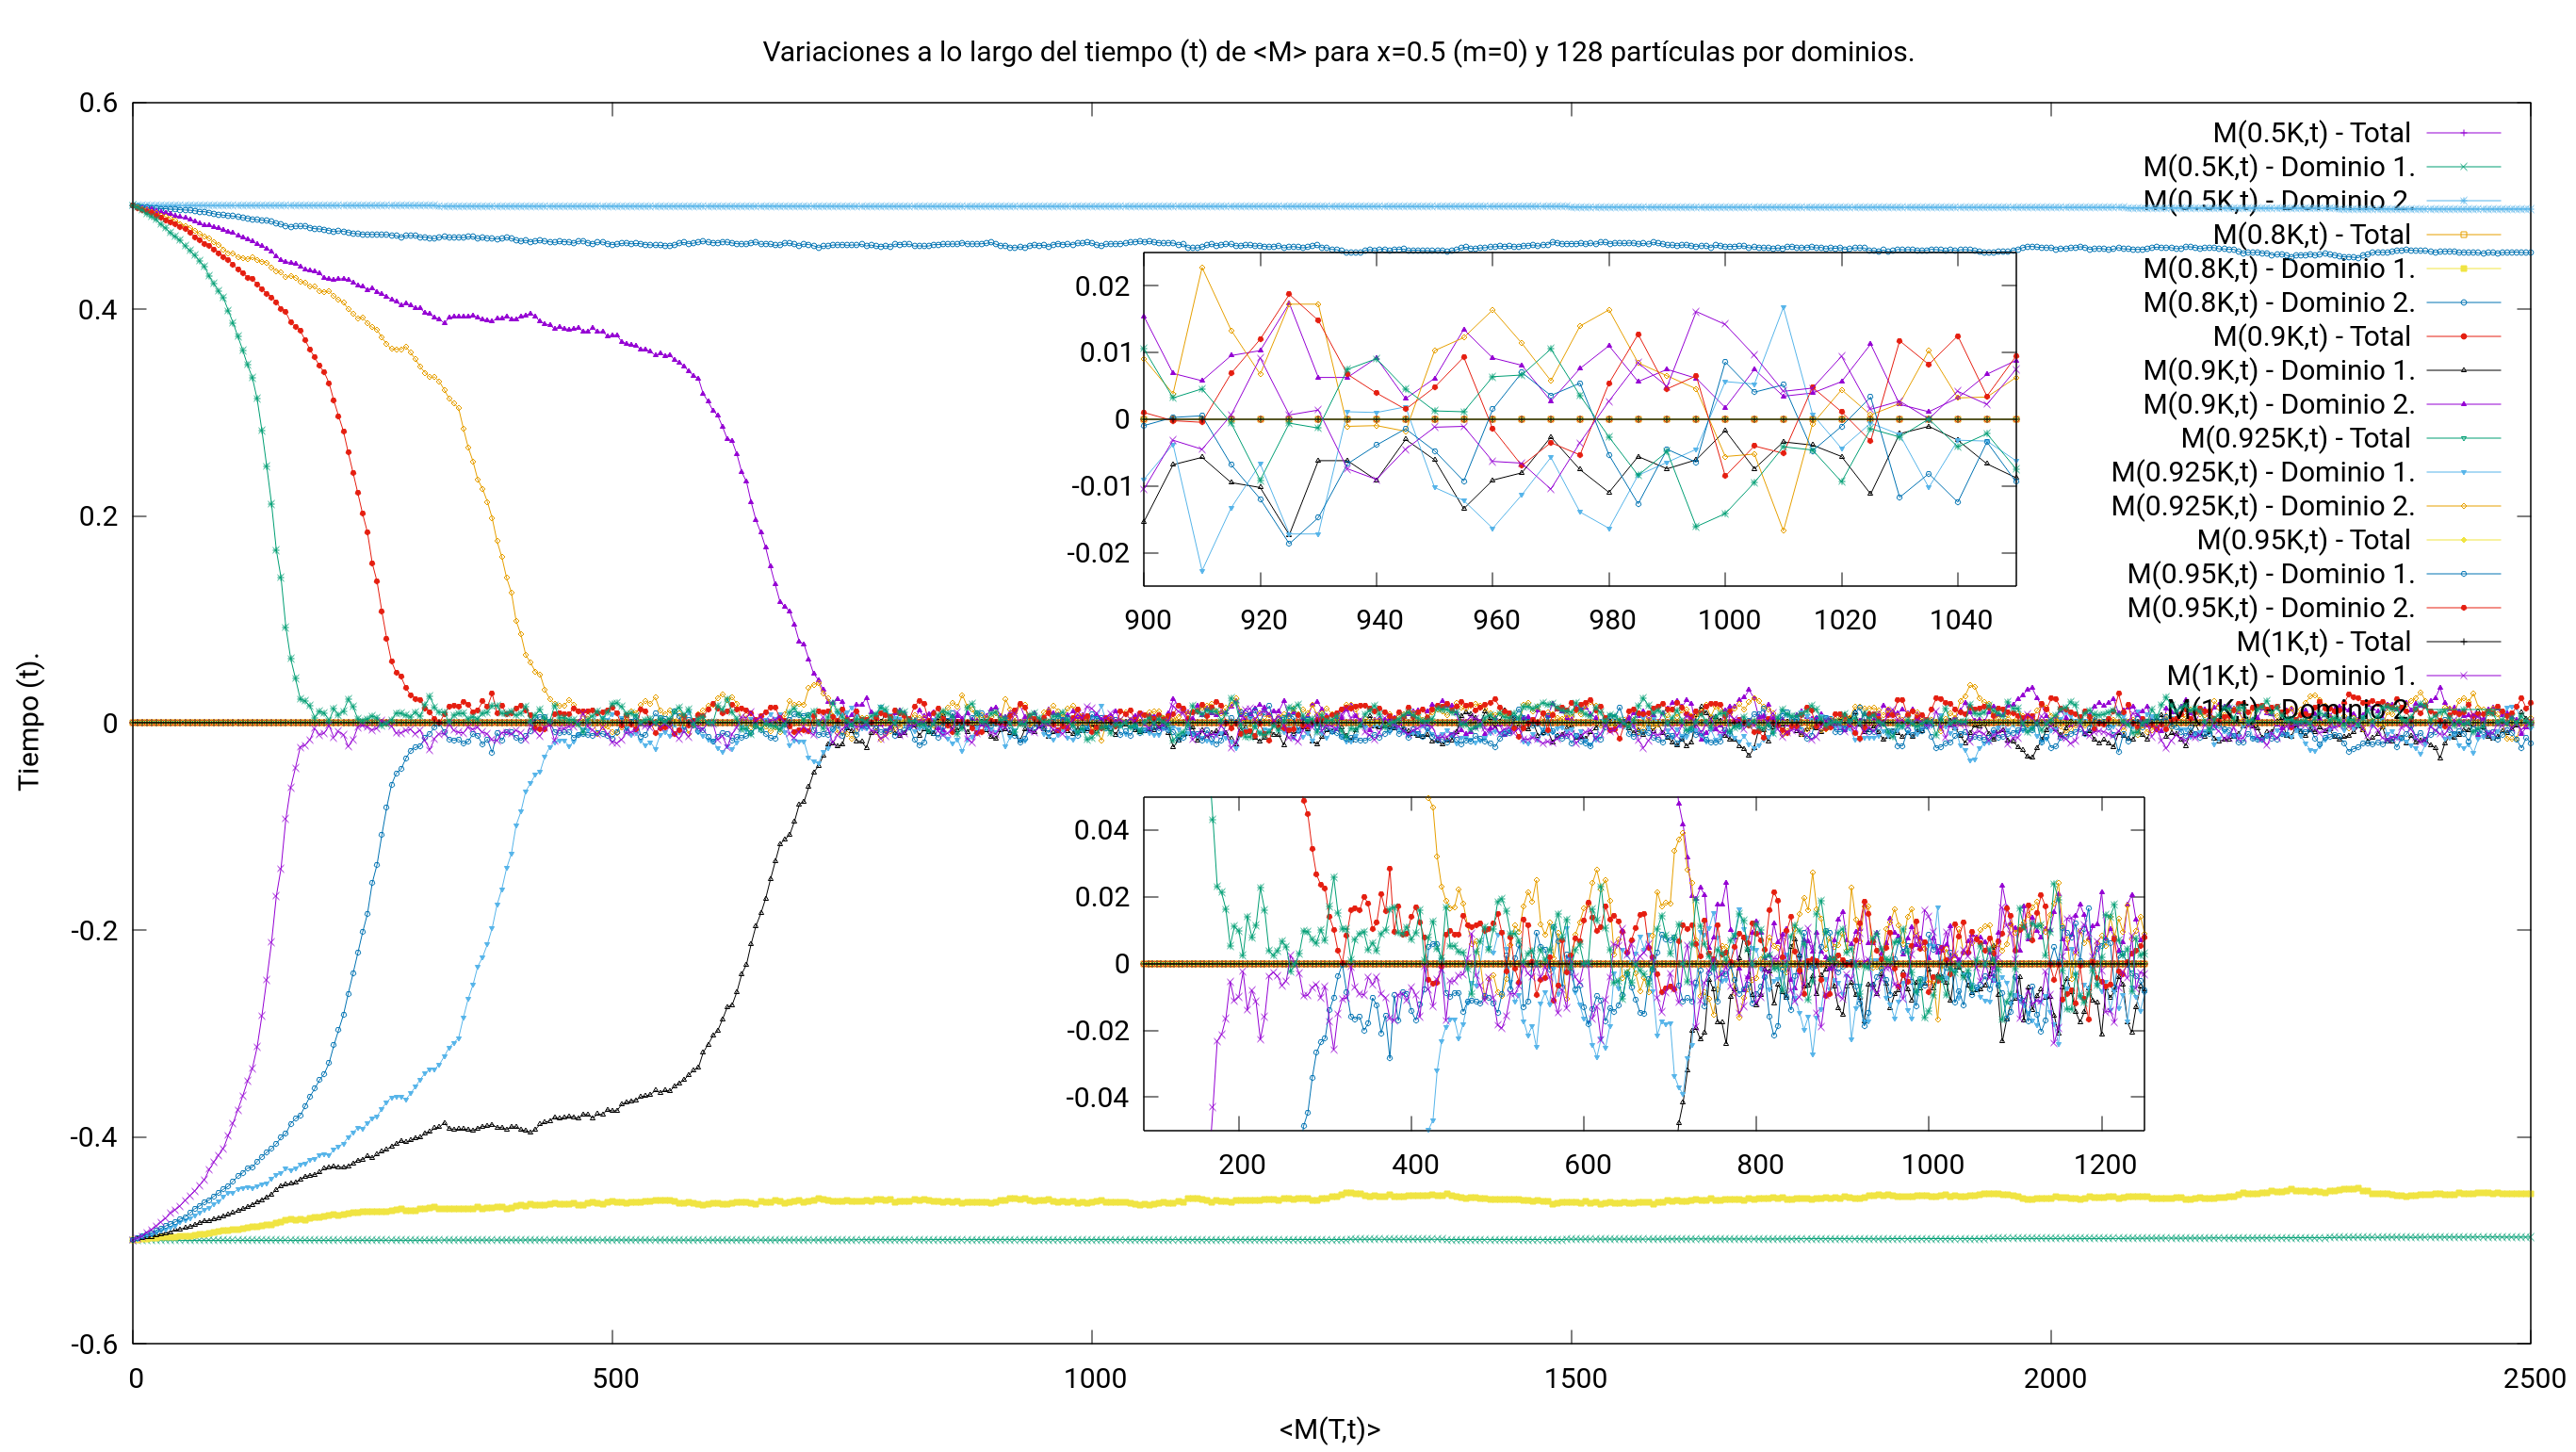
\includegraphics[width=1.1\textwidth]{Imagenes/MagPDom128X50.png}}     
  \end{center}
\end{figure}\\

\begin{figure}[H]
  \begin{center}        
    \caption{Variaciones de la magnetización ($<M(T)>$) por dominios para diferentes temperaturas $(T)$, $X=0.9$ y $128$x$128$ partículas.}
    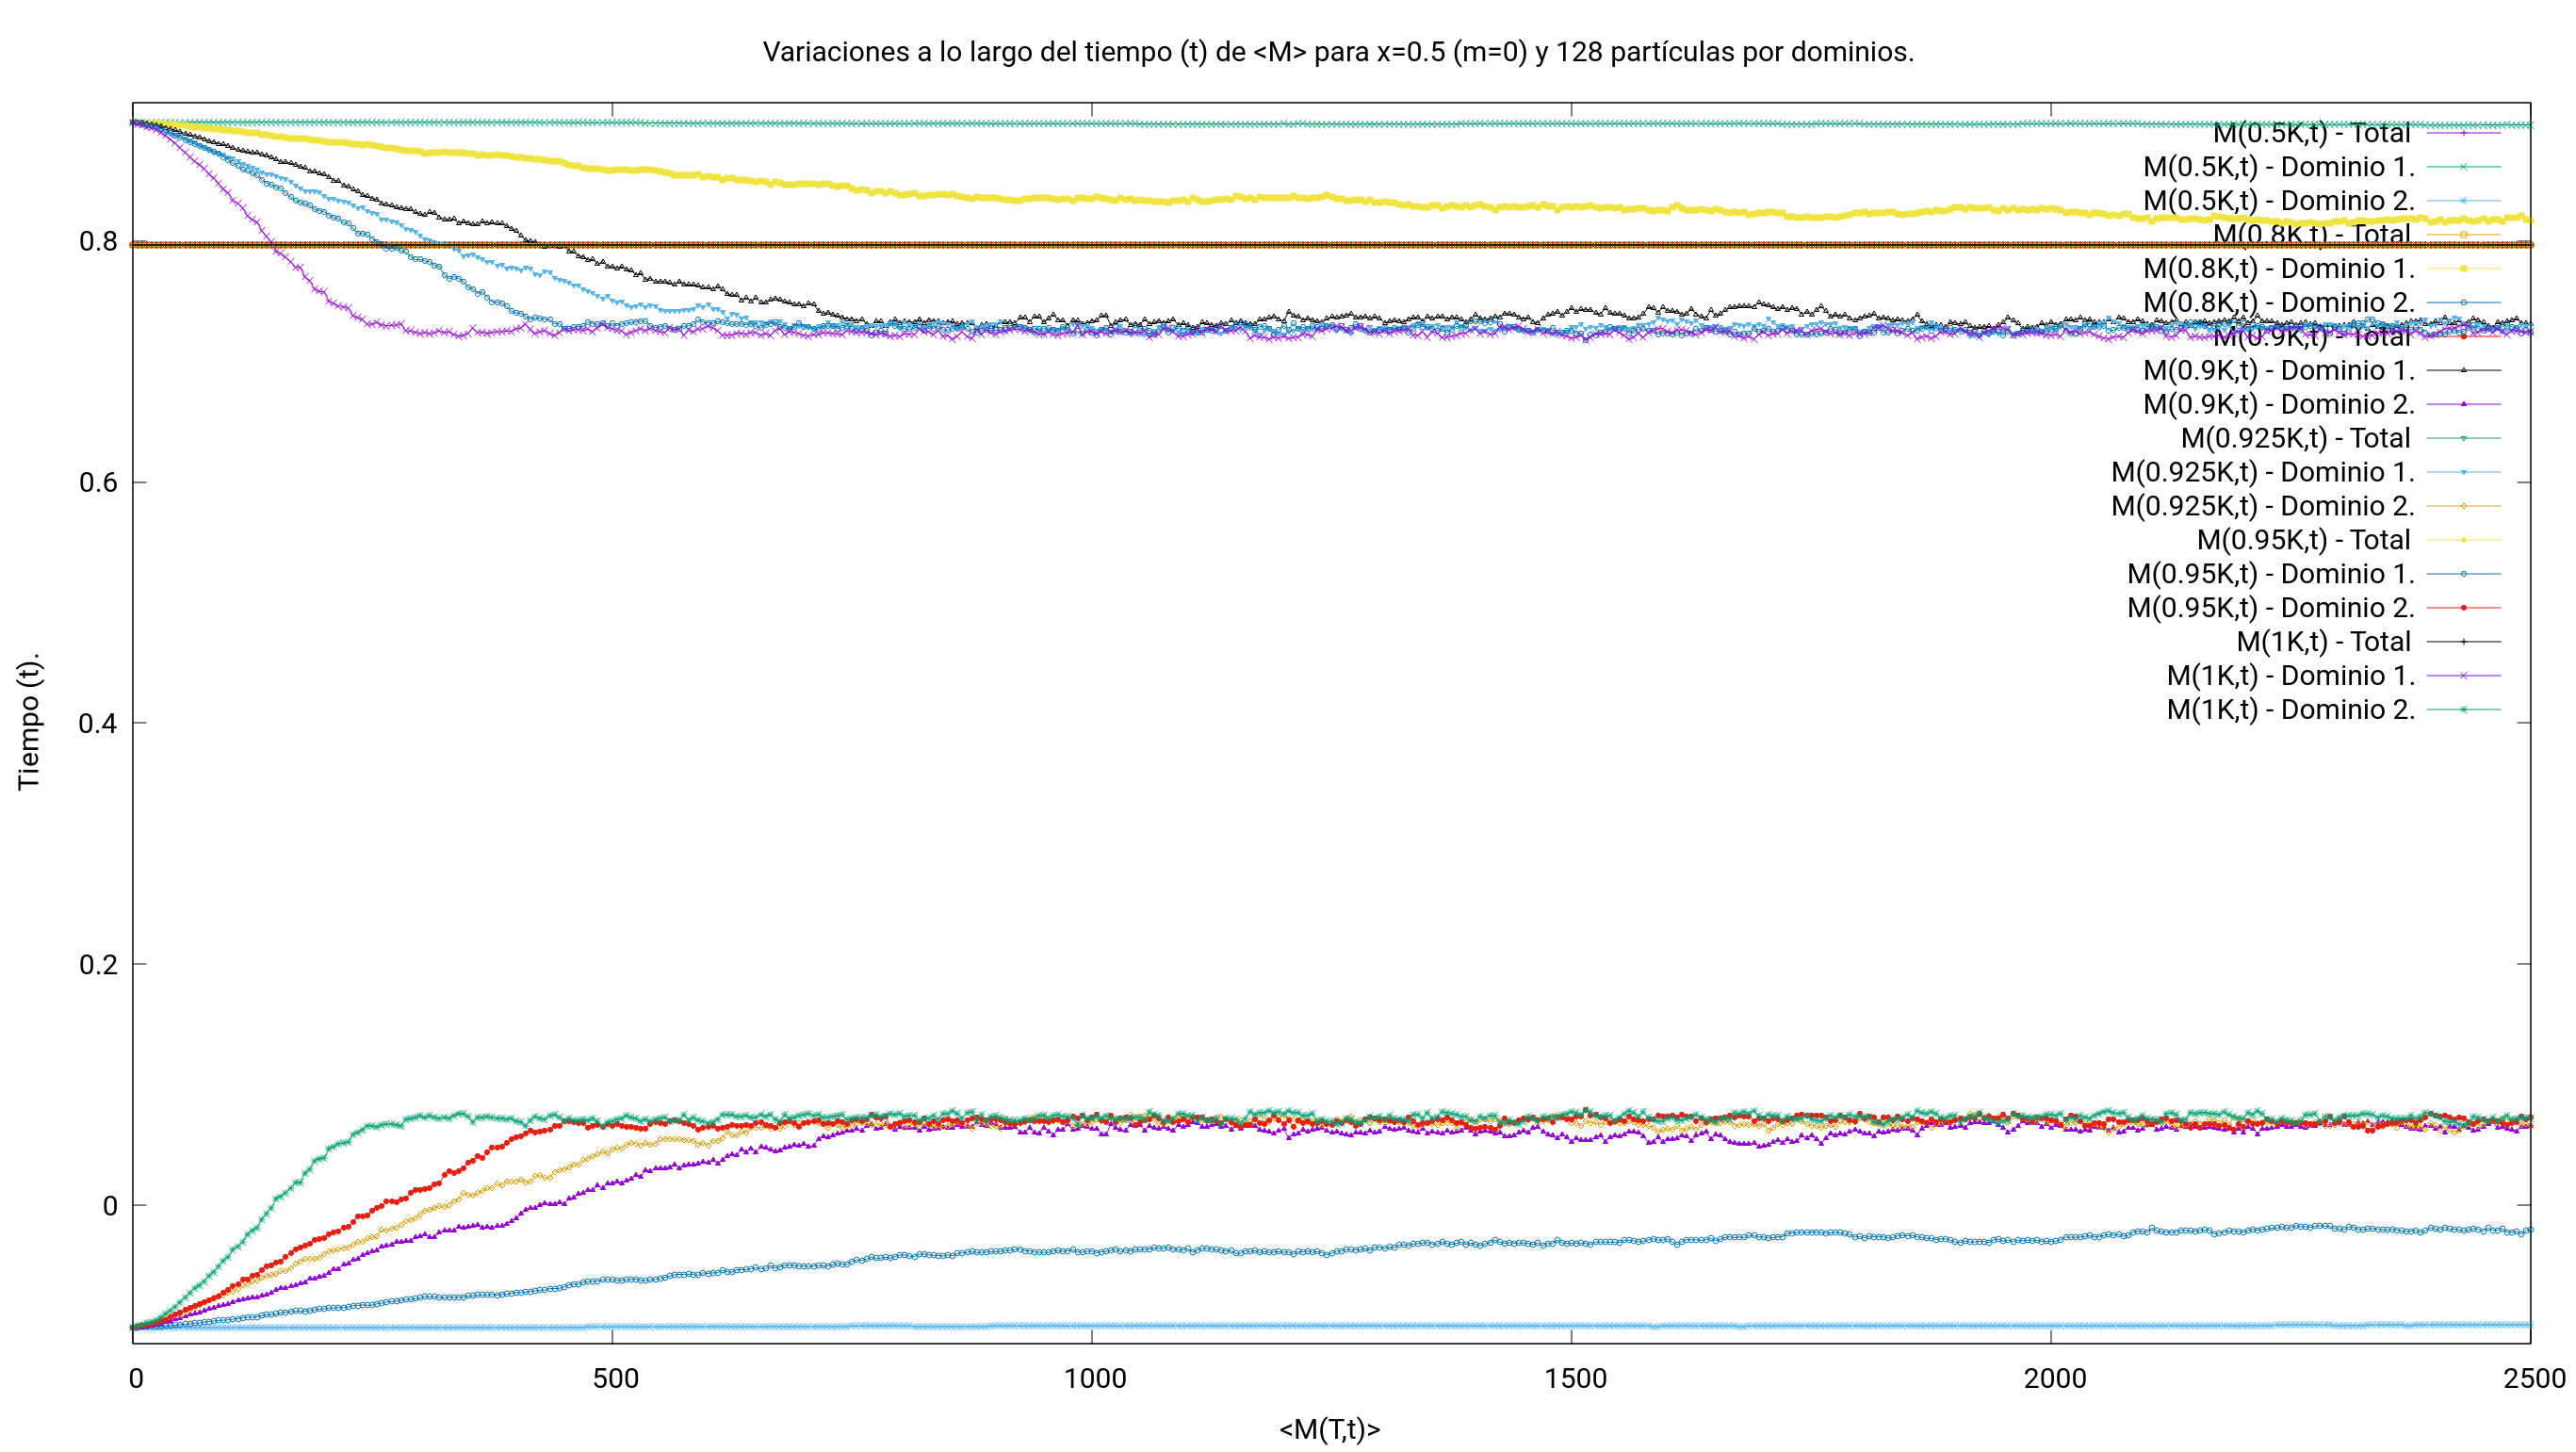
\includegraphics[width=1.1\textwidth]{Imagenes/MagPDom128X90.png}}     
  \end{center}
\end{figure}\\

\begin{figure}[H]
  \begin{center}        
    \caption{Variaciones de la magnetización ($<M(T)>$) por dominios para $T=1k$, $X=0.5$ y diferente número de partículas ($N$).}
    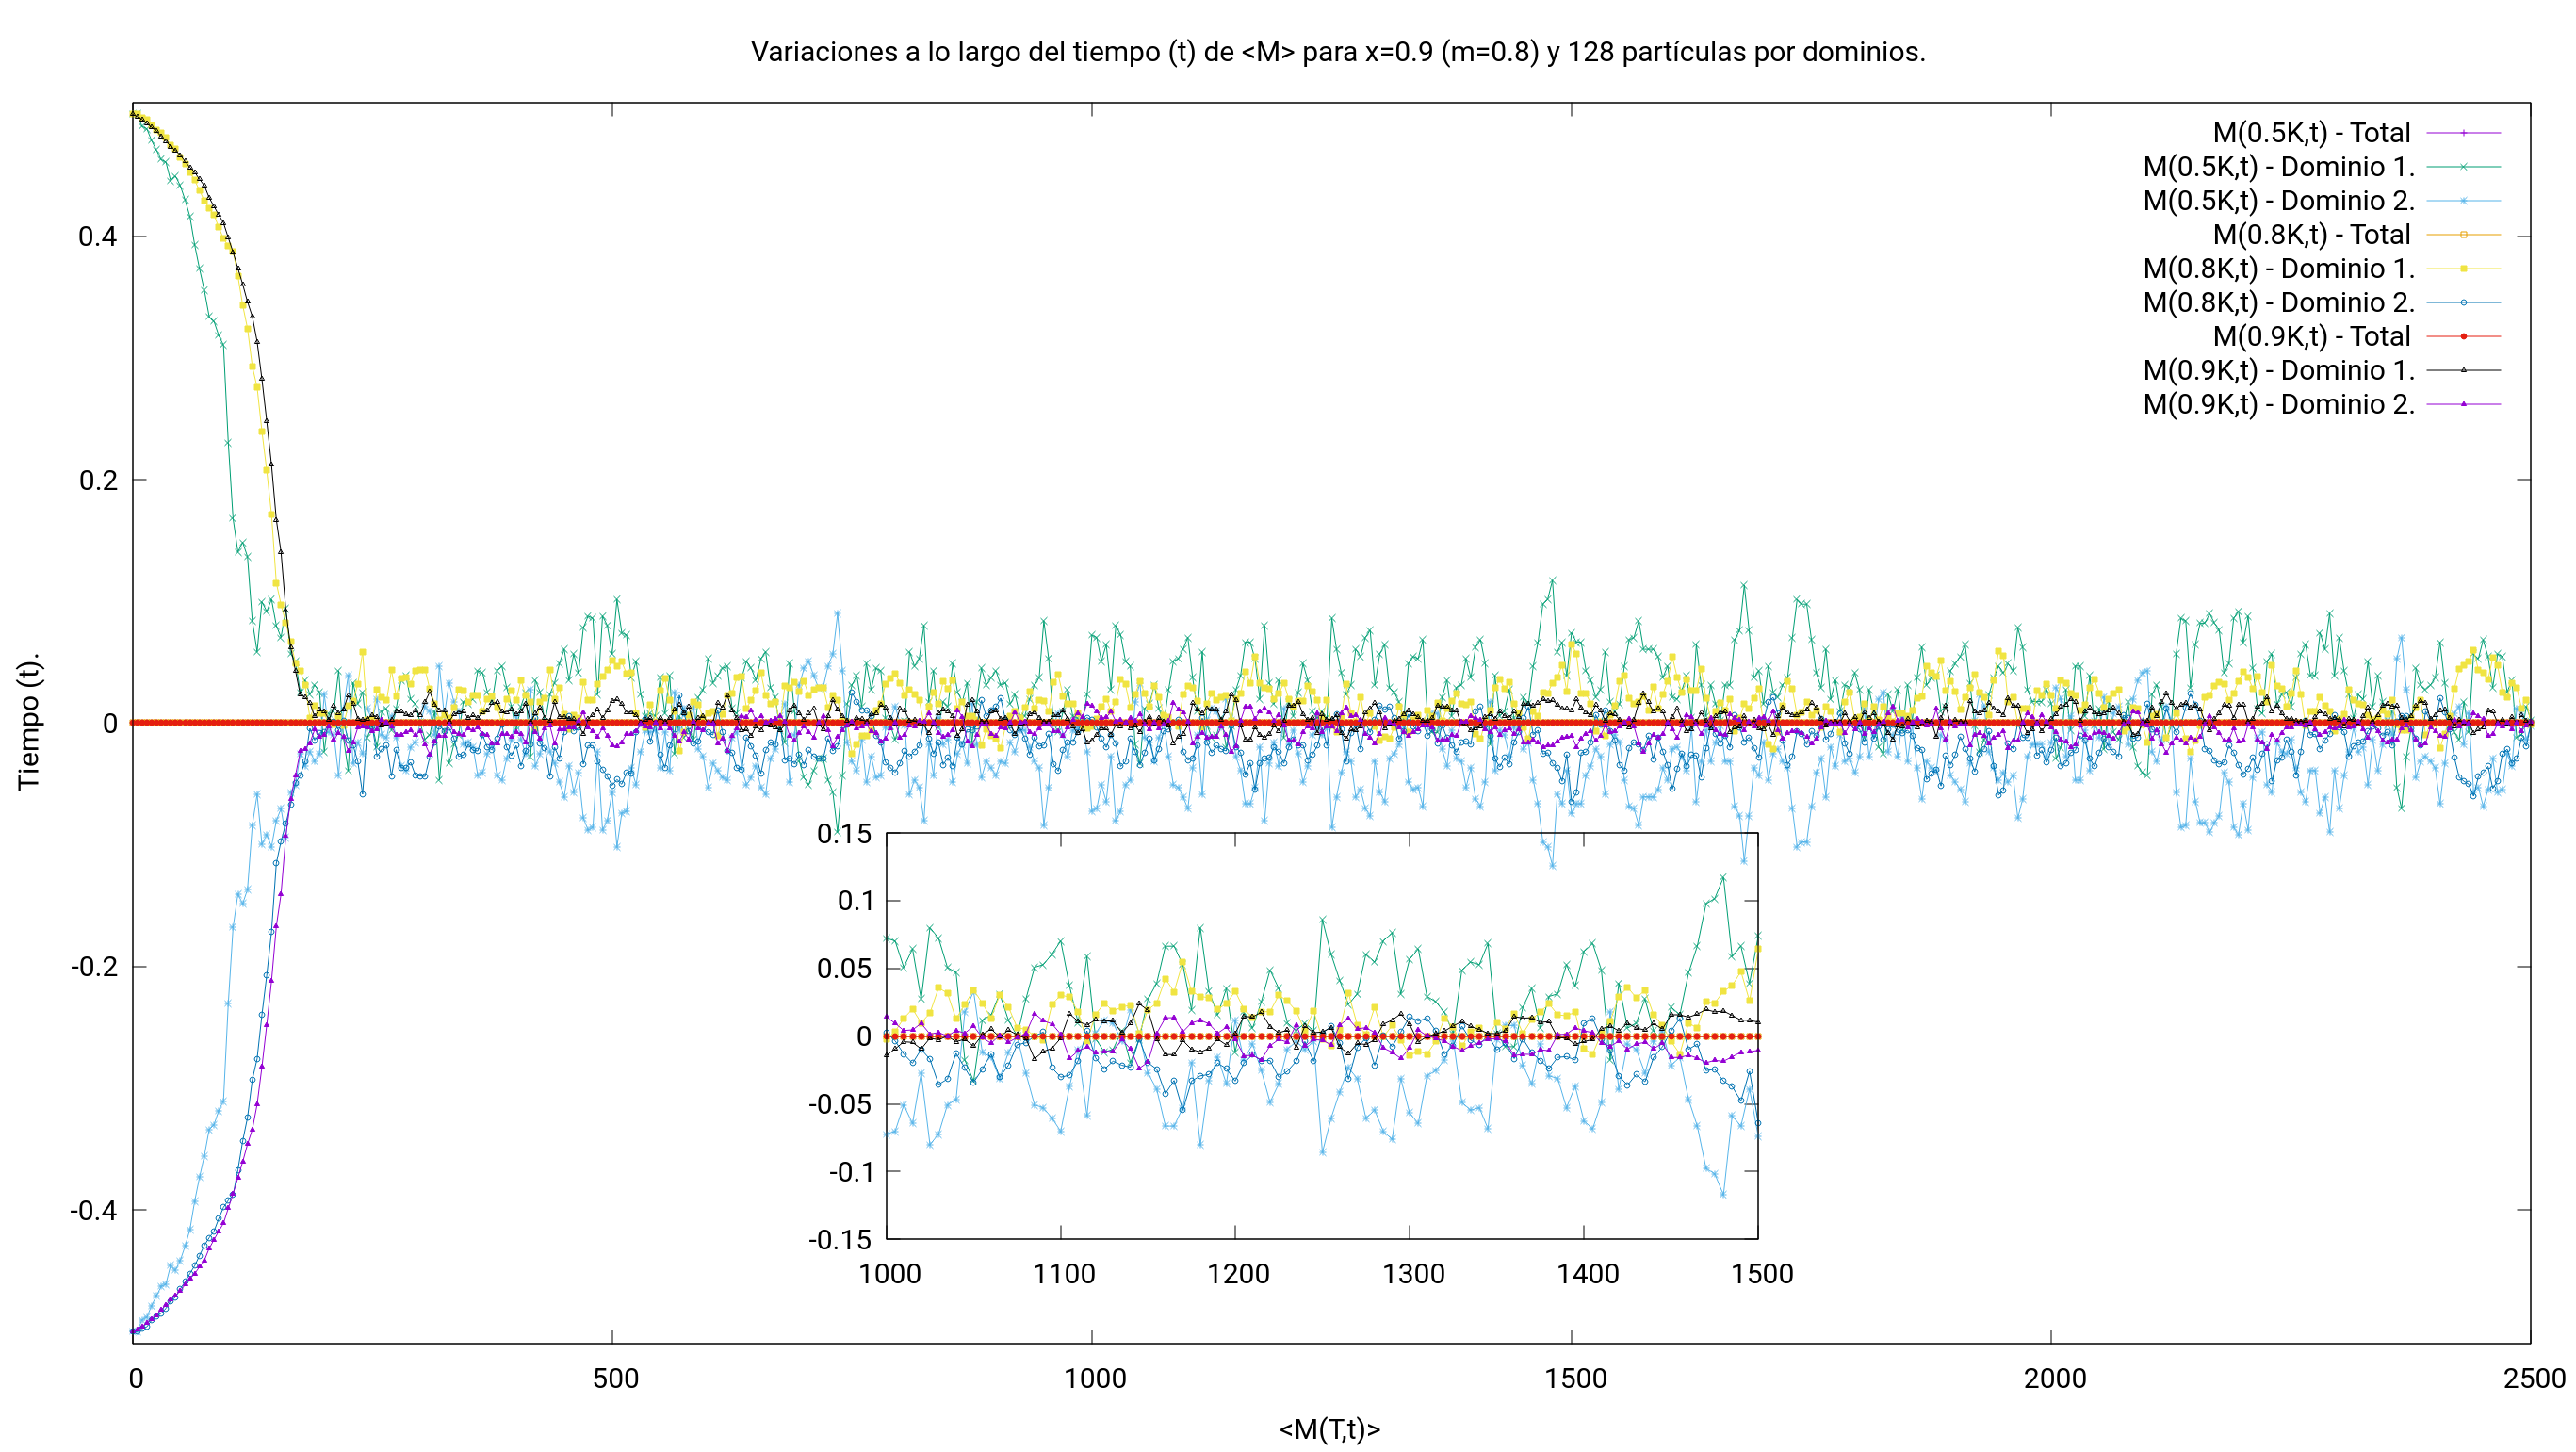
\includegraphics[width=1.1\textwidth]{Imagenes/VarMDomNT1X50.png}}     
  \end{center}
\end{figure}\\

\begin{figure}[H]
  \begin{center}        
    \caption{Variaciones de la magnetización ($<M(T)>$) por dominios para $T=1k$, $X=0.5$ y diferente número de partículas ($N$).}
    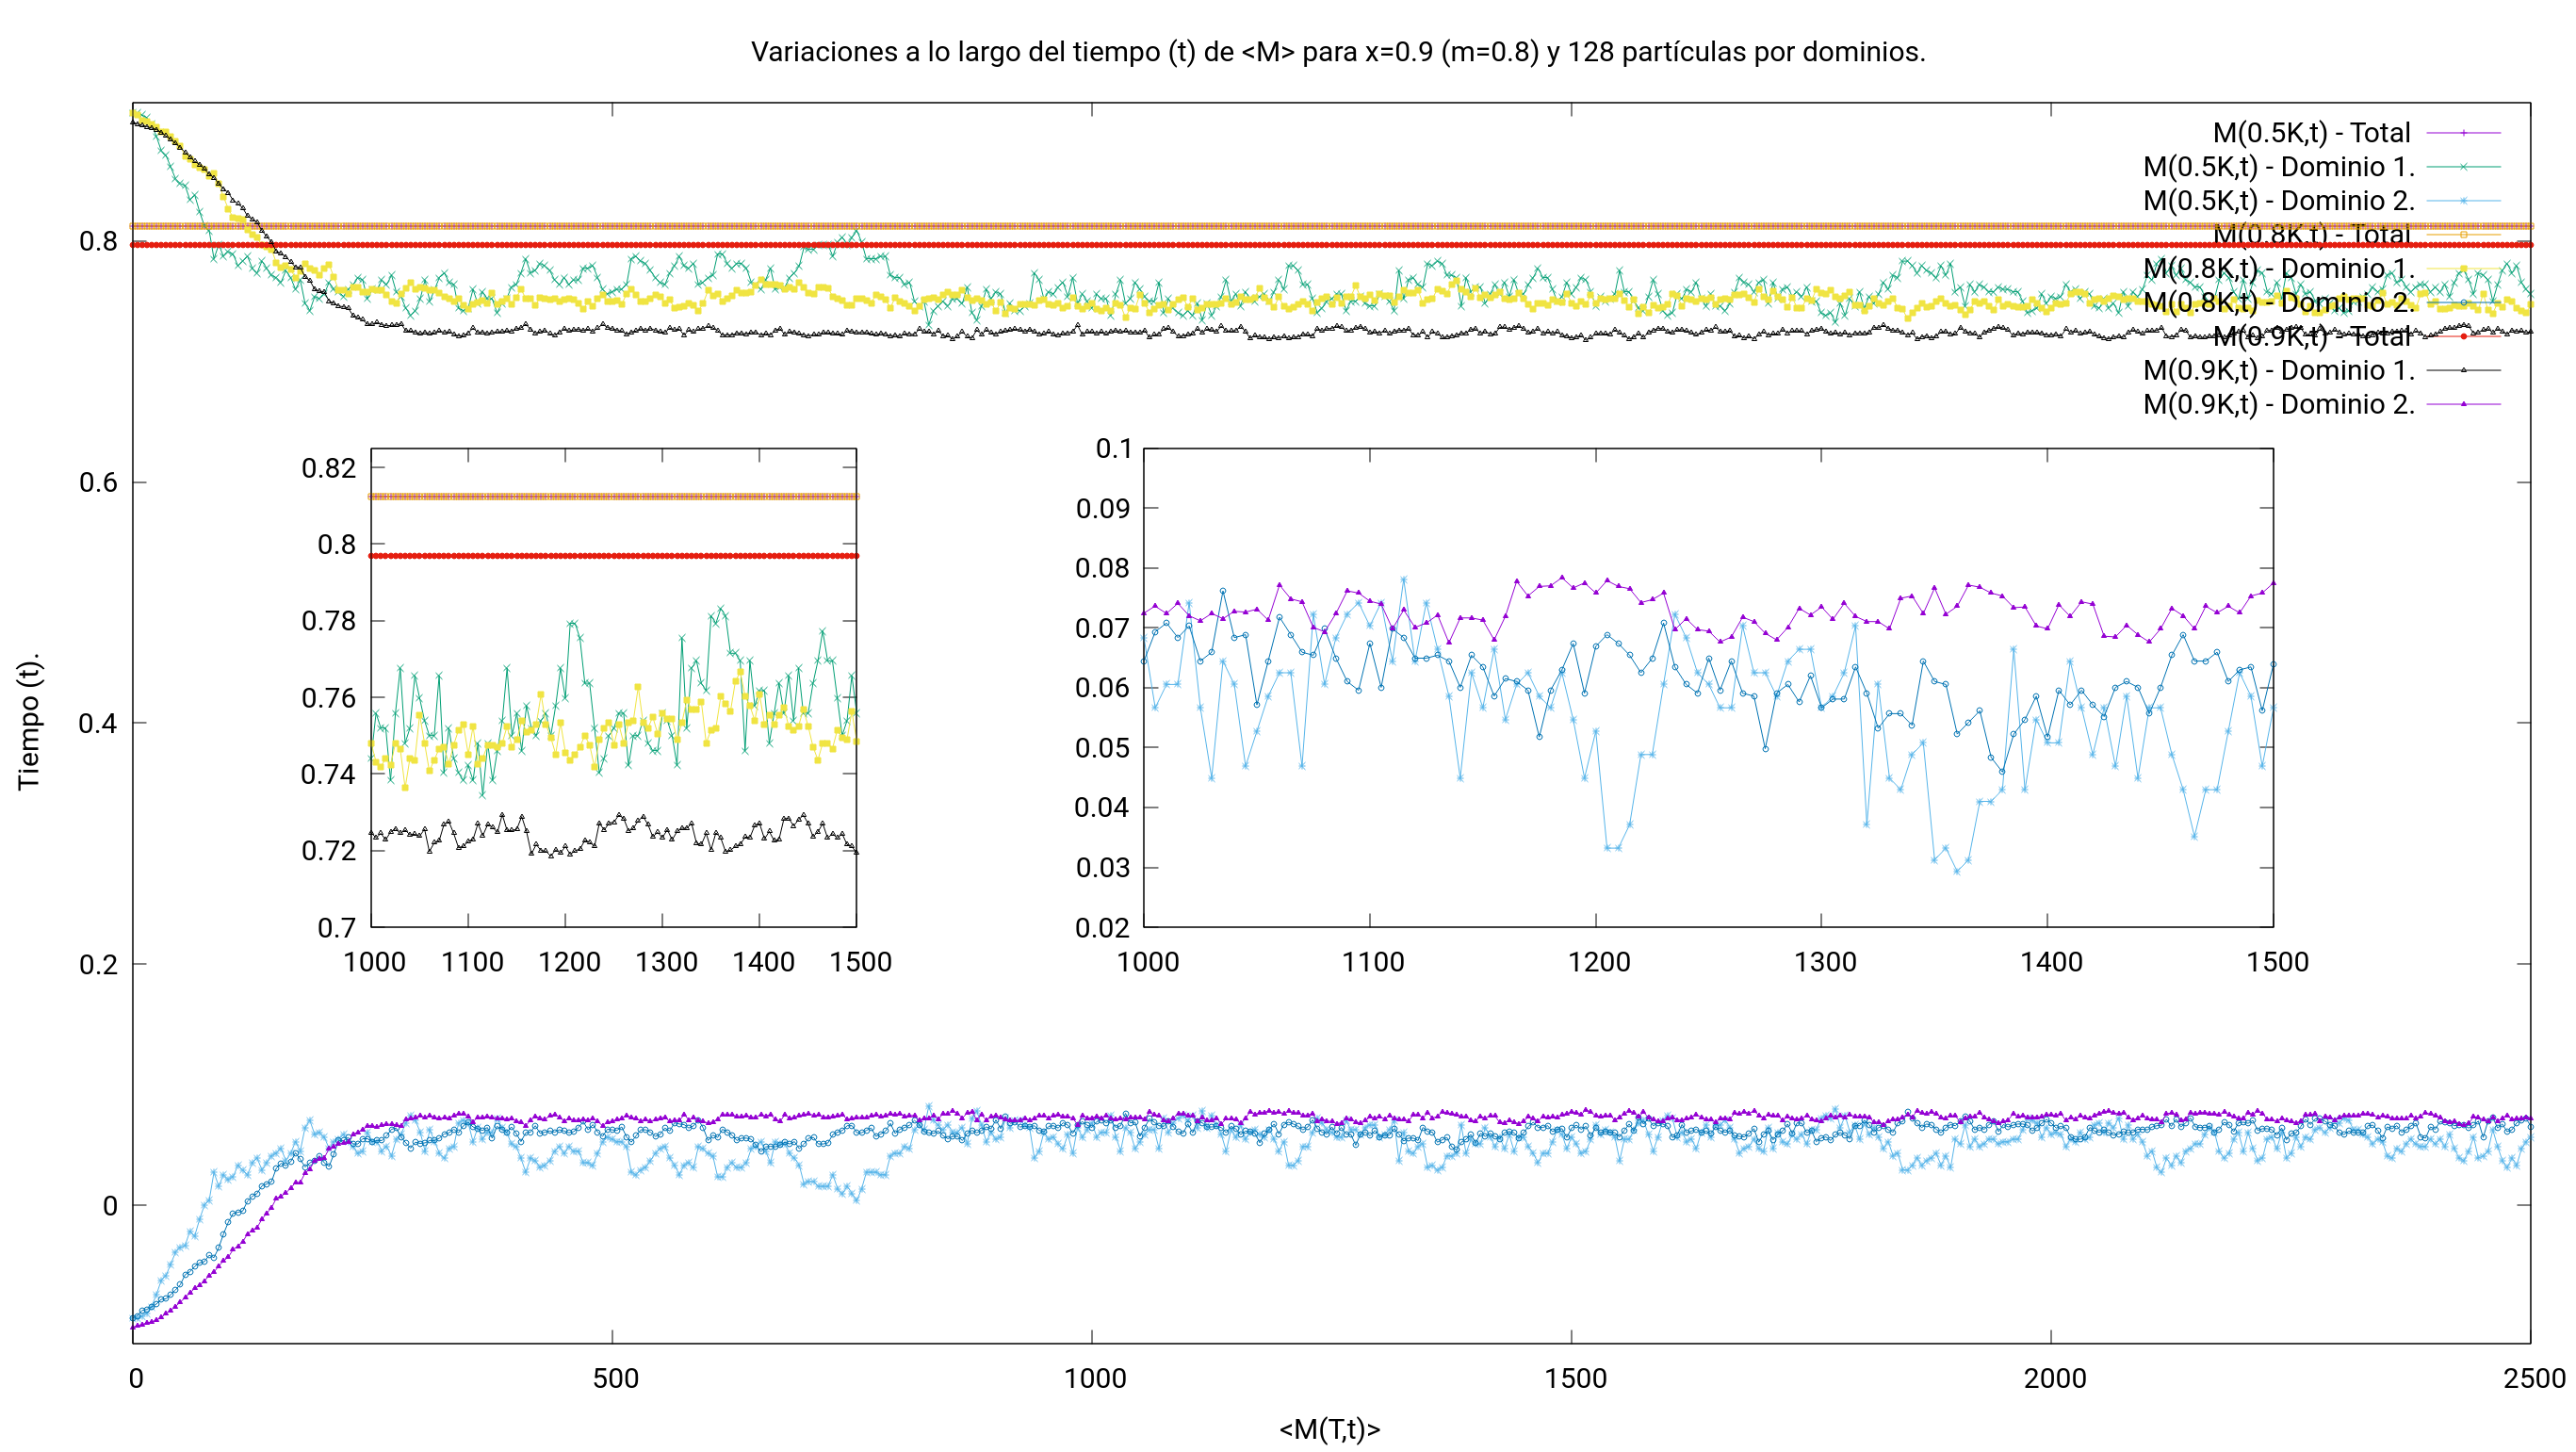
\includegraphics[width=1.1\textwidth]{Imagenes/VarMDomNT1X90.png}}     
  \end{center}
\end{figure}\\

Podemos denotar la clara influencia tanto de $N$ cómo de $T$ siendo cuanto más preciso cuanto mayor es N, y variaciones más bruscas o directas cuanto mayor es N. Por debajo de 0.5K encontramos continuidad absoluta en todos los casos, y a partir de la misma, para temperaturas superiores denotamos claras variaciones y discontinuidades que son debidas claramente al $N$ y $T$ obviamente .\\

Las mismas variaciones, y obviando que se haya cometido algún error tanto de cálculo cómo teórico, pueden ser explicadas tal vez a razones estadísticas (asociadas a la aplicada a este mismo modelo) o que en realidad el sistema físico se comporta de esta manera. En cualquier caso podemos denotar que los resultados tienen sentido los unos con los otros.

\section{Conclusiones.}
Partiendo de la teoría y de unas ecuaciones fundamentales no muy complicadas de entender, podemos modelar de manera muy visual y clara cómo evolucionaría a nivel atómico un material que para bajas temperaturas es ferromagnéticos. El método de Ising nos permite denotar cómo se produce la magnetización espontánea para estos materiales en muchos de sus casos. Pero para el caso en el que queramos que la magnetización inicial se mantenga constante este modelo es el único que nos lo permite. En las figuras \ref{EjemploIsing} y \ref{EjemploIsingKawasaki}, podemos denotar las claras diferencias, y las figuras \ref{fig3} y \ref{fig4} demuestran algunos de los casos que se han estudiado a lo largo de todo el proyecto. Cabe resaltar que se ha realizado todo el trabajo para condiciones de contorno periódicas en el eje x y fijas en el eje y. salvo para las primeras gráficas donde son periódicas en ambos ejes.\\

Por otro lado cabe resaltar el estudio que se ha realizado sobre el calor específico ($C_N$) y la susceptibilidad magnética ($\chi_N$) que se ha realizado. Destacar las figuras \ref{xn05}, \ref{cn05}, \ref{cn09} y \ref{xn09}, que nos han permitido comprobar con considerable claridad el ferromagnetismo así cómo se ajustan los modelos teóricos a los numéricos de una manera casi precisa y perfecta. Aun más importante, hemos podido comprobar la validez del calculo numérico realizado así cómo del modelo llevado a cabo con los ajuste a los valores teóricos que debería de tener la susceptibilidad magnética ($\chi_N$), así cómo de la obtención de $T_C$ (en nuestro caso $T_C \approx 0.9$) comprobando los resultados experimentales (figura \ref{fig9}) con los teóricos mostrados en el capítulo 5 del libro de Newman.\\

Finalmente, hemos podido denotar las variaciones que tanto de la energía media ($<E>$) del sistema cómo de la magnetización ($<M>$) para varios casos considerablemente diferentes, para particiones del sistema del $50 \%$ y $90 \%$, siendo sus magnetizaciones constantes del valor $m=0$ y $m=0.8$ respectivamente, para diferentes temperaturas centradas entorno a $T_C$, y para $N= 32^2, \hspace{1mm} 64^2 \hspace{1mm} y \hspace{1mm} 128^2$ partículas. Denotando una clara continuidad de la magnetización para valores por debajo de 0.5, considerables rápidas variaciones cuanto mayor es la temperatura, la conservación de la magnetización y sus correspondientes variaciones por dominios o por cortes en el eje y, y la maximización de la energía para temperaturas cercanas al 0 absoluto.



\newpage
\begin{thebibliography}{}

\bibitem{}
ising-SLIDESv2.pdf. Física Computacional. Grado en Física. Prado.

\bibitem{}
problema$\_$Ising-Kawasaki.pdf. Física Computacional. Grado en Física. Prado.

\bibitem{}
chapter$\_$5$\_$Newman$\_$Barkema.pdf. Física Computacional. Grado en Física. Prado.

\bibitem{}
https://es.wikipedia.org/wiki/Modelo$\_$de$\_$Ising

\bibitem{}
https://valbuena.fis.ucm.es/expint/html/fises/ising/ising.html

\end{thebibliography}

\end{document}